% !Mode:: "TeX:UTF-8"
%%%%%%%%%%%%%%%%%%%%%%%%%%%%%%%%%%%%%%%%%%%%%%%%%%%%%%%%%%%%%%%%%%%%%%%%%%%%%%%%
%          ,
%      /\^/`\
%     | \/   |                CONGRATULATIONS!
%     | |    |             SPRING IS IN THE AIR!
%     \ \    /                                                _ _
%      '\\//'                                               _{ ' }_
%        ||                     hithesis v3                { `.!.` }
%        ||                                                ',_/Y\_,'
%        ||  ,                   dustincys                   {_,_}
%    |\  ||  |\          Email: yanshuoc@gmail.com             |
%    | | ||  | |            https://yanshuo.name             (\|  /)
%    | | || / /                                               \| //
%    \ \||/ /       https://github.com/dustincys/hithesis      |//
%      `\\//`   \\   \./    \\ /     //    \\./   \\   //   \\ |/ /
%     ^^^^^^^^^^^^^^^^^^^^^^^^^^^^^^^^^^^^^^^^^^^^^^^^^^^^^^^^^^^^^^
%%%%%%%%%%%%%%%%%%%%%%%%%%%%%%%%%%%%%%%%%%%%%%%%%%%%%%%%%%%%%%%%%%%%%%%%%%%%%%%%
\documentclass[fontset=fandol,type=doctor,campus=harbin]{hithesisbook}
% 此处选项中不要有空格
%%%%%%%%%%%%%%%%%%%%%%%%%%%%%%%%%%%%%%%%%%%%%%%%%%%%%%%%%%%%%%%%%%%%%%%%%%%%%%%%
% 必填选项
% type=doctor|master|bachelor|postdoc
%%%%%%%%%%%%%%%%%%%%%%%%%%%%%%%%%%%%%%%%%%%%%%%%%%%%%%%%%%%%%%%%%%%%%%%%%%%%%%%%
% 选填选项(选填选项的缺省值已经尽可能满足了大多数需求,除非明确知道自己有什么
% 需求)
% campus=shenzhen|weihai|harbin
%   含义:校区选项,默认harbin
% glue=true|false
%   含义:由于我工规范中要求字体行距在一个闭区间内,这个选项为true表示tex自
%   动选择,为false表示区间内一个最接近版心要求行数的要求的默认值,缺省值为
%   false。
% tocfour=true|false
%   含义:是否添加第四级目录,只对本科文科个别要求四级目录有效,缺省值为
%   false
% fontset=windows|mac|ubuntu|fandol|adobe
%   含义:设置字体,默认情况会自动识别系统,然后设置字体。后两个是开源字体,自行
%   下载安装后设置使用。windows是中易字库,窝工默认常用字体,绝对没毛病。mac和
%   ubuntu 默认分别是华文和思源字库,理论上用什么字库都行。后两种开源字库的安装
%   方法到谷歌上百度一下什么都有了。Linux非ubuntu发行版、非x86架构机器等如何运行
%   可到github issue上讨论。
% tocblank=true|false
%   含义:目录中第一章之前,是否加一行空白。缺省值为true。
% chapterhang=true|false
%   含义:目录的章标题是否悬挂居中,规范中要求章标题少于15字,所以这个选项
%   有无没什么用,除了特殊需求。缺省值为true。
% fulltime=true|false
%   含义:是否全日制,缺省值为true。非全日制如同等学力等,要在cover中设置类
%   型,封面中不同格式
% subtitle=true|false
%   含义:论文题目是否含有副标题,缺省值为false,如果有要在cover中设置副标
%   题内容,封面中显示。
% newgeometry=one|two|no
%   含义:规范中的自相矛盾之处,版芯是否包含页眉页脚,旧方法是按照包含页眉
%   页脚来设置。该选项是多选选项,如果设置为no,则版新为旧模板的版芯设置方法,
%   如果设置该选项one或two,分别对应两种页眉页码对应版芯线的相对位置。第一种
%   是严格按照规范要求,难看。第二种微调了页眉页码位置,好一点。默认two。
% debug=true|false
%   含义:是否显示版芯框和行号,用来调试。默认否。
% openright=true|false
%   含义:博士论文是否要求章节首页必须在奇数页,此选项不在规范要求中,按个
%   人喜好自行决定。 默认否。注意,窝工的默认情况是打印版博士论文要求右翻页
%   ,电子版要求非右翻页且无空白页。如果想DIY(或身不由己DIY)在什么地方右
%   翻页,将这个选项设置为false,然后在目标位置添加`\cleardoublepage`命令即
%   可。
% library=true|false
%   含义:是否为提交到图书馆的电子版。默认否。注意:如果设置成true,那么
%   openright选项将被强制转换为false。
% capcenterlast=true|false
%   含义:图题、表题最后一行是否居中对齐(我工规范要求居中,但不要求居中对
%   齐),此选项不在规范要求中,按个人喜好自行决定。默认否。
% subcapcenterlast=true|false
%   含义:子图图题最后一行是否居中对齐(我工规范要求居中,但不要求居中对齐
%   ),此选项不在规范要求中,按个人喜好自行决定。默认否。
% absupper=true|false
%   含义:中文目录中的英文摘要在中文目录中的大小写样式歧义,在规范中要求首
%   字母大写,在work样例中是全大写。该选项控制是否全大写。默认否。
% bsmainpagenumberline=true|false
%   含义:由于本科生论文官方模板的页码和页眉格式混乱,提供这个选项自定义设
%   置是否在正文中显示页码横线,默认否。
% bsfrontpagenumberline=true|false
%   含义:由于本科生论文官方模板的页码和页眉格式混乱,提供这个选项自定义设
%   置是否在前文中显示页码横线,默认否。
% bsheadrule=true|false
%   含义:由于本科生论文官方模板的页码和页眉格式混乱,提供这个选项自定义设
%   置是否显示页眉横线,默认显示。
% splitbibitem=true|false
%   含义:参考文献每一个条目内能不能断页,应广大刀客要求添加。默认否。
% newtxmath=true|false
%   含义:数学字体是否使用新罗马。默认是。
% chapterbold=true|false
%   含义:本科生章标题在目录和正文中是否加粗
% engtoc=true|false
%   含义:非博士生需要添加英文目录的,手动添加,如果是博士,此开关无效
% zijv=word|regu
%   含义:字距设置为规范规定33个字还是word中34个字。默认regu。
%%%%%%%%%%%%%%%%%%%%%%%%%%%%%%%%%%%%%%%%%%%%%%%%%%%%%%%%%%%%%%%%%%%%%%%%%%%%%%%%
\usepackage{hithesis}

\graphicspath{{figures/}}

\begin{document}
\frontmatter
% !Mode:: "TeX:UTF-8"

\hitsetup{
  %******************************
  % 注意:
  %   1. 配置里面不要出现空行
  %   2. 不需要的配置信息可以删除
  %******************************
  %
  %=====
  % 秘级
  %=====
  statesecrets={公开},
  natclassifiedindex={TM301.2},
  intclassifiedindex={62-5},
  %
  %=========
  % 中文信息
  %=========
  %ctitleone={局部多孔质气体静压},%本科生封面使用
  %ctitletwo={轴承关键技术的研究},%本科生封面使用
  ctitlecover={基于深度学习的中文语义依存图\\分析技术研究},%放在封面中使用,自由断行
  ctitle={局部多孔质气体静压轴承关键技术的研究},%放在原创性声明中使用
  %csubtitle={一条副标题}, %一般情况没有,可以注释掉
  cxueke={工学},
  csubject={计算机科学与技术},
  caffil={计算机科学与技术学院},
  cauthor={王宇轩},
  csupervisor={车万翔教授},
  %cassosupervisor={某某某教授}, % 副指导老师
  %ccosupervisor={某某某教授}, % 联合指导老师
  % 日期自动使用当前时间,若需指定按如下方式修改:
  cdate={2021年8月},
  cstudentid={16B903007},
  cstudenttype={学术学位论文}, %非全日制教育申请学位者
  cnumber={no9527}, %编号
  %cpositionname={哈铁西站}, %博士后站名称
  %cfinishdate={20XX年X月---20XX年X月}, %到站日期
  %csubmitdate={20XX年X月}, %出站日期
  %cstartdate={3050年9月10日}, %到站日期
  %cenddate={3090年10月10日}, %出站日期
  %(同等学力人员)、(工程硕士)、(工商管理硕士)、
  %(高级管理人员工商管理硕士)、(公共管理硕士)、(中职教师)、(高校教师)等
  %
  %
  %=========
  % 英文信息
  %=========
  etitle={Chinese Semantic Dependency Graph Parsing Based on Deep Learning},
  %esubtitle={This is the sub title},
  exueke={Engineering},
  esubject={Computer Science and Technology},
  eaffil={\emultiline[t]{School of Computer Science \\ and Technology}},
  eauthor={Yuxuan Wang},
  esupervisor={Professor Wanxiang Che},
  %eassosupervisor={XXX},
  % 日期自动生成,若需指定按如下方式修改:
  edate={August, 2021},
  %estudenttype={Master of Art},
  %
  % 关键词用“英文逗号”分割
  ckeywords={语义依存图分析, 对抗样本攻击, 鲁棒性, 多语言, 图神经网络},
  ekeywords={Semantic Dependency Graph Parsing, Adversarial Attack, Robustness, Multilingual Learning, Graph Neural Network},
}

\begin{cabstract}

%自然语言处理是人工智能的重要子学科。
让机器理解自然语言,是自然语言处理领域最根本也是最重要的问题之一。
要实现在语义层面上理解自然语言,一般来说需要对原始文本自底向上进行分词、词性标注、命名实体识别、句法分析,最后才能进行语义分析。
然而,由于中文严重缺乏形态变化,词类与句法成分没有严格的对应关系,导致中文句法分析的精度始终不高。
此外,近年来人们发现传统句法分析中的树结构已经无法胜任刻画句子中复杂的语义关系的任务,研究者们逐渐将目光聚集到约束更少的图结构上,希望用图结构来表示这些语义关系。
因此,语义依存图分析应运而生,它通过在句子结构中分析实词间的语义关系来回答句子中“谁在何时何地对谁做了什么”等问题。

语义依存图分析建立在依存理论基础上,是对语义的深层分析,具有形式简洁,易于理解和运用的优势。
与传统的句法分析不同,语义依存图分析可以跨越句子的表层结构直接获取深层语义表达的本质,因此能为机器翻译、问答系统、信息抽取等对语义信息要求较高的自然语言处理任务提供很大帮助。
图结构的引入,在带来更全面的语义表示的同时,也给语义依存图分析任务带来了巨大的挑战。
作为一个新兴课题,无论是语义依存图的基础分析方法还是其在其他任务上的应用都有待探究。

本文围绕中文语义依存图分析技术及其应用,开展了以下四个方面的研究:

\textbf{1.基于深度学习的语义依存图分析:}  
针对语义依存图的图结构特性,本文利用基于转移的分析方法,设计了适用于图结构的转移系统。
同时提出一种基于栈-长短时记忆网络的分类器,利用当前转移状态预测下一步转移动作,从而实现了对语义依存图的自动分析。
%使用了两种新的神经网络模块(Incremental Tree-LSTM和Bi-LSTM Subtraction)对转移系统中十分重要的子图和缓存部分进行建模,

\textbf{2.非规范文本语义依存图分析:}
尽管基于深度学习的依存分析器在规范的文本组成的语料库上获得了较好的性能,其在非规范文本上的性能却有显著下降。
针对这一问题,本文设计了对抗样本攻击框架用于生成使分析器产生误判的非规范文本,并利用此框架对基于深度学习的依存分析器的鲁棒性进行深入探究。
本文进一步提出模型融合和对抗样本训练方法,有效提升了基于深度学习的依存分析器的鲁棒性。
%我们通过设计攻击算法生成对抗样本的方法,针对基于神经网络的依存分析器中的这一现象进行研究,分析了该任务中对抗样本的特性,并提出了增强分析器鲁棒性的方法。

\textbf{3.跨语言语义依存图分析:}
目前语义依存图分析的研究主要集中在少数几种语言上,而对于世界上绝大部分语言,语义依存图标注难以获取,且人工标注代价高。
针对这一问题,本文提出基于标签转换和图神经网络的自动标注转化方法,通过构建伪数据、训练神经网络转化器,将大量现有的多语言依存句法标注转化为语义依存图标注。
进而利用这些自动转化的依存图标注和跨语言上下文相关词向量训练分析器,实现对资源稀缺语言的语义依存图分析。

\textbf{4.基于图神经网络的语义依存图应用:}
目前几乎所有语义依存图相关研究都集中在数据集构建和自动分析器设计上。
但作为一条理解自然语言的途径,语义依存图分析的最终目的是在语义层面帮助其他任务。
本文提出一个基于图神经网络的模型,将语义依存图中的信息有效融入预训练模型中,并将此强化的预训练模型应用于其他任务中,有效提升了其性能。

总的来说,本文从中文语义依存图分析方法本身开始,深入探究了在非规范文本和多语言文本中的依存图分析技术,最终将语义依存图中的信息融入预训练模型并将其应用于其他自然语言处理任务,从而显著提升了他们的性能。
本文的研究证明了中文语义依存图能为其他自然语言处理任务提供有效帮助,并为此建立了一套通用框架。
我们期待本文的研究成果能进一步拓展至更多的自然语言处理任务,从而进一步推进该领域的发展。

\end{cabstract}

\begin{eabstract}

Natural language understanding (NLP) is one of the most fundamental and most significant problems in Natural Language Processing. 
Conventionally, the understanding of natural language is a bottom-up process including word segmentation, part-of-speech tagging, named entity recognition, syntactic parsing, and eventually semantic analysis. 
However, as a morphologically poor language, Chinese syntactic parsing performance has always been lower than other morphologically rich languages. 
Additionally, conventional tree-structured annotation used in syntactic parsing has shown its incapability in capturing complicated semantic relations in a sentence. 
Therefore, graph-structured semantic annotation is receiving growing interest in recent years. 
Semantic dependency graph parsing aims at analysing semantic relations between words in a sentence and answers the questions "who did what to whom when and where". 

Semantic dependency graph parsing is based on dependency theory and has the advantages of easy to understand and use. 
Compared to conventional syntactic parsing, semantic dependency graph parsing reveals the deep semantic meaning of a sentence, and thus is helpful for NLP tasks that require semantic information, such as machine translation, question answering and information extraction. 
The introduction of graph structure has improved the ability to capture complicated semantic relations. 
It also makes the parsing of semantic dependency graph more challenging. 
As an emerging task, both the parsing approach and the application method of semantic dependency graph are yet to be explored. 

This paper focus on the parsing approach and application method of Chinese semantic dependency graph and conduct research on the following four directions: 

\textbf{1.\ Semantic dependency graph parsing based on deep learning:} 
We propose to parse semantic dependency graph with a transition-based method and design a transition system for graph parsing. 
Besides, we propose a neural classifier based on Stack-LSTM, which predicts the next transition action based on the current transition state. 

\textbf{2.\ Semantic Dependency Graph Parsing on Informal Texts:} 
Although neural dependency parsers achieve fair results on datasets consisting of formal texts, its performance is much lower when applied to informal texts. 
We propose an adversarial attack framework that generates adversarial examples and explore the robustness of neural dependency parsers with it. 
We further propose to improve the neural parsers' performance by model ensembling and adversarial training. 

\textbf{3.\ Cross-lingual semantic dependency graph parsing:} 
Existing research on semantic dependency graph parsing mainly focused on several languages. 
However, semantic dependency graph annotation is hard to obtain for most of languages in the world. 
And the manual annotation is extremely expensive. 
Therefore, we propose an approach based on label switching and graph neural network which automatically converts existing multilingual universal syntactic dependency annotation to semantic dependency graph annotation. 
Using the automatically converted annotation and cross-lingual contextual embeddings, we train cross-lingual semantic dependency parser that effectively parses low-resource languages. 

\textbf{4.\ Semantic dependency graph application based on graph neural networks:} 
Existing research on semantic dependency graph parsing mostly focused on the construction of dataset and parsing model. 
However, the eventual goal of semantic dependency graph parsing is to help other NLP tasks semantically. 
We propose a graph neural network-based model, which effectively incorporate semantic information from semantic dependency graphs into pre-trained models. 
The enhanced pre-trained model is used on other NLP tasks, whose results are significantly improved. 

Overall, this paper starts at building Chinese semantic dependency graph parsing, and explores the parsing techniques on informal texts and multilingual texts. 
Eventually, the semantic information in semantic dependency graph is incorporated into pre-trained models and thus helps to improve the performance on other NLP tasks. 
Our research verifies that Chinese semantic dependency graph can effectively help other NLP tasks and proposes a unified framework for the purpose. 
In the future, we expect to apply our research to more NLP tasks, thus promoting the development of the NLP field. 


\end{eabstract}
 % 封面
\makecover
\input{front/denotation}%物理量名称表,符合规范为主,有要求添加
\tableofcontents %目录
\mainmatter
%% !Mode:: "TeX:UTF-8"

\chapter[绪论]{绪论}[Introduction]

研究生学位论文是研究生科学研究工作的全面总结,是描述其研究成果、代表其研究水平的
重要学术文献资料,是申请和授予相应学位的基本依据。学位论文撰写是研究生培养过程的
基本训练之一,必须按照确定的规范认真执行。研究生应严肃认真地撰写学位论文,指导教
师应加强指导,严格把关。

学位论文撰写应实事求是,杜绝造假和抄袭等行为;应符合国家及各专业部门制定的有关标
准,符合汉语语法规范。

硕士和博士学位论文,除在字数、理论研究的深度及创造性成果等
方面的要求不同外,撰写规范要求基本一致。人文与社会科学、管理学科可在本撰写规范的
基础上补充制定专业的学术规范。


\subsection{摘要与关键词}[Abstraction and key words]
\subsubsection{摘要}[Abstraction]

摘要是论文内容的高度概括,应具有独立性和自含性,即不阅读论文的全文,就能通过摘要
了解整个论文的必要信息。摘要应包括本论文研究的目的、理论与实际意义、主要研究内容、
研究方法等,重点突出研究成果和结论。

摘要的内容要完整、客观、准确,应做到不遗漏、不拔高、不添加。摘要应按层次逐段简要
写出,避免将摘要写成目录式的内容介绍。摘要在叙述研究内容、研究方法和主要结论时,
除作者的价值和经验判断可以使用第一人称外,一般使用第三人称,采用“分析了……原因”、
“认为……”、“对……进行了探讨”等记述方法进行描述。避免主观性的评价意见,避免
对背景、目的、意义、概念和一般性(常识性)理论叙述过多。

摘要需采用规范的名词术语(包括地名、机构名和人名)。对个别新术语或无中文译文的术
语,可用外文或在中文译文后加括号注明外文。摘要中不宜使用公式、化学结构式、图表、
非常用的缩写词和非公知公用的符号与术语,不标注引用文献编号。

博士学位论文摘要应包括以下几个方面的内容:

(1)论文的研究背景及目的。简洁准确地交代论文的研究背景与意义、相关领域的研究现
状、论文所针对的关键科学问题,使读者把握论文选题的必要性和重要性。此部分介绍不宜
写得过多,一般不多于400字。

(2)论文的主要研究内容。介绍论文所要解决核心问题开展的主要研究工作以及研究方法
或研究手段,使读者可以了解论文的研究思路、研究方案、研究方法或手段的合理性与先进
性。

(3)论文的主要创新成果。简要阐述论文的新思想、新观点、新技术、新方法、新结论等
主要信息,使读者可以了解论文的创新性。

(4)论文成果的理论和实际意义。客观、简要地介绍论文成果的理论和实际意义,使读者
可以快速获得论文的学术价值。

\subsubsection{关键词}[Keywords]
关键词是供检索用的主题词条。关键词应集中体现论文特色,反映研究成果的内涵,具有语
义性,在论文中有明确的出处,并应尽量采用《汉语主题词表》或各专业主题词表提供的规
范词,应列取3$\sim$6个关键词,按词条的外延层次从大到小排列。

\subsection{目录}[Content]

论文中各章节的顺序排列表,包括论文中全部章、节、条三级标题及其页码。

\subsection{论文正文}[Main body]

论文正文包括绪论、论文主体及结论等部分。

\subsubsection{绪论}[Introduction]
绪论一般作为第1章。绪论应包括:本研究课题的来源、背景及其理论意义与实际意义;国
内外与课题相关研究领域的研究进展及成果、存在的不足或有待深入研究的问题,归纳出将
要开展研究的理论分析框架、研究内容、研究程序和方法。

绪论部分要注意对论文所引用国内外文献的准确标注。绪论的主要研究内容的撰写宜使用将
来时态,切忌将论文目录直接作为研究内容。

\subsubsection{论文主体}[Main body]
论文主体是学位论文的主要部分,应该结构严谨,层次清晰,重点突出,文字简练、通顺。
论文各章之间应该前后关联,构成一个有机的整体。论文给出的数据必须真实可靠,推理正
确,结论明确,无概念性和科学性错误。对于科学实验、计算机仿真的条件、实验过程、仿
真过程等需加以叙述,避免直接给出结果、曲线和结论。引用他人研究成果或采用他人成说
时,应注明出处,不得将其与本人提出的理论分析混淆在一起。

论文主体各章后应有一节“本章小结”,实验方法或材料等章节可不写“本章小结”。各章
小结是对各章研究内容、方法与成果的简洁准确的总结与概括,也是论文最后结论的依据。

\subsubsection{结论}[Conclusion]
结论作为学位论文正文的组成部分,单独排写,不加章标题序号,不标注引用文献。
结论内容一般在\num{2000}字以内。
结论应是作者在学位论文研究过程中所取得的创新性成果的概要总结,不能与摘要混为一谈。
博士学位论文结论应包括论文的主要结果、创新点、展望三部分,在结论中应概括论文的核
心观点,明确、客观地指出本研究内容的创新性成果(含新见解、新观点、方法创新、技术
创新、理论创新),并指出今后进一步在本研究方向进行研究工作的展望与设想。
对所取得的创新性成果应注意从定性和定量两方面给出科学、准确的评价,分(1)、(2)、
(3)…条列出,宜用“提出了”“建立了”等词叙述。
此外,结论的撰写还应符合以下基本要求:
(1)结论具有相对的独立性,不应是对论文中各章小结的简单重复。
结论要与引言相呼应,以自身的条理性、明确性、客观性反映论文价值。对论文创新内容的概括、评价要适当。
(2)结论措辞要准确、严谨,不能模棱两可,避免使用“大概”“或许”“可能是”等词
语。
结论中不应有解释性词语,而应直接给出结果。结论中一般不使用量的符号,而宜用量的名称。
(3)结论应指出论文研究工作的局限性或遗留问题,如条件所限,或存在例外情况,或本论文尚难以解释或解决的问题。
(4)常识性的结果或重复他人的结果不应作为结论。

\subsection{参考文献}[Reference]
所有被引用文献均要列入参考文献中,必须按顺序标注,但同一篇文章只用一个序号。
尽量引用原始文献。当不能引用原始文献时,要将二次引用文献、原始文献同时标注。
博士学位论文的参考文献一般不少于100篇,硕士学位论文的参考文献一般不少于40篇,其
中外文文献一般不少于总数的1/2。参考文献中近五年的文献数一般应不少于总数的1/3,并
应有近两年的参考文献。
教材、产品说明书、国家标准、未公开发表的研究报告(著名的内部报告如PB、AD报告及著
名大公司的企业技术报告等除外)等通常不宜作为参考文献引用。

引用网上参考文献时,应注明该文献的准确网页地址,网上参考文献和各类标准不包含在上
述规定的文献数量之内。
本人在攻读学位期间发表的学术论文不应列入参考文献中。

\subsection{攻读学位期间取得创新性成果}[Publications]
学位论文后应列出研究生在攻读学位期间发表的与学位论文内容相关的学术论文(含已录用
的论文)。
攻读学位期间所获得的科研成果、专利可单做一项分别列出。
与学位论文无关的学术论文、署名为第二作者(不含第一作者为导师和副导师)以后的学术
论文,不宜在此列出。

\subsection{原创性声明及使用权限}[Authorization]
作者可直接下载本部分内容电子版。作者和导师本人签署姓名。

\subsection{致谢}[Acknowledgments]
对导师和给予指导或协助完成学位论文工作的组织和个人,对课题给予资助者表示感谢。内容应简朴、语言应含蓄。

\subsection{个人简历}[Resume]
包括学习经历和工作经历。

\section{书写规定}[Regulation]
\subsection{论文正文字数}[Word number]
博士学位论文正文一般为6万$\sim$10万字(含图表)。
硕士学位论文正文一般为3万$\sim$5万字(含图表)。
\subsection{论文书写}[Writing]
研究生学位论文一律要求在计算机上输入、编排与打印。
页码在版心下边线之下居中排放;摘要、目录、物理量名称及符号表等文前部分的页码用罗马数字单独编排,正文以后的页码用阿拉伯数字编排。
硕士学位论文的扉页、摘要,博士学位论文的扉页、摘要、目录、图题及表题等,都要求用中、英文两种文字给出,具体编排上中文在前。
留学生和外语专业的学位论文的扉页、摘要及目录,要求用中、英文两种文字给出,其他用英文或所学专业相应的语言撰写。扉页、摘要及目录的英文部分另起一页。

\subsection{摘要与关键词}[Abstract]
摘要的字数(以汉字计),硕士学位论文一般为500$\sim$\num{1000}字,博士学位论文为
\num{1000}$\sim$\num{2000}字,均以能将规定内容阐述清楚为原则,文字要精练,段落衔
接要流畅。
摘要页不需写出论文题目。
英文摘要与中文摘要的内容应完全一致,在语法、用词上应准确无误,语言简练通顺。
留学生的英文版学位论文中应有不少于\num{3000}字的“详细中文摘要”。
关键词在摘要后列出,中英文关键词应一一对应,分别排在中英文摘要下方,中文关键词之间用“;”隔开,英文关键词之间用“,”隔开。

\subsection{目录}[Contents]
目录应包括论文中全部章、节、条三级标题及其页码,含:
摘要
Abstract
物理量名称及符号表(参照附录1,采用国家标准规定符号者可略去此表)
正文章节题目(要求编到第3级标题,即×.×.×)
结论
参考文献
附录
攻读□士学位期间发表的学术论文(□为“博”或“硕”)
原创性声明
使用授权说明
索引(可选择或不选择)
致谢
个人简历

\subsection{论文正文}[Main text]
\subsubsection{章节及各章标题}[Titles]
论文正文分章节撰写,每章应另起一页。
各章节标题要突出重点、简明扼要。
字数一般应在15字以内,标题中不加标点符号。
标题中尽量不采用英文缩写词,必须采用时应使用本行业的通用缩写词。
\subsubsection{层次}[Hierarchy]
层次以少为宜,应根据实际需要选择。
层次代号建议采用本文3.7中表1的格式。
层次要求统一,若节下内容无须列条,可直接列项。具体用到哪一层次,视需要而定。
\subsection{引用文献标注}[Reference]
引用文献标注遵照《信息与文献参考文献著录规则》(GB/T7714—2015),采用顺序编码制。
正文中引用文献的标示应置于所引内容最后一个字的右上角,所引文献编号用阿拉伯数字置
于方括号“[ ]”中,用小4号字体的上角标。
要求:
(1)引用单篇文献时,如“二次铣削\cite{cnproceed}”。

(2)同一处引用多篇文献时,各篇文献的序号在方括号内全部列出,各序号间用“,”,如
遇连续序号,可标注讫序号。如,…形成了多种数学模型\cite{cnarticle,cnproceed}…
注意此处添加\cs{inlinecite}中文空格\inlinecite{cnarticle,cnproceed},可以在cfg文件中修改空格类型。

(3)多次引用同一文献时,在文献序号的“[ ]”后标注引文页码。如,…间质细胞CAMP含量
测定\cite[100-197]{cnarticle}…。…含量测定方法规定
\cite[92]{cnarticle}…。

(4)当提及的参考文献为文中直接说明时,则用小4号字与正文排齐,如“由文献\inlinecite{hithesis2017}可知”

\subsection{名词术语}[Glossary]
科技名词术语及设备、元件的名称,应采用国家标准或部颁标准中规定的术语或名称。
标准中未规定的术语要采用行业通用术语或名称。
全文名词术语必须统一,一些特殊名词或新名词应在适当位置加以说明或注解。
采用英语缩写词时,除本行业广泛应用的通用缩写词外,文中第一次出现的缩写词应该用括号注明英文原词。

\subsection{物理量标注}[Symbols]
\subsubsection{物理量的名称和符号}[Name and symbols]
物理量的名称和符号应符合《国际单位制及其应用》(GB 3100—93)、《量和单位》(GB
3102.1$\sim$13—93)的规定。
论文中某一物理量的名称和符号应统一。
物理量的符号必须采用斜体。

\subsubsection{物理量计量单位}[Units]
物理量计量单位及符号应按国务院1984年发布的《中华人民共和国法定计量单位》(见附录
1)及《国际单位制及其应用》(GB 3100—93)、《量和单位》(GB 3102.1$\sim$13—93)
执行,不得使用非法定计量单位及符号。
计量单位可采用汉字或符号,但应前后统一。计量单位符号,除用人名命名的单位第一个字母用大写之外,一律用小写字母。
非物理量单位(如件、台、人、元、次等)可以采用汉字与单位符号混写的方式,如“万t·km”、“t/(人·a)”等。
不定数字之后可用中文计量单位符号,如“几千克”。
表达时刻时应采用中文计量单位,如“上午8点3刻”,不能写成“8h45min”。
计量单位符号一律用正体。

\subsection{外文字母的正体与斜体用法}[English]
按照《国际单位制及其应用》(GB 3100—93)、《量和单位》(GB 3102.1$\sim$13—93)的
规定,物理量符号、物理常量、变量符号用斜体,计量单位等符号用正体。外文字母采用
Times New Roman(新罗马)字体。

\subsection{数字}[Number]
按《出版物上数字用法》(GB/T 15835—2011),除习惯用中文数字表示的以外,一般均采
用阿拉伯数字(参照附录2),Times New Roman字体。

\subsection{公式}[Equation]
论文中的公式应另起行,并居中书写,与周围文字留有足够的位置区分开。公式应标注序号,
并将序号置于括号内。公式序号按章编排,如第1章第1个公式的序号为“(1-1)”。公式
的序号右端对齐。
文中引用公式时,一般用“见式(1-1)”或“由公式(1-1)”。
若公式前有文字(如“解”“假定”等),文字前空4个半角字符,公式仍居中排,公式末不加标点。
公式中用斜线表示“除”的关系时应采用括号,以免含糊不清,如。通常“乘”的关系在前,如,而不写成。
公式较长时最好在“=”(等号)处转行,如难实现,则可在“+、-、×、÷”运算符号
处转行,转行时运算符号仅书写于转行式前,不重复书写。
公式中第一次出现的物理量代号应给予注释,注释的转行应与破折号“——”后第一个字对齐。
破折号占4个半角字符,注释物理量需用公式表示时,公式后不应出现公式序号,如(3-1)。
公式中应注意分数线的长短(主、副分数线严格区分),长分数线与等号对齐,不能用文字
形式表示等式。
公式中变量下标按《量和单位》中规定,建议用正体形式。

\subsection{插表}[Table]
表应有自明性。表格不加左、右边线。表的编排建议采用国际通行的三线表,如果三线表不足以清晰表达表中内容,应加大栏与栏间距,以清晰明了为主,例如附录1中的表2。表中文字用宋体、Times New Roman字体,字号尽量采用5号字(当字数较多时可用小5号字,但在一个插表内字号要统一)。
每个表格均应有表题(由表序和表名组成)。表序一般按章编排,如第1章第一个插表的序号为“表1-1”。表序与表名之间空2个半角字符,表名中不允许使用标点符号,表名后不加标点。表题置于表上,用中、英两种文字居中排写,中文在上,用宋体5号字,英文用Times New Roman字体5号字。硕士学位论文只用中文表题。
表头设计应简单明了,尽量不用斜线。表头中可采用化学符号或物理量符号。
全表如用同一单位,则将单位符号移至表头右上角,加圆括号。
表中数据应准确无误,书写清楚。数字空缺的格内加横线“—”(占2个半角字符)。表内文字或数字上、下或左、右相同时,采用通栏处理方式,不允许用“〃”“同上”之类的写法。
表内文字说明,起行空2个半角字符,转行顶格,句末不加标点。
插表之前文中必须有相关文字提示,如“见表1-1”“如表1-1所示”。一般情况下插表不能拆开两页编排,如某表在一页内安排不下时,才可转页,以续表形式接排。表右上角注明编号,编号后加“(续表)”,并重复表头。插表的上下与文中文字间需空一行编排。
引用文献中的表格时,除在正文文字中标注参考文献序号以外,还必须在表题的右上角标注参考文献序号。
2.13  插图
图应有自明性。插图应与文字紧密配合,文图相符,内容正确。选图要力求精练,插图、照片应完整清晰。

机械工程图:采用第一角投影法,严格按照《技术制图图样画法指引线和基准线的基本规定》
(GB/T 4457.2—2003)、《机械制图机构运动简图用图形符号》(GB/T 4460—2013)、《技
术制图简化表示法》(GB/T 16675.1$\sim$2—2012)、《产品几何技术规范(GPS)技术产
品文件中表面结构的表示法》(GB/T 131—2006)及《机械工程CAD制图规则》(GB/T
14665—2012)有关规定。

数据流程图、程序流程图、系统流程图等按《信息处理 数据流程图、程序流程图、系统流
程图、程序网络图和系统资源图的文件编制符号及约定》(GB/T 1526—1989)规定。

电气图:图形符号、文字符号等应符合附录3所列有关标准的规定。

流程图:必须采用结构化程序并正确运用流程框图。

对无规定符号的图形应采用该行业的常用画法。
坐标图的坐标线均用细实线,粗细不得超过图中曲线;有数字标注的坐标图,必须注明坐标单位。
照片图要求主题和主要显示部分的轮廓鲜明,便于制版。如用放大或缩小的复制品,必须清
晰,反差适中。照片上应有表示目的物尺寸的标度。
引用文献中的图时,除在正文文字中标注参考文献序号以外,还必须在图题的右上角标注参考文献序号。

\subsubsection{图题及图中说明}[Legend]
每个图均应有图题(由图序和图名组成),图题不宜有标点符号,图名在图序之后空2个半角字符排写。图序按章编排,如第1章第一个插图的图号为“图1-1”。图题置于图下,用中、英两种文字,居中书写,中文在上,要求中文用宋体5号字,英文用Times New Roman字体5号字。有图注或其他说明时应置于图题之上。引用图应注明出处,在图题右上角加引用文献号。图中若有分图时,分图题置于分图之下或图题之下,可以只用中文书写,分图号用(a)、(b)等表示,在图题之下连续排列,用“;”间隔。
图中各部分说明应采用中文(引用的外文图除外)或数字符号,各项文字说明置于图题之上(有分图时,置于分图题之上)。
图中文字用宋体、Times New Roman字体,字号尽量采用5号字(当字数较多时可用小5号字,以清晰表达为原则,但在一个插图内字号要统一)。同一图内使用文字应统一。图表中物理量、符号用斜体。

\subsubsection{插图编排}[Figures]
插图之前,文中必须有关于本插图的提示,如“见图1-1”“如图1-1所示”等。插图与其图题为一个整体,不得拆开排写于两页。插图处的该页空白不够排写该图整体时,则可将其后文字部分提前排写,将图移到次页。有分图时,分图过多在一页内安排不下时,可转到下页,总图题只出现在该页,下页标“图序(续图)”字样。
插图的上下与文中文字间需留一定位置编排。

\subsection{参考文献}[Reference]
参考文献标注采用顺序编码制,著录格式应遵照《信息与文献  参考文献著录规则》(GB/T 7714—2015)的要求。参考文献及电子文献载体标志代码、著录细则、参考文献著录格式见附录4。以下是论文中常用的六种参考文献类型标注形式。

(1)图书文献。

[1]唐绪军. 报业经济与报业经营[M]. 北京:新华出版社,1999:117-121.

[2]霍斯尼 R K. 谷物科学与工艺学原理[M]. 李庆龙,译. 北京:中国仪器出版社,1989:32-35.

(2)期刊论文。

[1]覃睿,田先钰. 从创新潜力到创新成果:一个创新潜力形成与释放模型[J]. 科技进步与对策,2007(2):148-152.

(3)学术会议。

[1]张佐光,张晓宏,仲伟虹,等. 多相混杂纤维复合材料拉伸行为分析[C]//第九届全国复合材料学术会议论文集(下册). 北京:世界图书出版公司,1996:410-416.

(4)学位论文。

[1]金宏. 导航系统的精度及容错性能的研究[D]. 北京:北京航空航天大学,1998:60-63.

(5)电子文献。

[1] 数字化转型 2.0 时代,未来的人才与组织要如何定义?[EB/OL]( 2019-10-24) [2020-01-02]. http: // www.chinatradenews. com.cn / content /201910 /24 / c87965.html.

(6)报告。

[1]  中国互联网信息中心.第45次中国互联网络发展情况统计报告[R]. 中华人民 共和国国家互联网信息办公室,2020:1.

\subsection{附录}[Appendix]
附录作为主体部分的补充,并不是必需的。
下列内容可以作为附录置于论文后:
(1)为了整篇论文材料的完整,但编入正文又有损于编排的条理性和逻辑性,这一材料包括比正文更为详尽的信息、研究方法和技术更深入的叙述,对了解正文内容有用的补充信息等。
(2)由于篇幅过大或取材于复制品而不便于编入正文的材料。
(3)不便于编入正文的罕见珍贵资料。
(4)对一般读者并非必要阅读,但对本专业同行有参考价值的资料。
(5)某些重要的原始数据、数学推导、结构图、统计表、自编的计算机程序、计算机打印输出件等。

\subsection{攻读学位期间取得创新性成果}[Publications]
书写格式与参考文献相同,页码后需注明该文章对应学位论文的章节序号。如已发表的学术论文被EI或SCI收录,应标明收录号;SCI论文一般应标注发表当年的影响因子;对已录用但尚未发表的学术论文,请注明是否EI或SCI刊源。

\subsection{索引}[Index]
为便于检索文中内容,可编制索引置于论文之后(根据需要决定是否设置)。索引以论文中的专业词语为检索线索,指出其相关内容的所在页码。索引用中、英两种文字书写,中文在前。中文按各词汉语拼音第一个字母排序,英文按该词第一个英文字母排序。索引示例见附录5。
\subsection{个人简历}[Resume]
除全日制硕士生外,其余学生均增列此项。个人简历一般应包含大学起的学习经历和工作经历。

\subsection{书脊}[Ridge]
为了便于学位论文的管理,建议参照《图书和其它出版物的书脊规则》(GB/T 11668—1989)规定,在学位论文书脊中标注学位论文题目及学位授予单位名称,用小4号黑体。

\subsection{其他}[Else]
年代前必须注明世纪,如20世纪70年代。


% Local Variables:
% TeX-master: "../thesis"
% TeX-engine: xetex
% End:
%% !Mode:: "TeX:UTF-8"

\chapter{示例文档}[Example]

这是 \hithesis\ 的示例文档,基本上覆盖了模板中所有格式的设置。建议大家在使用模
板之前,除了阅读《\hithesis\:哈尔滨工业大学学位论文模板》\footnote{即
hithesis.pdf文件},本示例文档也最好能看一看。此示例文档尽量使用到所有的排版格式
,然而对于一些不在我工规范中规定的文档,理论上是由用户自由发挥,这里不给出样例
。需要另行载入的宏包和自定义命令在文件`hithesis.sty'中有示例,这里不列举。

\section{关于数字}[Number]

按《关于出版物上数字用法的试行规定》(1987年1月1日国家语言文字工作委员会等7个单位公布),除习惯用中文数字表示的以外,一般数字均用阿拉伯数字。
(1)公历的世纪、年代、年、月、日和时刻一律用阿拉伯数字,如20世纪,80年代,4时3刻等。年号要用四位数,如1989年,不能用89年。
(2)记数与计算(含正负整数、分数、小数、百分比、约数等)一律用阿拉伯数字,如3/4,4.5%,10个月,500多种等。
(3)一个数值的书写形式要照顾到上下文。不是出现在一组表示科学计量和具有统计意义数字中的一位数可以用汉字,如一个人,六条意见。星期几一律用汉字,如星期六。邻近两个数字并列连用,表示概数,应该用汉字数字,数字间不用顿号隔开,如三五天,七八十种,四十五六岁,一千七八百元等。
(4)数字作为词素构成定型的词、词组、惯用语、缩略语等应当使用汉字。如二倍体,三叶虫,第三世界,“七五”规划,相差十万八千里等。
(5)5位以上的数字,尾数零多的,可改写为以万、亿为单位的数。一般情况下不得以十、百、千、十万、百万、千万、十亿、百亿、千亿作为单位。如~\num{345000000}~公里可改写为3.45亿公里或~\num{34500}~万公里,但不能写为3亿~\num{4500}~万公里或3亿4千5百万公里。
(6)数字的书写不必每格一个数码,一般每两数码占一格,数字间分节不用分位号“,”,凡4位或4位以上的数都从个位起每3位数空半个数码(1/4汉字)。“\num{3000000}”,不要写成“3,000,000”,小数点后的数从小数点起向右按每三位一组分节。一个用阿拉伯数字书写的多位数不能从数字中间转行。
(7)数量的增加或减少要注意下列用词的概念:1)增加为(或增加到)过去的二倍,即过去为一,现在为二;2)增加(或增加了)二倍,即过去为一,现在为三;3)超额80%,即定额为100,现在为180;4)降低到80%,即过去为100,现在为80;5)降低(或降低了)80%,即原来为100,现在为20;6)为原数的1/4,即原数为4,现在为1,或原数为1,现在为0.25。
应特别注意在表达数字减小时,不宜用倍数,而应采用分数。如减少为原来的1/2,1/3等。


\section{索引示例}[Index]

为便于检索文中内容,可编制索引置于论文之后(根据需要决定是否设置)。索引以论文中
的专业词语为检索线索,指出其相关内容的所在页码。索引用中、英两种文字书写,中文在
前。\sindex[china]{qi!乔峰}\sindex[english]{Xu Zhu}\sindex[english]{Qiao Feng}
中文按各词汉语拼音第一个字母排序,英文按该词第一个英文字母排序。

\section{术语排版举例}[Glossaries and index]

术语的定义和使用可以结合索引,灵活使用。
例如,\gtssbp 是一种应用于狄利克雷过程抽样的算法。
下次出现将是另一种格式:\gtssbp 。
还可以切换单复数例如:\gscnas ,下次出现为:\gscnas 。
此处体现了\LaTeX\ 格式内容分离的优势。

\section{引用}[Cite]

\sindex[china]{du!段誉}引文标注遵照GB/T7714-2005,采用顺序编码制。正文中引用文献的标示应置于所引内容最后一个字的右上角,所引文献编号用阿拉伯数字置于方括号“[ ]”中,用小4号字体的上角标。要求:

(1)引用单篇文献时,如“二次铣削\cite{cnproceed}”。

(2)同一处引用多篇文献时,各篇文献的序号在方括号内全部列出,各序号间用“,”,如
遇连续序号,可标注讫序号。如,…形成了多种数学模型\cite{cnarticle,cnproceed}…
注意此处添加\cs{inlinecite}中文空格\inlinecite{cnarticle,cnproceed},可以在cfg文件中修改空格类型。

(3)多次引用同一文献时,在文献序号的“[ ]”后标注引文页码。如,…间质细胞CAMP含量
测定\cite[100-197]{cnarticle}…。…含量测定方法规定
\cite[92]{cnarticle}…。

(4)当提及的参考文献为文中直接说明时,则用小4号字与正文排齐,如“由文献\inlinecite{hithesis2017}可知”

\section{定理和定义等}[Theorem]
\begin{theorem}[\cite{cnproceed}]
宇宙大爆炸是一种爆炸。
\end{theorem}
\begin{definition}[(霍金)]
宇宙大爆炸是一种爆炸。
\end{definition}
\begin{assumption}
宇宙大爆炸是一种爆炸。
\end{assumption}
\begin{lemma}
宇宙大爆炸是一种爆炸。
\end{lemma}
\begin{corollary}
宇宙大爆炸是一种爆炸。
\end{corollary}
\begin{exercise}
宇宙大爆炸是一种爆炸。
\end{exercise}
\begin{problem}[(Albert Einstein)]
宇宙大爆炸是一种爆炸。
\end{problem}
\begin{remark}
宇宙大爆炸是一种爆炸。
\end{remark}
\begin{axiom}[(爱因斯坦)]
宇宙大爆炸是一种爆炸。
\end{axiom}
\begin{conjecture}
宇宙大爆炸是一种爆炸。
\end{conjecture}
\section{图片}[Pictures]
图应有自明性。插图应与文字紧密配合,文图相符,内容正确。选图要力求精练,插图、照
片应完整清晰。机械工程图:采用第一角投影法,严格按照GB4457~GB131-83《机械制图》
标准规定。数据流程图、程序流程图、系统流程图等按GB1526-89标准规定。电气图:图形
符号、文字符号等应符合附录3所列有关标准的规定。流程图:必须采用结构化程序并正确
运用流程框图。对无规定符号的图形应采用该行业的常用画法。坐标图的坐标线均用细实线
,粗细不得超过图中曲线;有数字标注的坐标图,必须注明坐标单位。照片图要求主题和主
要显示部分的轮廓鲜明,便于制版。如用放大或缩小的复制品,必须清晰,反差适中。照片
上应有表示目的物尺寸的标度。引用文献中的图时,除在正文文字中标注参考文献序号以外
,还必须在中、英文表题的右上角标注参考文献序号。

\subsection{博士毕业论文双语题注}[Doctoral picture example]
\begin{figure}[htpb]
\centering
\includegraphics[width = 0.4\textwidth]{golfer}
\bicaption[golfer1]{}{打高尔夫球球的人(博士论文双语题注)}{Fig.$\!$}{The person playing golf (Doctoral thesis)}
\end{figure}

每个图均应有图题(由图序和图名组成),图题不宜有标点符号,图名在图序之后空1个半
角字符排写。图序按章编排,如第1章第一个插图的图号为“图1-1”。图题置于图下,硕士论
文只用中文,博士论文用中、英两种文字,居中书写,中文在上,要求中文用宋体5号字,
英文用Times New Roman 5号字。有图注或其它说明时应置于图题之上。引用图应注明出处
,在图题右上角加引用文献号。图中若有分图时,分图题置于分图之下或图题之下,可以只
用中文书写,分图号用a)、b)等表示。图中各部分说明应采用中文(引用的外文图除外)或
数字符号,各项文字说明置于图题之上(有分图时,置于分图题之上)。图中文字用宋体、
Times New Roman字体,字号尽量采用5号字(当字数较多时可用小5号字,以清晰表达为原
则,但在一个插图内字号要统一)。同一图内使用文字应统一。图表中物理量、符号用斜体
。
\subsection{本硕论文题注}[Other picture example]
\begin{figure}[h]
\centering
\includegraphics[width = 0.4\textwidth]{golfer}
\caption{打高尔夫球的人,硕士论文要求只用汉语}
\end{figure}

\subsection{并排图和子图}[Abreast-picture and Sub-picture example]
\subsubsection{并排图}[Abreast-picture example]

使用并排图时,需要注意对齐方式。默认情况是中部对齐。这里给出中部对齐、顶部对齐
、图片底部对齐三种常见方式。其中,底部对齐方式有一个很巧妙的方式,将长度比较小
的图放在左面即可。

\begin{figure}[htbp]
\centering
\begin{minipage}{0.4\textwidth}
\centering
\includegraphics[width=\textwidth]{golfer}
\bicaption[golfer2]{}{打高尔夫球的人}{Fig.$\!$}{The person playing golf}
\end{minipage}
\centering
\begin{minipage}{0.4\textwidth}
\centering
\includegraphics[width=\textwidth]{golfer}
\bicaption[golfer3]{}{打高尔夫球的人。注意,这里默认居中}{Fig.$\!$}{The person playing golf. Please note that, it is vertically center aligned by default.}
\end{minipage}
\end{figure}

\begin{figure}[htbp]
\centering
\begin{minipage}[t]{0.4\textwidth}
\centering
\includegraphics[width=\textwidth]{golfer}
\bicaption[golfer5]{}{打高尔夫球的人}{Fig.$\!$}{The person playing golf}
\end{minipage}
\centering
\begin{minipage}[t]{0.4\textwidth}
\centering
\includegraphics[width=\textwidth]{golfer}
\bicaption[golfer8]{}{打高尔夫球的人。注意,此图是顶部对齐}{Fig.$\!$}{The person playing golf. Please note that, it is vertically top aligned.}
\end{minipage}
\end{figure}

\begin{figure}[htbp]
\centering
\begin{minipage}[t]{0.4\textwidth}
\centering
\includegraphics[width=\textwidth,height=\textwidth]{golfer}
\bicaption[golfer9]{}{打高尔夫球的人。注意,此图对齐方式是图片底部对齐}{Fig.$\!$}{The person playing golf. Please note that, it is vertically bottom aligned for figure.}
\end{minipage}
\centering
\begin{minipage}[t]{0.4\textwidth}
\centering
\includegraphics[width=\textwidth]{golfer}
\bicaption[golfer6]{}{打高尔夫球的人}{Fig.$\!$}{The person playing golf}
\end{minipage}
\end{figure}

\subsubsection{子图}[Sub-picture example]
注意:子图题注也可以只用中文。规范规定“分图题置于分图之下或图题之下”,但没有给出具体的格式要求。
没有要求的另外一个说法就是“无论什么格式都不对”。
所以只有在一个图中有标注“a),b)”,无法使用\cs{subfigure}的情况下,使用最后一个图例中的格式设置方法,否则不要使用。
为了应对“无论什么格式都不对”,这个子图图题使用“minipage”和“description”环境,宽度,对齐方式可以按照个人喜好自由设置,是否使用双语子图图题也可以自由设置。

\begin{figure}[!h]
\setlength{\subfigcapskip}{-1bp}
\centering
\begin{minipage}{\textwidth}
\centering
\subfigure{\label{golfer41}}\addtocounter{subfigure}{-2}
\subfigure[The person playing golf]{\subfigure[打高尔夫球的人~1]{\includegraphics[width=0.4\textwidth]{golfer}}}
\hspace{2em}
\subfigure{\label{golfer42}}\addtocounter{subfigure}{-2}
\subfigure[The person playing golf]{\subfigure[打高尔夫球的人~2]{\includegraphics[width=0.4\textwidth]{golfer}}}
\end{minipage}
\centering
\begin{minipage}{\textwidth}
\centering
\subfigure{\label{golfer43}}\addtocounter{subfigure}{-2}
\subfigure[The person playing golf]{\subfigure[打高尔夫球的人~3]{\includegraphics[width=0.4\textwidth]{golfer}}}
\hspace{2em}
\subfigure{\label{golfer44}}\addtocounter{subfigure}{-2}
\subfigure[The person playing golf. Here, 'hang indent' and 'center last line' are not stipulated in the regulation.]{\subfigure[打高尔夫球的人~4。注意,规范中没有明确规定要悬挂缩进、最后一行居中。]{\includegraphics[width=0.4\textwidth]{golfer}}}
\end{minipage}
\vspace{0.2em}
\bicaption[golfer4]{}{打高尔夫球的人}{Fig.$\!$}{The person playing gol}
\end{figure}

\begin{figure}[t]
  \centering
  \begin{minipage}{.7\linewidth}
    \setlength{\subfigcapskip}{-1bp}
    \centering
    \begin{minipage}{\textwidth}
      \centering
      \subfigure{\label{golfer45}}\addtocounter{subfigure}{-2}
      \subfigure[The person playing golf]{\subfigure[打高尔夫球的人~1]{\includegraphics[width=0.4\textwidth]{golfer}}}
      \hspace{4em}
      \subfigure{\label{golfer46}}\addtocounter{subfigure}{-2}
      \subfigure[The person playing golf]{\subfigure[打高尔夫球的人~2]{\includegraphics[width=0.4\textwidth]{golfer}}}
    \end{minipage}
    \vskip 0.2em
  \wuhao 注意:这里是中文图注添加位置(我工要求,图注在图题之上)。
    \vspace{0.2em}
\bicaption[golfer47]{}{打高尔夫球的人。注意,此处我工有另外一处要求,子图图题可以位于主图题之下。但由于没有明确说明位于下方具体是什么格式,所以这里不给出举例。}{Fig.$\!$}{The person playing golf. Please note that, although it is appropriate to put subfigures' captions under this caption as stipulated in regulation, but its format is not clearly stated.}
  \end{minipage}
\end{figure}

\begin{figure}[t]
\centering
\begin{tikzpicture}
	\node[anchor=south west,inner sep=0] (image) at (0,0) {\includegraphics[width=0.3\textwidth]{golfer}};
	\begin{scope}[x={(image.south east)},y={(image.north west)}]
		\node at (0.3,0.5) {a)};
		\node at (0.8,0.2) {b)};
	\end{scope}
\end{tikzpicture}
\bicaption[golfer0]{}{打高尔夫球球的人(博士论文双语题注)}{Fig.$\!$}{The person playing golf (Doctoral thesis)}
\vskip -0.4em
 \hspace{2em}
\begin{minipage}[t]{0.3\textwidth}
\wuhao \setlist[description]{font=\normalfont}
	\begin{description}
		\item[(a)]子图图题
	\end{description}
 \end{minipage}
 \hspace{2em}
 \begin{minipage}[t]{0.3\textwidth}
\wuhao \setlist[description]{font=\normalfont}
	\begin{description}
		\item[(b)]子图图题
		\item[(b)]Subfigure caption
	\end{description}
\end{minipage}
\end{figure}


\begin{figure}[!h]
	\centering
	\begin{sideways}
		\begin{minipage}{\textheight}
			\centering
			\fbox{\includegraphics[width=0.2\textwidth]{golfer}}
			\fbox{\includegraphics[width=0.2\textwidth]{golfer}}
			\fbox{\includegraphics[width=0.2\textwidth]{golfer}}
			\fbox{\includegraphics[width=0.2\textwidth]{golfer}}
			\fbox{\includegraphics[width=0.2\textwidth]{golfer}}
			\fbox{\includegraphics[width=0.2\textwidth]{golfer}}
			\fbox{\includegraphics[width=0.2\textwidth]{golfer}}
\bicaption[golfer7]{}{打高尔夫球的人(非规范要求)}{Fig.$\!$}{The person playing golf (Not stated in the regulation)}
		\end{minipage}
	\end{sideways}
\end{figure}

\clearpage

如果不想让图片浮动到下一章节,那么在此处使用\cs{clearpage}命令。

\section{如何做出符合规范的漂亮的图}
关于作图工具在后文\ref{drawtool}中给出一些作图工具的介绍,此处不多言。
此处以R语言和Tikz为例说明如何做出符合规范的图。

\subsection{Tikz作图举例}
使用Tikz作图核心思想是把格式、主题、样式与内容分离,定义在全局中。
注意字体设置可以有两种选择,如何字少,用五号字,字多用小五。
使用Tikz作图不会出现字体问题,字体会自动与正文一致。

\begin{figure}[thb!]
  \centering
      \begin{tikzpicture}[xscale=0.8,yscale=0.3,rotate=90]
        \small
	\draw (-22,6.5) node[refcell]{参考基因组};
	\draw[refline] (-23, 5) -- (27, 5);
	\draw (-22,3.75) node[tscell]{肿瘤样本};
	\draw (-20,3.75) node[tncell]{正常细胞};
	\draw[tnline] (-21, 2.5) -- (27, 2.5);
	\draw (-20,1.25) node[ttcell]{肿瘤细胞};
	\rcell{2}{6};
	\draw[fakeevolve] (4.5, 5.25) -- (4.5, 4.8);
	\ncell{2}{4};
	\draw[evolve] (4.5, 3) .. controls (4.5,2.8) and (-3.5,2.9) ..  (-3.5, 2);
	\draw[evolve] (4.5, 3) .. controls (4.5,2.8) and (11.5,2.9) .. (11.5, 2);
	\tcellone{-6}{1.5};
	\draw (-9, 2) node[ttcell]{1};
	\draw[evolve] (-3.5, 0) .. controls (-3.5,-0.2) and (-12,-0.1) .. (-12, -1.5);
	\draw[evolve] (-3.5, 0) .. controls (-3.5,-0.2) and (1.5,-0.1) .. (1.5, -1.5);
	\tcellthree{7}{1.5};
	\draw (4, 2) node[ttcell]{2};
	\draw[evolve] (11, 0.5) .. controls (11,0.3) and (19,0.4) .. (19, -1.5);
	\tcellfive{-16}{-2};
	\draw (-19, -1.5) node[ttcell]{3};
	\tcelltwo{-1}{-2};
	\draw (-4, -1.5) node[ttcell]{4};
	\tcellfour{12}{-2};
	\draw (9, -1.5) node[ttcell]{5};
      \end{tikzpicture}
  \begin{minipage}{.9\linewidth}
      \vskip 0.2em
      \wuhao 图中,带有箭头的淡蓝色箭头表示肿瘤子种群的进化方向。一般地,从肿瘤组织中取用于进行二代测序的样本中含有一定程度的正常细胞污染,因此肿瘤的样本中含有正常细胞和肿瘤细胞。每一个子种群的基因组的模拟过程是把生殖细胞变异和体细胞变异加入到参考基因组中。
      \vspace{0.6em}
  \end{minipage}
\bicaption[tumor]{}{肿瘤组织中各个子种群的进化示意图}{Fig.$\!$}{The diagram of tumor subpopulation evolution process}
\end{figure}

\subsection{R作图}
R是一种极具有代表性的典型的作图工具,应用广泛。
与Tikz图~\ref{tumor}~不同,R作图分两种情况:(1)可以转换为Tikz码;(2)不可转换为Tikz码。
第一种情况图形简单,图形中不含有很多数据点,使用R语言中的Tikz包即可。
第二种情况是图形复杂,含有海量数据点,这时候不要转成Tikz矢量图,这会使得论文体积巨大。
推荐使用pdf或png非矢量图形。
使用非矢量图形时要注意选择好字号(五号或小五),和字体(宋体、新罗马)然后选择生成图形大小,注意此时在正文中使用\cs{includegraphics}命令导入时,不要像导入矢量图那样控制图形大小,使用图形的原本的
宽度和高度,这样就确保了非矢量图形中的文字与正文一致了。

为了控制\hithesis\ 的大小,此处不给出具体举例,

\section{表格}

表应有自明性。表格不加左、右边线。表的编排建议采用国际通行的三线表。表中文字用宋
体~5~号字。每个表格均应有表题(由表序和表名组成)。表序一般按章编排,如第~1~章第
一个插表的序号为“表~1-1”等。表序与表名之间空一格,表名中不允许使用标点符号,表名
后不加标点。表题置于表上,硕士学位论文只用中文,博士学位论文用中、英文两种文字居
中排写,中文在上,要求中文用宋体~5~号字,英文用新罗马字体~5~号字。表头设计应简单
明了,尽量不用斜线。表头中可采用化学符号或物理量符号。


\subsection{普通表格的绘制方法}[Methods of drawing normal tables]

表格应具有三线表格式,因此需要调用~booktabs~宏包,其标准格式如表~\ref{table1}~所示。
\begin{table}[htbp]
\bicaption[table1]{}{符合研究生院绘图规范的表格}{Table$\!$}{Table in agreement of the standard from graduate school}
\vspace{0.5em}\centering\wuhao
\begin{tabular}{ccccc}
\toprule[1.5pt]
$D$(in) & $P_u$(lbs) & $u_u$(in) & $\beta$ & $G_f$(psi.in)\\
\midrule[1pt]
 5 & 269.8 & 0.000674 & 1.79 & 0.04089\\
10 & 421.0 & 0.001035 & 3.59 & 0.04089\\
20 & 640.2 & 0.001565 & 7.18 & 0.04089\\
\bottomrule[1.5pt]
\end{tabular}
\end{table}
全表如用同一单位,则将单位符号移至表头右上角,加圆括号。表中数据应准确无误,书写
清楚。数字空缺的格内加横线“-”(占~2~个数字宽度)。表内文字或数字上、下或左、右
相同时,采用通栏处理方式,不允许用“〃”、“同上”之类的写法。表内文字说明,起行空一
格、转行顶格、句末不加标点。如某个表需要转页接排,在随后的各页上应重复表的编号。
编号后加“(续表)”,表题可省略。续表应重复表头。

\subsection{长表格的绘制方法}[Methods of drawing long tables]

长表格是当表格在当前页排不下而需要转页接排的情况下所采用的一种表格环境。若长表格
仍按照普通表格的绘制方法来获得,其所使用的\verb|table|浮动环境无法实现表格的换页
接排功能,表格下方过长部分会排在表格第1页的页脚以下。为了能够实现长表格的转页接
排功能,需要调用~longtable~宏包,由于长表格是跨页的文本内容,因此只需要单独的
\verb|longtable|环境,所绘制的长表格的格式如表~\ref{table2}~所示。

注意,长表格双语标题的格式。

\vspace{-1.5bp}
\ltfontsize{\wuhao[1.667]}
\wuhao[1.667]\begin{longtable}{ccc}%
\longbionenumcaption{}{{\wuhao 中国省级行政单位一览
}\label{table3}}{Table$\!$}{}{{\wuhao Overview of the provincial administrative
unit of China}}{-0.5em}{3.15bp}\\
%\caption{\wuhao 中国省级行政单位一览}\\
\toprule[1.5pt] 名称 & 简称 & 省会或首府  \\ \midrule[1pt]
\endfirsthead
\multicolumn{3}{r}{表~\thetable(续表)}\vspace{0.5em}\\
\toprule[1.5pt] 名称 & 简称 & 省会或首府  \\ \midrule[1pt]
\endhead
\bottomrule[1.5pt]
\endfoot
北京市 & 京 & 北京\\
天津市 & 津 & 天津\\
河北省 & 冀 & 石家庄市\\
山西省 & 晋 & 太原市\\
内蒙古自治区 & 蒙 & 呼和浩特市\\
辽宁省 & 辽 & 沈阳市\\
吉林省 & 吉 & 长春市\\
黑龙江省 & 黑 & 哈尔滨市\\
上海市 & 沪/申 & 上海\\
江苏省 & 苏 & 南京市\\
浙江省 & 浙 & 杭州市\\
安徽省 & 皖 & 合肥市\\
福建省 & 闽 & 福州市\\
江西省 & 赣 & 南昌市\\
山东省 & 鲁 & 济南市\\
河南省 & 豫 & 郑州市\\
湖北省 & 鄂 & 武汉市\\
湖南省 & 湘 & 长沙市\\
广东省 & 粤 & 广州市\\
广西壮族自治区 & 桂 & 南宁市\\
海南省 & 琼 & 海口市\\
重庆市 & 渝 & 重庆\\
四川省 & 川/蜀 & 成都市\\
贵州省 & 黔/贵 & 贵阳市\\
云南省 & 云/滇 & 昆明市\\
西藏自治区 & 藏 & 拉萨市\\
陕西省 & 陕/秦 & 西安市\\
甘肃省 & 甘/陇 & 兰州市\\
青海省 & 青 & 西宁市\\
宁夏回族自治区 & 宁 & 银川市\\
新疆维吾尔自治区 & 新 & 乌鲁木齐市\\
香港特别行政区 & 港 & 香港\\
澳门特别行政区 & 澳 & 澳门\\
台湾省 & 台 & 台北市\\
\end{longtable}\normalsize
\vspace{-1em}

此长表格~\ref{table2}~第~2~页的标题“编号(续表)”和表头是通过代码自动添加上去的,无需人工添加,若表格在页面中的竖直位置发生了变化,长表格在第~2~页
及之后各页的标题和表头位置能够始终处于各页的最顶部,也无需人工调整,\LaTeX~系统的这一优点是~word~等软件所无法比拟的。

\subsection{列宽可调表格的绘制方法}[Methods of drawing tables with adjustable-width columns]
论文中能用到列宽可调表格的情况共有两种,一种是当插入的表格某一单元格内容过长以至
于一行放不下的情况,另一种是当对公式中首次出现的物理量符号进行注释的情况,这两种
情况都需要调用~tabularx~宏包。下面将分别对这两种情况下可调表格的绘制方法进行阐述
。
\subsubsection{表格内某单元格内容过长的情况}[The condition when the contents in
some cells of tables are too long]
首先给出这种情况下的一个例子如表~\ref{table3}~所示。
\begin{table}[htbp]
  \centering
\bicaption[table4]{}{最小的三个正整数的英文表示法}{Table$\!$}{The English construction of the smallest three positive integral numbers}\vspace{0.5em}\wuhao
\begin{tabularx}{0.7\textwidth}{llX}
\toprule[1.5pt]
Value & Name & Alternate names, and names for sets of the given size\\\midrule[1pt]
1 & One & ace, single, singleton, unary, unit, unity\\
2 & Two & binary, brace, couple, couplet, distich, deuce, double, doubleton, duad, duality, duet, duo, dyad, pair, snake eyes, span, twain, twosome, yoke\\
3 & Three & deuce-ace, leash, set, tercet, ternary, ternion, terzetto, threesome, tierce, trey, triad, trine, trinity, trio, triplet, troika, hat-trick\\\bottomrule[1.5pt]
\end{tabularx}
\end{table}
tabularx环境共有两个必选参数:第1个参数用来确定表格的总宽度,第2个参数用来确定每
列格式,其中标为X的项表示该列的宽度可调,其宽度值由表格总宽度确定。标为X的列一般
选为单元格内容过长而无法置于一行的列,这样使得该列内容能够根据表格总宽度自动分行
。若列格式中存在不止一个X项,则这些标为X的列的列宽相同,因此,一般不将内容较短的
列设为X。标为X的列均为左对齐,因此其余列一般选为l(左对齐),这样可使得表格美观
,但也可以选为c或r。

\subsubsection{对物理量符号进行注释的情况}[The condition when physical symbols
need to be annotated]

为使得对公式中物理量符号注释的转行与破折号“———”后第一个字对齐,此处最好采用表格
环境。此表格无任何线条,左对齐,且在破折号处对齐,一共有“式中”二字、物理量符号和
注释三列,表格的总宽度可选为文本宽度,因此应该采用\verb|tabularx|环境。由
\verb|tabularx|环境生成的对公式中物理量符号进行注释的公式如式(\ref{eq:1})所示。
\begin{equation}\label{eq:1}
\ddot{\boldsymbol{\rho}}-\frac{\mu}{R_{t}^{3}}\left(3\mathbf{R_{t}}\frac{\mathbf{R_{t}\rho}}{R_{t}^{2}}-\boldsymbol{\rho}\right)=\mathbf{a}
\end{equation}
\begin{tabularx}{\textwidth}{@{}l@{\quad}r@{———}X@{}}
式中& $\boldsymbol{\rho}$ &追踪飞行器与目标飞行器之间的相对位置矢量;\\
&  $\boldsymbol{\ddot{\rho}}$&追踪飞行器与目标飞行器之间的相对加速度;\\
&  $\mathbf{a}$   &推力所产生的加速度;\\
&  $\mathbf{R_t}$ & 目标飞行器在惯性坐标系中的位置矢量;\\
&  $\omega_{t}$ & 目标飞行器的轨道角速度;\\
&  $\mathbf{g}$ & 重力加速度,$=\frac{\mu}{R_{t}^{3}}\left(
3\mathbf{R_{t}}\frac{\mathbf{R_{t}\rho}}{R_{t}^{2}}-\boldsymbol{\rho}\right)=\omega_{t}^{2}\frac{R_{t}}{p}\left(
3\mathbf{R_{t}}\frac{\mathbf{R_{t}\rho}}{R_{t}^{2}}-\boldsymbol{\rho}\right)$,这里~$p$~是目标飞行器的轨道半通径。
\end{tabularx}\vspace{3.15bp}
由此方法生成的注释内容应紧邻待注释公式并置于其下方,因此不能将代码放入
\verb|table|浮动环境中。但此方法不能实现自动转页接排,可能会在当前页剩余空间不够
时,全部移动到下一页而导致当前页出现很大空白。因此在需要转页处理时,还请您手动将
需要转页的代码放入一个新的\verb|tabularx|环境中,将原来的一个\verb|tabularx|环境
拆分为两个\verb|tabularx|环境。

\subsubsection{排版横版表格的举例}[An example of landscape table]

\begin{table}[p]
\centering
\begin{sideways}
\begin{minipage}{\textheight}
\bicaption[table2]{}{不在规范中规定的横版表格}{Table$\!$}{A table style which is not stated in the regulation}
\vspace{0.5em}\centering\wuhao
\begin{tabular}{ccccc}
\toprule[1.5pt]
$D$(in) & $P_u$(lbs) & $u_u$(in) & $\beta$ & $G_f$(psi.in)\\
\midrule[1pt]
 5 & 269.8 & 0.000674 & 1.79 & 0.04089\\
10 & 421.0 & 0.001035 & 3.59 & 0.04089\\
20 & 640.2 & 0.001565 & 7.18 & 0.04089\\
\bottomrule[1.5pt]
\end{tabular}
\end{minipage}
\end{sideways}
\end{table}


\section{公式}
与正常\LaTeX\ 使用方法一致,此处略。关于公式中符号样式的定义在`hithesis.sty'有示
例。

\section{其他杂项}[Miscellaneous]

\subsection{右翻页}[Open right]

对于双面打印的论文,强制使每章的标题页出现右手边为右翻页。
规范中没有明确规定是否是右翻页打印。
模板给出了右翻页选项。
为了应对用户的个人喜好,在希望设置成右翻页的位置之前添加\cs{cleardoublepage}命令即可。

\subsection{算法}[Algorithms]
我工算法有以下几大特点。

(1)算法不在规范中要求。

(2)算法常常被使用(至少计算机学院)。

(3)格式乱,甚至出现了每个实验室的格式要求都不一样。

此处不给出示例,因为没法给,在
\href{https://github.com/dustincys/PlutoThesis}{https://github.com/dustincys/PlutoThesis}
的readme文件中有不同实验室算法要求说明。

\subsection{脚注}[Footnotes]
不在再规范\footnote{规范是指\PGR\ 和\UGR}中要求,模板默认使用清华大学的格式。

\subsection{源码}[Source code]
也不在再规范中要求。如果有需要最好使用minted包,但在编译的时候需要添加“
-shell-escape”选项且安装pygmentize软件,这些不在模板中默认载入,如果需要自行载入
。
\subsection{思源宋体}[Siyuan font]
如果要使用思源字体,需要思源字体的定义文件,此文件请到模板的开发版网址github:
\href{https://github.com/dustincys/hithesis}{https://github.com/dustincys/hithesis}
或者oschia:
\href{https://git.oschina.net/dustincys/hithesis}{https://git.oschina.net/dustincys/hithesis}
处下载。

\subsection{专业绘图工具}[Processional drawing tool]
\label{drawtool}
推荐使用tikz包,使用tikz源码绘图的好处是,图片中的字体与正文中的字体一致。具体如
何使用tikz绘图不属于模板范畴。
tikz适合用来画不需要大量实验数据支撑示意图。但R语言等专业绘图工具具有画出各种、
专业、复杂的数据图。R语言中有tikz包,能自动生成tikz码,这样tikz几乎无所不能。
对于排版有极致追求的小伙伴,可以参考
\href{http://www.texample.net/tikz/resources/}{http://www.texample.net/tikz/resources/}
中所列工具,几乎所有作图软件所作的图形都可转成tikz,然后可以自由的在tikz中修改
图中内容,定义字体等等。实现前文窝工规范中要求的图中字体的一致性的终极目标。


\subsection{术语词汇管理}[Manage glossaries]
推荐使用glossaries包管理术语、缩略语,可以自动生成首次全写,非首次缩写。

\subsection{\TeX\ 源码编辑器}[\TeX editor]
推荐:(1)付费软件Winedt;(2)免费软件kile;(3)vim或emaces或sublime等神级编
译器(需要配置)。

\subsection{\LaTeX\ 排版重要原则}[\LaTeX\ typesetting rules]
格式和内容分离是\LaTeX\ 最大优势,所有多次出现的内容、样式等等都可以定义为简单命
令、环境。这样的好处是方便修改、管理。例如,如果想要把所有的表示向量的符号由粗体
\cs{mathbf}变换到花体\cs{mathcal},只需修改该格式的命令的定义部分,不需要像MS
word那样处处修改。总而言之,使用自定义命令和环境才是正确的使用\LaTeX\ 的方式。

\section{关于捐助}
各位刀客和大侠如用的嗨,要解囊相助,请参照图~\ref{zfb}~中提示操作(二维码被矢量化后之后去
除了头像等冗余无用的部分~)。

\begin{figure}[!h]
\centering\includegraphics[width=0.4\textwidth]{zfb}
\vspace{0.2em}
\bicaption[Donation]{}{捐助,注意此处是子图只用汉语图题的形式,我工规定可以不用
英语图题}{Fig.$\!$}{Donation, please note that it is OK to use Chinese caption
only}
\end{figure}


% Local Variables:
% TeX-master: "../main"
% TeX-engine: xetex
% End:

% !Mode:: "TeX:UTF-8"

\chapter[绪论]{绪论}[Introduction]

\section{课题背景及意义}[Background and Significance]

\subsection{课题背景}[Background]

% 先写语义分析

% 树结构在语义表示方面的不足, 中英文都出现了语义图标注 (举例)

% 图分析的难点

让机器理解自然语言,是自然语言处理领域最根本也是最重要的问题之一。
要实现在语义层面上理解自然语言,自然语言处理领域的传统方法一般对文本进行自底向上的分词、词性标注、命名实体识别、句法分析,最后才能进行语义分析。
然而,由于中文严重缺乏形态变化,词类与句法成分没有严格的对应关系,导致中文句法分析的精度始终不高。
例如,在英文宾州句法树库(Penn Treebank, PTB)\cite{marcus-etal-1993-building}上目前句法分析准确率已经能达到95\%,而在中文宾州句法树库(Penn Chinese Treebank, CTB)\cite{xue-etal-2005-penn}上则只能达到88\% \cite{dozat-etal-2017-deep}。
为了解决这些问题,哈工大社会计算与信息检索研究中心结合中文重意合、在形式分析上有劣势的语言特点,于2011年在世界上最早提出了跨越句法分析直接进行语义依存分析的思路,并与北京语言大学邵艳秋教授合作标注了中文语义依存树语料库,用树结构融合依存结构和语义关系。

与句法结构相比,句子中词之间的语义关系往往更加复杂。
而传统句法分析中使用的树结构已经无法胜任对如此复杂的语义关系的刻画。
因此,研究者将目光聚集到约束更少的图结构上,希望用图结构来表示这些语义关系。
在英文上,Oepen等人在宾州句法树库的华尔街日报(Wall Street Journal,简称为WSJ)语料上,构建了三种不同标注规范的语义依存图,并于国际语义评测大赛SemEval 2014\cite{oepen-etal-2014-semeval}和SemEval 2015\cite{oepen-etal-2015-semeval}上组织了公开评测任务。
在中文上,哈工大社会计算与信息检索研究中心将中文语义依存树结构扩展为语义依存图,从而更全面地刻画句中词之间的语义关系,并在国际语义评测大赛SemEval 2016\cite{che-etal-2016-semeval}上组织了公开评测任务。
这些语义依存图语料库的构建,吸引了越来越多的研究者在语义依存分析领域开展研究,有力推动了该领域的发展。

与分词、词性标注、句法分析等历史悠久的研究课题相比,语义依存图分析算得上是一个新兴课题,无论是其基础分析方法,还是在不同情境下的应用,以至于如何利用它帮助其他自然语言处理任务,都有待深入探究。
以下从语义依存图分析方法、非规范文本上和多语言文本上的语义依存图分析以及利用语义依存图帮助其他自然语言处理任务四个方面简要阐述相应的研究背景。

1. 语义依存图分析方法。
语义依存图分析器的设计,是该领域最基本也是最重要的问题。
得益于语义依存图与传统句法依存树的相似性,依存图的分析方法可以从大量的句法依存分析工作中借鉴经验。
但图结构在带来更全面的语义表示的同时,也给语义依存分析任务带来了巨大的挑战。
对于依存树结构,每个词只有一个父节点,而在依存图中,每个词可能有多个父节点,这给分析系统带来了很大的不确定性,从而增加了语义依存分析任务的难度。
这也是依存图分析器的设计中亟需解决的研究课题。

2. 非规范文本上的语义依存图分析。
近期有研究表明,基于神经网络的模型尽管在情感分析\cite{zhang-etal-2019-generating}和文本蕴涵\cite{jin-etal-2020-isbert}等自然语言处理任务的标准数据集上取得了很高的精度,但在非规范文本上这些模型的性能会大大下降。
这一发现揭示了目前广泛应用的神经网络模型的脆弱之处,也加强了研究者们对模型鲁棒性的重视。
然而目前这类鲁棒性研究多集中于句子级分类任务上,神经网络模型在语义依存分析等结构化预测任务上的鲁棒性有待深入探究。

3. 多语言文本上的语义依存图分析。
目前语义依存图分析的研究基本都集中在以中英文为代表的少数几种资源丰富的语言上,这是由于人工标注的语义依存图语料只存在于这几种语言上。
然而,对于世界上的大部分语言来说,语义依存图语料难以获取,且人工标注代价较高。
因此,如何充分利用现有人工标注的语料资源,以最小的代价实现对资源稀缺语言的语义依存图分析,也是研究者一直关注的问题。

4. 利用语义依存图帮助其他任务。
语义依存图分析任务最重要的作用之一是为其他自然语言处理任务提供所需的语义信息。
然而,目前大多数该领域的研究仍集中在依存分析器的构建上。
此外,随着基于自注意力网络的上下文相关模型(Bidirectional Encoder Representations from Transformers,简称BERT)\cite{devlin-etal-2018-bert}等预训练模型在自然语言处理各个任务上取得令人瞩目的成绩,句法依存树和语义依存图等人工定义的结构的必要性正面临质疑。
因此,在预训练语言模型大行其道的背景下,如何利用语义依存图帮助其他自然语言处理任务,也是一个重要的研究课题。


\subsection{课题意义}[Significance]

语义依存分析建立在依存理论基础上,是对语义的深层分析,具有形式简洁,易于理解和运用的优势。
其具体可分为两个阶段,首先是根据依存语法建立依存结构,即找出句子中的所有修饰词与核心词对,然后再对所有的修饰词与核心词对指定语义关系。
因此,语义依存分析可以同时描述句子的结构和语义信息。
与传统句法分析相比,语义依存图分析主要有以下三个优点。


\begin{figure}[htpb]
	\begin{center}
			\begin{dependency}[arc edge, arc angle=80, text only label, label style={above}]
				\begin{deptext} [row sep=0.6cm, column sep=.5cm]
					\ ROOT \& 早起 \& 使 \& 人 \&  健康 \\
				\end{deptext}
				\depedge{1}{3}{\color{black}Root}
				\depedge{3}{2}{\color{black}Exp}
				\depedge{3}{4}{\color{black}Datv}
				\depedge{3}{5}{\color{black}eResu}
				\depedge{5}{4}{\color{black}Exp}
				
				\depedge[edge below]{1}{3}{\color{black}root}
				\depedge[edge below]{3}{2}{\color{black}nsubj}
				\depedge[edge below]{3}{4}{\color{black}dobj}
				\depedge[edge below]{3}{5}{\color{black}dep}
			\end{dependency}
			%\caption{语义依存图(上方)与句法依存树(下方)对比示例}
			\bicaption[fig:sdg0]{}{语义依存图(上方)与句法依存树(下方)对比示例}{Fig.$\!$}{Example of semantic dependency graph (upper) and syntactic dependency tree (lower)}
	\end{center}
\end{figure}


首先,它不受到句法分析中树结构的限制,因此可以更全面地覆盖句中各个词之间的语义关系。
图~\ref{fig:sdg0}给出了一个中文语义依存图和句法依存树对比的例子,在句子“早起使人健康”中,“人”同时作为“使”的与事者(Dative, Datv)和“健康”的当事者(Experiencer, Exp),这种关系在有树结构限制的句法标注中难以直接体现,但在语义依存图中则可以直接刻画出来。

其次,语义依存关系比句法依存关系更细化。
例如,“他吃苹果”和“他很高”中的“他”在句法依存分析中都是主语,但前一个句子中的谓词是他的动作,而后一个句子中的谓词描述的是他的特点,这二者的语义是有明显区别的。
因此在语义依存图中前一个“他”标注为施事者(Agent,Agt),后一个“他”标注为当事者(Experiencer,Exp)。
此外,句法依存关系中对句中多个谓词之间的关系没有明确划分。
而在语义依存关系中,定义了并列、条件、转折等详细的谓词间关系。

\begin{figure}[htb]
	\begin{center}
			\begin{dependency}[arc edge, arc angle=80, text only label, label style={above}]
				\begin{deptext} [row sep=0.4cm, column sep=.1cm]
					\ ROOT \& 张三 \& 昨天 \& 告诉 \&  李四  \& 一件 \& 事 \\
				\end{deptext}
				\depedge{1}{4}{\color{black}Root}
				\depedge{4}{2}{\color{black}Agt}
				\depedge{4}{3}{\color{black}Time}
				\depedge{4}{5}{\color{black}Datv}
				\depedge{4}{7}{\color{black}Cont}
				\depedge{7}{6}{\color{black}Quan}
			\end{dependency}
			\bicaption[fig:sdp0]{}{语义依存图示例}{Fig.$\!$}{Example of semantic dependency graph}
	\end{center}
\end{figure}

\begin{figure}[htb]
	\begin{center}
			\begin{dependency}[arc edge, arc angle=80, text only label, label style={above}]
				\begin{deptext} [row sep=0.4cm, column sep=.1cm]
					\ ROOT \& 昨天 \& , \& 张三 \&  将  \& 一件 \& 事 \& 告诉 \& 李四  \\
				\end{deptext}
				\depedge{1}{8}{\color{black}Root}
				\depedge{2}{3}{\color{black}mPunc}
				\depedge{7}{5}{\color{black}mPrep}
				\depedge{7}{6}{\color{black}Quan}
				\depedge{8}{2}{\color{black}Time}
				\depedge{8}{4}{\color{black}Agt}
				\depedge{8}{7}{\color{black}Cont}
				\depedge{8}{9}{\color{black}Datv}
			\end{dependency}
			\bicaption[fig:sdp1]{}{语义依存图示例}{Fig.$\!$}{Example of semantic dependency graph}
	\end{center}
\end{figure}


最后,语义分析可以跨越句子的表层结构直接获取深层语义表达的本质,它通过在句子结构中分析实词间的语义关系来直接回答句子中“谁在何时何地对谁做了什么”等问题。
以图~\ref{fig:sdp0}中的中文句子“张三昨天告诉李四一件事”为例,通过语义依存分析,我们能获知“谁告诉李四一件事?”、“张三告诉谁一件事?”、“张三何时告诉李四一件事?”及“张三告诉李四什么?”等问题的答案。
另外,图~\ref{fig:sdp1}中的句子“昨天,张三将一个秘密告诉李四。”虽然与图~\ref{fig:sdp0}中的句子“昨天,张三将一件事告诉李四”表述形式不同,但含义相同,因此它们的语义依存结构相同。
因此语义依存分析能为问答系统、信息抽取、信息检索等对语义信息要求较高的任务提供很大帮助。
%因此语义依存分析可以解决问答系统、信息抽取、信息检索等任务中的“多句一意”情况。

总的来说,语义依存图分析打破了传统句法依存分析中的树结构,能更全面、直接地获取深层语义表示,提供了更加细粒度的语义关系,从而为需求语义信息的其他自然语言处理任务提供帮助。
从上述研究意义出发,本文围绕中文语义依存图分析任务,立足依存分析技术本身,深入探究在非规范文本和多语言文本上的语义依存图分析,最终利用语义依存图帮助其他自然语言处理任务,为语义依存图的应用提供了一种可能性。

\section{研究现状与分析}[Related Work]
本节介绍了与本文研究的语义依存图分析相关的各领域研究现状。
具体来说,本文首先介绍语义依存图分析的前身——句法依存分析的研究现状,然后介绍本文的主要研究目标——语义依存分析与句法依存分析的异同及其研究现状。
接着,针对非规范文本和跨语言语义依存分析任务,本文分别介绍了目前自然语言处理领域对神经网络模型鲁棒性的研究以及跨语言依存分析的方法和研究现状。
最后,本文介绍了现阶段以依存句法结构为代表的结构化信息在神经网络模型中应用的研究现状。

\subsection{句法依存分析}[Syntactic Dependency Parsing]

句法依存分析是语义依存图分析的前身,相对于刚起步的语义依存图分析,自然语言处理领域的研究者对句法依存分析已经有近二十年的研究。
得益于语义依存图与传统句法依存树的相似性,依存图的分析方法可以从丰富的句法依存分析工作中借鉴经验。
因此本文首先介绍传统句法分析领域的主要研究方法。

\begin{figure}[htb]
	\begin{center}
			\begin{dependency}[arc edge, arc angle=80, text only label, label style={above}]
				\begin{deptext} [row sep=0.4cm, column sep=.1cm]
					\ ROOT$_0$ \& 张三$_1$ \& 吃$_2$ \& 苹果$_3$ \\
				\end{deptext}
				\depedge{1}{3}{\color{black}root}
				\depedge{3}{2}{\color{black}nsubj}
				\depedge{3}{4}{\color{black}dobj}
			\end{dependency}
			\bicaption[fig:syntax-tree]{}{句法依存树示例}{Fig.$\!$}{Example of syntactic dependency tree}
	\end{center}
\end{figure}

如图\ref{fig:syntax-tree}中的例子所示,句法依存分析能够直接描述句子中词与词之间的句法关系,称为依存关系(Dependency Relations)。
两个词之间的依存关系用一条有向弧表示,其由核心词(head,或称为governer)指向修饰词(dependent,或称为modifier),核心词和修饰词之间的句法关系用弧上的标签表示。
例如,图\ref{fig:syntax-tree}中,“张三”是“吃”的主语,用标签“nsubj”表示。
根据定义,一棵句法依存树需要满足以下三个条件:(1)有且仅有一个根节点,该节点是其它所有节点的公共祖先节点;(2)每个词都有且仅有一个父节点;(3)将该依存树按词序排列,句中所有弧可以在句子的一边(上方或下方)表示且不存在交叉弧。
具体来讲,对于第一个条件,在实际应用中,一般会建立一个虚拟根节点“ROOT”指向句中的这个根节点,他们之间的关系为“root”。
第二个条件确保的所有的依存弧能组成一个完整的全连接树。
而第三个条件称为依存树的投射性(projectivity),它对于某些依存分析方法具有重要意义。

目前主流的依存句法分析方法主要可以分为以下两类:

1.基于转移的方法。
该方法由Yamada等人\cite{yamada-etal-2003-statistical}和Nivre\cite{nivre-2003-efficient}分别于2003年同时最先提出。
其核心思想是设计基于移进-规约的转移系统,通过一条转移动作序列,逐步生成句子的依存树。
具体来说,这类算法包括两部分,即转移系统和转移动作分类器。
转移系统一般由一个保存部分处理的句法依存结构的栈和一个保存尚未处理的词的队列组成。
转移动作一般包括移进和生成弧,前者将队列中的词移入栈中,后者则负责生成依存弧。
转移系统根据转移动作而改变,在每一步时,转移动作分类器根据当前的转移系统状态预测下一步的转移动作。
当队列为空,且栈中只有一棵依存树时,分析过程结束。
最初,研究者一般使用基于特征工程的统计机器学习方法实现转移动作分类器。
近年来,随着神经网络在自然语言处理领域的广泛应用,基于神经网络的模型逐渐替代了传统方法来实现此分类器。

表~\ref{tbl:trans-seq-example}给出了图~\ref{fig:syntax-tree}中对应的句法依存树的转移动作序列,展示了从初始状态经历一系列转移动作最终生成整个句法依存树的过程。
在表中,句子中的词用其下标数字表示,$\sigma$和$\beta$分别表示转移系统中的栈和队列,$E$表示已经生成的弧的集合。
该转移序列来自标准弧转移系统(Arc-Standard Transition System),其中定义了移进(Shift)、左弧(Left-Arc)和右弧(Right-Arc)三种转移动作。
其中移进动作将队列中第一个词移入栈顶。
而左弧和右弧动作则通过生成栈顶两个词之间的弧对以他们为根的两个子树进行合并,使其中一棵成为另一棵的子树。
初始状态下,栈中只有一个虚拟根节点,队列中保存句子中的所有词。
经过一系列转移动作,当队列为空且栈中只有一个以虚拟根节点为根节点的树时,转移序列结束,最终栈中的树就是算法生成的句法依存树。

\begin{table*}[thbp]
	\centering
	\small
	\renewcommand{\arraystretch}{1.2}
	\begin{tabular}{C{3em}L{7em}R{4.5em}L{4em}L{9em}}
		\hline
		\bf 状态 & \bf 转移动作 & $\sigma$ & $\beta$ & $E$ \\
		\hline
		$0$ & Initialization & $[0]$ & $[1, 2, 3]$ & $\emptyset $ \\
		$1$ & Shift & $[0, 1]$ & $[2, 3]$ &  \\
		$2$ & Shift & $[0, 1, 2]$ & $[3]$ &  \\
		$3$ & Left-Arc & $[0, 2]$ & $[3]$ & $E\ \cup\ \{1\leftarrow \textrm{nsubj}-2\}$ \\
		$4$ & Shift & $[0, 2, 3]$ & $[]$ &  \\
		$5$ & Right-Arc & $[0, 2]$ & $[]$ & $E\ \cup\ \{2- \textrm{dobj}\rightarrow3\}$ \\
        $6$ & Right-Arc & $[0]$ & $[]$ & $E\ \cup\ \{0- \textrm{root}\rightarrow2\}$ \\
		\hline
	\end{tabular}
	\bicaption[tbl:trans-seq-example]{}{图~\ref{fig:syntax-tree}中的句法依存树对应的转移动作序列示例}{Table$\!$}{Transition sequence example of the syntactic dependency tree in Fig.~\ref{fig:syntax-tree}.}
\end{table*}

2.基于图的方法。
该方法由McDonald等人\cite{mcdonald-etal-2005-online}与2005年最先提出。
其核心思想是将依存分析视为在有向全连接图中寻找最大生成树(Maximum Spanning Tree)的问题。
具体来说,这类方法将一棵句法依存树视为若干子树(subtree)的集合,因而一棵句法依存树的分值就可以分解为这些子树的分值之和。
这类方法首先计算各个子树的分值,然后使用动态规划算法进行解码,求得使整个句法依存树分值最大的子树组合。
算法中使用的子树可以由一条弧组成,这时该方法称为一阶算法。
同理,若基本子树结构由两条弧组成,则称为二阶算法。\cite{carreras-2007-experiments}
随着阶数的增加,算法的复杂度也逐渐提升。
另一方面,在计算子树分值时,最初一般采用基于特征工程的统计机器学习方法。
此后随着神经网络在自然语言处理中的广泛应用,基于神经网络的模型也被用于预测子树分值。

\subsection{语义依存图分析}[Semantic Dependency Graph Parsing]

\subsection{神经网络模型的鲁棒性}[Robustness of Neural Models]

\subsection{跨语言依存分析}[Cross-Lingual Dependency Parsing]

\subsection{结构化信息在神经网络模型中的应用}[Application of Structural Information in Neural Models]


\section{本文的研究内容及章节安排}[Contents and Chapter Arrangement of the Thesis]

本文围绕中文语义依存图分析开展一系列研究工作。
从语义依存图分析方法本身入手,系统深入地探究了非规范文本和多语言文本上的语义依存图分析,并最终利用语义依存图有效帮助了其他自然语言处理任务。
在这几项研究内容中,语义依存图分析方法是首先需要解决的问题,也是支撑其他任务的基石。
在此基础上,我们探究了在不同场景下的语义依存图分析。
最后,我们研究了利用语义依存图帮助其他自然语言处理任务的方法。

\begin{figure}[htbp]
    \centering
    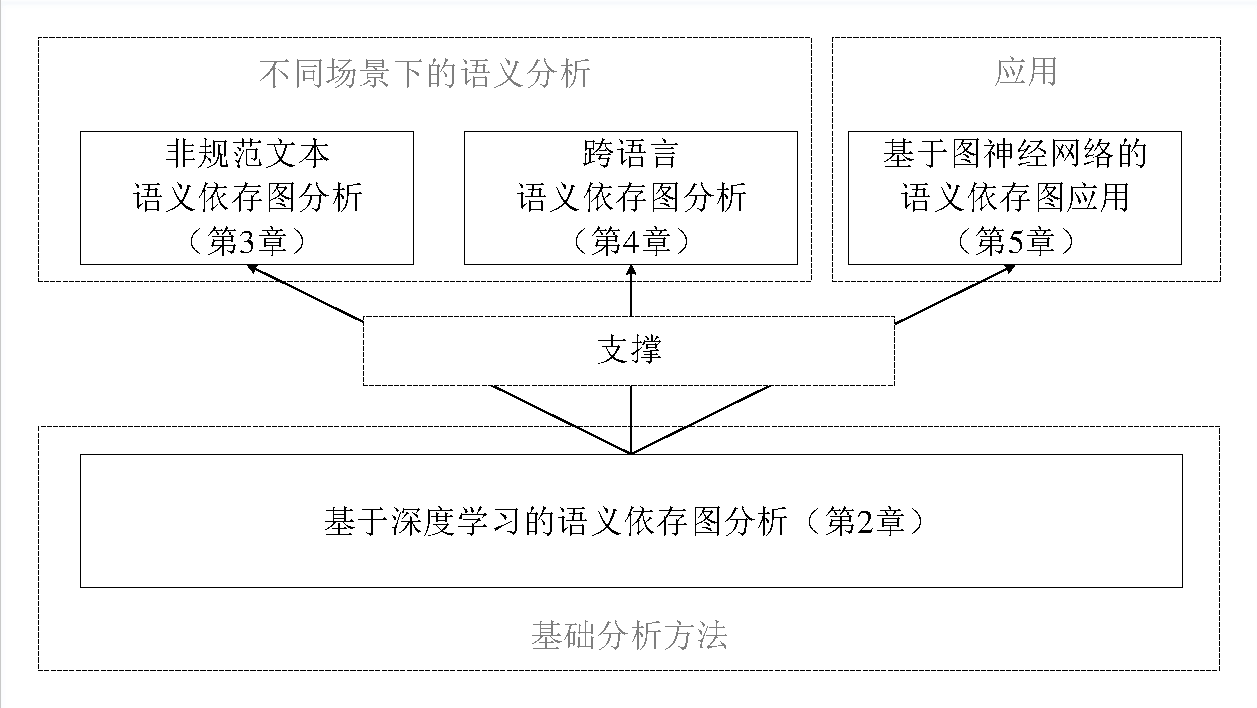
\includegraphics[width=0.95\textwidth]{figures/section_relation.pdf}
    %\caption{论文总体框架}[Structure of the thesis]
    \bicaption[fig:section-relation]{}{论文总体框架}{Fig.$\!$}{Structure of the thesis}
    \label{}
\end{figure}

论文结构框架如图\ref{fig:section-relation}所示,具体来说,本文共包含5章,各章内容组织如下:

在第1章中,本文介绍了中文语义依存图分析的研究背景与意义,并对语义依存图分析的研究现状进行了概述与分析,最后对本文主要内容进行了规划。

在第2章中,针对图结构依存分析的挑战,本文使用基于转移的分析方法,设计了一套用于生成依存图的转移系统,并使用基于栈-长短时记忆网络的模型根据当前转移状态预测下一个转移动作。实验结果表明,本文提出的语义依存图分析方法相比此前的方法取得了显著的性能提升。

在第3章中,针对语义依存图分析在非规范文本上性能远低于规范文本的问题,本文首先设计了一套针对语义依存图分析的对抗样本攻击框架,用于生成使目标语义依存图分析器性能下降的非规范文本。
接着,本文深入探究了对此类非规范文本特征和不同类型分析器的鲁棒性,并在此基础上分别提出了基于对抗样本训练和基于模型融合的方法用于提升现有的依存图分析器的鲁棒性。
实验结果表明,本文提出的对抗样本攻击框架能生成高质量的非规范文本,在它们的帮助下本文有效提升了现有的基于神经网络的依存图分析器的鲁棒性。

在第4章中,针对目前世界上大部分语言上语义依存图语料稀缺,语义依存图分析困难的问题,本文首先对中文语义依存图标注规范进行修改,使其适应多语言场景。
接着,本文提出基于标签转换和图神经网络的方法,首先利用标签转换将现有的多语言大规模通用句法依存语料转换为语义依存图的伪数据,然后使用这些数据和小规模人工标注的语义依存图训练基于图神经网络的编码-解码模型,实现将句法依存语料自动转化为语义依存图语料。
最后,本文使用这些自动转化的语义依存图语料训练跨语言的语义依存图分析器。
实验结果表明,本文提出的跨语言语义依存图分析方法相比于普通的只使用跨语言词向量的方法取得了显著的性能提升。

在第5章中,针对语义依存图分析的应用问题,结合中文的词具有字级别的内部结构的特点,本文提出了基于字级别图结构神经网络编码器,将中文语义依存图融合到预训练模型中,从而增强其表示能力。
本文接着使用这种增强的预训练模型获取的词表示作为其他自然语言处理任务的输入,从而提升其性能。
实验结果表明,本文提出的方法显著提升了语义角色标注和关系抽取任务的性能。

% Local Variables:
% TeX-master: "../thesis"
% TeX-engine: xetex
% End:
% !Mode:: "TeX:UTF-8"

\chapter[基于深度学习的语义依存图分析]{基于深度学习的语义依存图分析}[Semantic Dependency Graph Parsing Based on Deep Learning]

\section{引言}[Introduction]

在过去的二十几年中,自然语言处理领域涌现出了大量的关于树结构的句法分析的研究工作\cite{eisner-1996-three, nivre-2004-incrementality, mcdonald-etal-2006-online, nivre-2009-non, zhang-nivre-2011-transition}。
近年来,在神经网络模型的帮助下,句法依存分析的准确率取得了显著的提升\cite{chen-manning-2014-fast,weiss-etal-2015-structured, andor-etal-2016-globally}。
然而,当表示的目标从句法结构变为深层语义结构时,树结构的不足之处就展现了出来。
从语义层面上来说,句子中的一个词可以同时作为多个谓词(predicate)的论元(argument)。
为了刻画这种语义关系,有研究者使用了有向无环图(a directed acyclic graph,简称DAG)结构,其中的节点允许有多条入弧。
Oepen等人\cite{oepen-etal-2015-semeval}于2015年公布了Broad-Coverage Semantic Dependency Graph语料库,包含了英文、捷克语和中文上的三种语义依存图标注。
而Che等人\cite{che-etal-2016-semeval}于2016年公布了中文语义依存图语料库。
本文重点研究的就是其中的中文语义依存图的分析技术及应用。

正如第\ref{sec:sdp}节所介绍,图结构的引入在提升语义表示能力的同时,也因其中每个词父节点数量的不确定性给依存图分析带来了巨大的挑战。
虽然语义依存图的分析方法可以从其前身——句法依存树分析的工作中寻找灵感,但如何生成多父节点词,是所有的依存图分析方法都无法回避的,也是依存图分析中的核心问题。
除此之外,此前的语义依存图分析模型,大部分仍然在使用传统的基于特征工程的统计机器学习方法。
然而自从Chen等人\cite{chen-manning-2014-fast}于2014年首次将神经网络模型引入基于转移的句法依存分析器中,神经网络模型已经在依存分析领域证明了其强大的特征表示能力。
但该方法仍然使用了人工设计的特征,没有完全避免需要专家知识的特征工程。

总的来说,想要实现高效、准确的语义依存图分析模型需要面临两个挑战:

1.如何解决多父节点词的问题?

2.如何更高效、准确地实现分析模型的学习?

针对上述第一个问题,本章采用了基于转移的分析方法,设计了一套用于生成依存图的转移系统,使其在不需要预处理和后处理的情况下能够直接根据输入的句子完整地生成其对应的语义依存图。

针对上述第二个问题,本章采用了基于栈-长短时记忆网络(Stack-LSTM)的模型,用LSTM分别获取转移系统中各个部分的上下文相关表示向量,组成当前转移状态的表示向量,并用其预测下一个转移动作。
特别的,本章为转移系统中重要的队列和已经生成的子图分别使用了双向LSTM相减模块和递增的Tree-LSTM模块来更好地获取其表示。

本章在前文介绍的中文和英文的语义依存图语料库上分别测试了上述模型,实验结果表明,本章提出的语义依存图分析方法在此前方法的基础上取得了显著的性能提升。

\section{背景与相关工作}[Related Work]
\label{sec:chapter2-related-work}

基于转移的依存分析主要由转移系统和转移动作分类器两部分组成。
其中转移系统包括了由列表、栈等结构组成的环境和一系列预定义的对环境进行改变的转移动作。
包括列表、栈等结构在内的所有环境在某一时间节点的情况称为转移状态。
转移动作在执行时不仅修改转移状态,也会同时生成词之间的依存弧,而目标依存结构就是通过一系列的转移动作生成的。
本文第\ref{sec:syntactic-dependency-parsing}节已经介绍了标准弧转移系统并简要介绍了基于转移的分析模型中的转移动作分类器。
本节将重点介绍与本章研究内容密切相关的贪心弧转移系统(Arc-Eager Transition System)\cite{choi-palmer-2011-getting,choi-mccallum-2013-transition}和Stack-LSTM模型结构\cite{dyer-etal-2015-transition}。

Choi等人\cite{choi-palmer-2011-getting}于2011年提出了一种贪心弧转移算法。
从转移动作上来说,该算法与标准弧转移算法的主要区别是标准弧转移算法生成的是栈顶的两个词之间的依存关系,而贪心弧转移算法生成的是栈顶词和列表中第一个词之间的依存关系。
这种生成弧的顺序无法保证一个词找到其父节点时其所有子节点都已经提前找到,为了解决这一问题,该算法里又增加了规约(Reduce)和跳过(PASS)动作。
其中规约动作用于处理所有入弧和出弧都已经找到的节点,将其从转移状态中删除。
有了规约动作,原来生成弧的动作,即左弧(Left)和右弧(Right)将不再承担删除子节点的任务。
而跳过动作则暂时将栈顶词弹出,从而允许列表中的词与栈中其他词之间生成弧。
而为了保存栈顶弹出的词,该算法的转移状态中在一般的栈和列表的基础上额外增加了一个双向队列,专门保存这些被弹出的词,等到下一个移进动作时一起再移入栈中。

从另一个角度来说,这种转移动作的设计实际上是通过将生成弧的动作与删除词的动作分离来解决贪心弧转移算法的劣势,即生成弧的时候无法保证该弧指向的子节点的所有子节点都已经找到。
然而这种转移动作的分离又引入了一个新的问题。
基于转移的依存分析方法中,转移动作分类器通过当前转移状态来预测下一个要执行的转移动作,这就要求每个转移动作执行之后会对转移状态进行明显的修改。
然而由于生成弧的动作不再删除子节点,其对转移状态的改变很小(只是在已生成的子图中加了一条弧),难以被分类器察觉。
为了解决这一问题,Choi等人对生成弧的动作(包括左弧、右弧和不生成弧)和修改转移状态的动作(移进、规约等)进行了组合,确保每个生成弧的动作都会对转移状态进行修改。

\begin{table}[htbp]
    \bicaption[tbl:choi-transition-actions]{}{List-Based Arc-Eager转移算法中的转移动作集合}{Table$\!$}{Transition actions in List-Based Arc-Eager transition algorithm.}
	\vspace{0.5em}\centering\wuhao
	\begin{tabular}{lll}
		\toprule[1.5pt]
		转移动作 \ \ \ \ & 当前转移状态 & $\Rightarrow$ 下一转移状态 \\
		\midrule[1pt]
		Left$_l$-Reduce &\ \ $([\sigma|i],\,\delta,\,[j|\beta],\,E)$ & $\Rightarrow (\sigma,\,\delta,\,[j|\beta],\,E\,\cup\,\{(i\xleftarrow{l}j)\})$ \\
		Right$_l$-Shift &\ \ $([\sigma|i],\,\delta,\,[j|\beta],\,E)$ & $\Rightarrow ([\sigma|i|\delta|j],\,[\ ],\,\beta,\,E\,\cup\,\{(i\xrightarrow{l}j)\})$ \\
		No-Shift &\ \ $([\sigma|i],\,\delta,\,[j|\beta],\,E)$ & $\Rightarrow 
		([\sigma|i|\delta|j],\,[\ ],\,\beta,\,E)$ \\
		No-Reduce &\ \ $([\sigma|i],\,\delta,\,[j|\beta],\,E)$ & $\Rightarrow (\sigma,\,\delta,\,[j|\beta],\,E)$\\
		%\hline
		Left$_l$-Pass &\ \ $([\sigma|i],\,\delta,\,[j|\beta],\,E)$ & $\Rightarrow (\sigma,\,[i|\delta],\,[j|\beta],\,E\,\cup\,\{(i\xleftarrow{l}j)\})$\\
		Right$_l$-Pass &\ \ $([\sigma|i],\,\delta,\,[j|\beta],\,E)$ & $\Rightarrow (\sigma,\,[i|\delta],\,[j|\beta],\,E\,\cup\,\{(i\xrightarrow{l}j)\})$\\
		No-Pass &\ \ $([\sigma|i],\,\delta,\,[j|\beta],\,E)$ & $\Rightarrow (\sigma,\,[i|\delta]	,\,[j|\beta],\,E)$\\
		\bottomrule[1.5pt]
	\end{tabular}
\end{table}

他们将该算法命名为基于列表的贪心弧(List-Based Arc-Eager)转移算法,其中定义的转移动作如表\ref{tbl:choi-transition-actions}所示。
表中$\sigma$,$\delta$和$\beta$分别代表上文介绍的转移系统中的栈、双向队列和列表。
而$E$表示算法生成的所有依存弧集合。

值得注意的是,将生成弧的动作和删除词的动作进行分离的思想,虽然在该工作中是为了弥补贪心弧转移算法的劣势,但对于语义依存图的生成也有重要意义。
利用这种思想可以设计出适用于依存图生成的转移系统,在为句中词找到一个父节点的时候不立即将其从转移状态中删除,而是继续寻找它的其他父节点,直到一个词的所有父节点都已找到再对其进行规约。
因此,本章选择在List-Based Arc-Eager转移算法的基础上设计语义依存图的转移算法。

% stack-lstm
Chen等人\cite{chen-manning-2014-fast}于2014年首次将多层感知器(
Multi-Layer Perceptron,简称MLP)引入基于转移的依存分析器,利用其强大的表示能力显著提高了句法依存分析的性能。
但该方法仍然受限于传统特征工程的思想,使用了固定位置的隐层表示作为转移状态的表示,用于预测下一个转移动作。
尽管如此,该方法开启了基于神经网络模型的句法依存分析的大门,启发了此后很多的相关工作。

Dyer等人\cite{dyer-etal-2015-transition}于2015年提出了使用Stack-LSTM代替MLP,从而全自动地获取转移状态表示的方法。
具体来说,假设$\bm{x}_t$是$t$时刻的输入向量,普通的LSTM在$t$时刻首先计算控制信息的输入门$\bm{i}_t$(Input Gate)、遗忘门$\bm{f}_t$(Forget Gate)和保存信息的记忆单元$\bm{c}_t$(Memory Cell):
\begin{equation}
    \bm{i}_t = \sigma(\bm{W}_{ix}\bm{x}_t + \bm{W}_{ih}\bm{h}_{t-1} + \bm{W}_{ic}\bm{c}_{t-1} + \bm{b}_i)
\end{equation}
\begin{equation}
    \bm{f}_t = \sigma(\bm{W}_{fx}\bm{x}_t + \bm{W}_{fh}\bm{h}_{t-1} + \bm{W}_{fc}\bm{c}_{t-1} + \bm{b}_f)
\end{equation}
\begin{equation}
    \bm{c}_t = \bm{f}_{t}\odot\bm{c}_{t-1} + \bm{i}_{t}\odot \tanh(\bm{W}_{cx}\bm{x}_{t} + \bm{W}_{ch}\bm{h}_{t-1} + \bm{b}_c)
\end{equation}
其中$\odot$表示逐点乘积(Hadamard product),$\sigma$表示非线性变换函数,例如sigmoid或tanh。
之后计算控制LSTM输出的输出门$\bm{o}_t$(Output Gate)并用其计算时刻$t$的隐层输出$\bm{h}_t$:
\begin{equation}
    \bm{o}_t = \sigma(\bm{W}_{ox}\bm{x}_t + \bm{W}_{oh}\bm{h}_{t-1} + \bm{W}_{oc}\bm{c}_{t-1} + \bm{b}_o)
\end{equation}
\begin{equation}
    \bm{h}_t = \bm{f}_{t}\odot\tanh(\bm{c}_{t})
\end{equation}
通过上述三种门的控制和记忆单元,LSTM能够更新、储存和重置较长序列的信息,从而解决长距离依赖问题。

LSTM的特性使其很适合用于抽取基于转移的依存分析器中转移系统各个部分的信息。
然而普通的LSTM只能建模从左到右或从右到左的序列。
而在基于转移的依存分析中,转移系统中的栈中的词是不断变化的,这种变化不仅有单方向的增加,也有删除。
为了解决该问题,Dyer等人提出了Stack-LSTM模型,在普通LSTM中加入一个栈指针,永远指向当前栈顶词。
在从栈中删除栈顶词时,指针指向新的栈顶词。
在向栈中移入新的词时,由栈指针指向的那个词提供LSTM计算所需的$\bm{c}_{t-1}$和$\bm{h}_{t-1}$。
通过这种方式,他们将LSTM成功应用于基于转移的依存分析,实现了全自动的获取当前转移状态的表示,而不需要任何人工定义特征。

本章的提出的语义依存图分析器建立在Stack-LSTM的基础上,并提出了两种神经网络模块,用于更好地获取转移系统中队列和已经生成的子图的表示。


\section{基于转移的语义依存图分析方法}[Transition-Based Semantic Dependency Graph Parsing]

正如第\ref{sec:chapter2-related-work}节所介绍,List-Based Arc-Eager算法中将生成弧的动作和删除词的动作分离的思想,对于依存图的生成也有重要借鉴意义。
因此,为了设计适用于依存图结构的分析器,本章选择了基于转移的分析方法作为突破口,并在List-Based Arc-Eager算法的基础上设计适用于语义依存图生成转移系统。
对于基于转移的分析方法中另一个重要的部分——转移动作分类器,本章选择Stack-LSTM作为基础模型,从而完全摆脱了需要专家知识的特征工程,并为转移系统中重要的保存待处理词的列表和系统中部分生成的子图分别提出了双向LSTM相减模块和递增的Tree-LSTM模块,用以更好地获取其表示。
本节将从转移系统和基于Stack-LSTM的依存图分析器模型结构两方面具体介绍本章提出的语义依存图分析器。
%这类方法通过执行一系列从初始转移状态到终止转移状态的移进、规约等转移动作,实现目标结构的生成。这类方法由两个重要部分组成,一是转移系统,它定义了存放句中词的结构、转移动作集合以及转移动作执行的规则;二是分类器,它以当前转移状态为依据,预测出下一步要执行的转移动作。基于转移的分析方法的核心就是训练一个好的分类器,使得当我们按照它预测的动作产生语义依存图时,与正确的语义依存图尽可能相似。接下来分别介绍我们实现的用于分析语义依存图的转移系统和分类器。

\subsection{转移系统}[Transition System]

%由于语义依存图具有非投射性(弧之间存在交叉),在设计转移系统时,我们参考了Choi等人提出的用于分析非投射依存树的转移系统,\cite{choi-palmer:2011:ACL-HLT2011,choi-mccallum:2013:ACL2013}并对其做了改进,使其能够直接分析语义依存图。
为了处理语义依存图中多父节点词的生成问题,本章在List-Based Arc-Eager算法的基础上设计适用于依存图分析的转移系统。
主要思想是在找到一个词的父节点之后,不再马上将其从转移系统中删除(由于在树结构中,一个词只有一个父节点,因此在分析依存树时,一旦找到了一个词的父节点,就会立即将其从转移系统中删除),而是仍然将其保存在系统中,这样未来这个词就能找到其它的父节点。
要实现这一目的,主要需要对转移系统中各转移动作的执行条件进行更改。
具体来说,基于转移的分析方法的训练过程中首先需要按照预定义的执行条件及正确的语义依存图生成神谕(oracle)转移动作序列。
神谕转移动作序列是一条从初始转移状态一直到终结转移状态的序列,在执行过程中生成正确的语义依存图。
其作用是生成一系列的由当前转移状态到下一步的转移动作的二元组,其中当前转移状态作为输入,下一步转移状态作为输出来训练转移动作分类器。
在预测过程中,该模型从初始状态开始,每一步使用训练好的转移动作分类器预测下一个转移动作并执行,直到遇到终结状态为止,这时就完成了输入句子语义依存图的预测。

接下来给出该转移系统的正式定义:本章用一个四元组$(\sigma,\delta,\beta,E)$来表示任意一个转移状态,其中$\sigma$是用于保存正在处理中的词的栈(Stack);
$\delta$是用于保存从$\sigma$中弹出的词的双向队列(Deque),这些词在将来某一时刻将被重新压入$\sigma$中;
$\beta$是用于保存等待处理的词的列表(List);
$E$用于保存已经生成的依存弧。
为了简洁,这里用$i$表示第$i$个词$w_i$,其中$0$表示虚拟根节点$w_0$,根据定义,每个依存图的根节点只有一个子节点。
初始转移状态是$([0],[\ ],[1,\dots,n],\emptyset)$,表示栈中保存虚拟根节点,而需要分析的句子中的所有词保存在列表中,$\delta$和$E$为空。
终结转移状态是$(\sigma,[\ ],[\ ],E)$,表示$\beta$和$\delta$为空,而$E$中保存的是生成的语义依存图中的所有弧。
另外,$(i\xrightarrow{l} j)$表示一条从$w_i$指向$w_j$的依存弧,其依存关系为$l$。$(i\rightarrow j)$和$(i\rightarrow^*j)$分别表示$w_i$是$w_j$的父节点和祖先节点。
在分析过程中,依存弧只会在栈$\sigma$的顶部元素$w_i$和列表$\beta$的第一个元素$w_j$之间生成。在训练过程中,转移动作通过标准语义依存图生成,在解码过程中,转移动作通过神经网络分类器预测产生。

\begin{table}[h]
    \bicaption[tbl:preconditions]{}{依存树分析算法与依存图分析算法转移动作执行条件对比}{Table$\!$}{Preconditions of Transitions for tree and graph parsing respectively.}
    \vspace{0.5em}\centering\wuhao
	\begin{tabular}{lL{16em}L{16em}}
		\toprule[1.5pt]
		\multirow{2}{*}{动作} & \multicolumn{2}{c}{List-Based Arc-Eager算法中转移动作的执行条件} \\
		\cline{2-3}
		& 依存树分析 & 依存图分析 \\
		\midrule[1pt]
		\multirow{2}{*}{Left-$*$} & $[i\neq0] \wedge \neg[(i\rightarrow ^*j)\in E]$ & \multirow{2}{*}{$[i\neq0] \wedge \neg[(i\rightarrow ^*j)\in E] $} \\
		& $\wedge \neg[\exists k.(i\leftarrow k)\in E] $ & \\
		Right-$*$ & $\neg[(j\rightarrow ^*i)\in E] \wedge \neg[\exists k.(k\rightarrow j)\in E] $ & $\neg[(j\rightarrow ^*i)\in E]$ \\
		\multirow{2}{*}{$*$-Reduce} & $[\exists h.(h\rightarrow i)\in E]$  & $[\exists h.(h\rightarrow i)\in E]$ \\
		& $\wedge \neg[\exists k\in\beta.(i\rightarrow k)]$ & $\wedge \neg[\exists k\in\beta.(i\rightarrow k)\vee(i\leftarrow k)]$ \\
		$*$-Shift & \multicolumn{2}{c}{ $\neg[\exists k\in \sigma.(k\neq i) \ \wedge ((k\rightarrow j)\vee(k\leftarrow j))]$ } \\
		\bottomrule[1.5pt]
	\end{tabular}
\end{table}

为了实现对依存图的分析,本章List-Based Arc-Eager算法中的转移动作的执行条件进行修改。
这些执行条件是用于生成训练过程中的神谕转移动作序列的,在转移系统中十分重要,因为它们决定了一套转移系统能生成什么样的目标结构。
原始的针对依存树的转移动作执行条件和新的针对依存图的执行条件如表\ref{tbl:preconditions}所示,其中的$i$和$j$分别表示栈顶词和列表中的第一个词。
Left-$*$和Right-$*$分别表示以Left和Right开头的动作,$*$-Reduce和$*$-Shift分别表示以Reduce和Shift结尾的动作。
执行条件主要分为两部分,分别是以生成弧的动作(左弧或右弧)为开头的转移动作的条件和以改变转移状态的动作(移进或规约)为结尾的转移动作的条件。
对于前者,在原始的依存树分析系统中,要求生成的依存弧指向的子节点不为虚拟根节点,且在已经生成的弧中,不存在一条由当前子节点到当前父节点的路径(这一点是为了保证生成的结构中不存在环)。
此外,依存树分析中还要求已经生成的弧中不存在当前的子节点的父节点,这是为了保证依存树中每个词只有一个父节点。
而在新的依存图分析系统中,为了允许一个词有多个父节点,则删除了这一条件。
对于后者,在依存树分析系统中,移进的条件是栈中没有任何词与当前列表中第一个词之间有弧,这一条件在依存图分析系统中保留。
而依存树分析系统中规约的条件是当前栈顶词已找到一个父节点,且在列表中的所有词中,不存在当前栈顶词的子节点。
在新的依存图分析系统中,除了要保证栈顶词所有的子节点都已找到,还要保证其所有的父节点都已找到,才能将其从系统中规约掉。

\begin{figure}[h]
	\centering
	\begin{dependency}[theme = simple,label style={font=\bfseries,thick}]
		\begin{deptext}[column sep=0.5em]
			他$_1$ \& 太$_2$ \& 小气$_3$ \& ,$_4$ \& 不$_5$ \& 肯$_6$ \& 请$_7$ \& 我们$_8$ \& 吃饭$_9$ \\
		\end{deptext}
		\deproot{3}{ROOT$_0$}
		\depedge[edge style={red, dashed}, label style={text=red}]{3}{1}{Exp}
		\depedge{3}{2}{mDegr}
		\depedge{3}{4}{mPunc}
		\depedge{3}{7}{eCau}
		\depedge[edge start x offset=6pt, style={red, dashed}, label style={text=red}]{7}{1}{Agt}
		\depedge{6}{5}{mNeg}
		\depedge{7}{6}{mMod}
		\depedge[edge style={red, dashed}, label style={text=red}]{7}{8}{Datv}
		\depedge{7}{9}{ePurp}
		\depedge[edge style={red, dashed}, label style={text=red}]{9}{8}{Agt}
	\end{dependency}
	\bicaption[fig:chapter2-sdg-example]{}{中文语义依存图实例}{Fig.$\!$}{Example of Chinese semantic dependency graph}
\end{figure}


\begin{table*}[thbp]
    \bicaption[tbl:transition-sequence-example]{}{用List-Based Arc-Eager算法获得的图\ref{fig:chapter2-sdg-example}对应的神谕转移动作序列}{Table$\!$}{Oracle transition sequence of Fig.\ref{fig:chapter2-sdg-example} generated by List-Based Arc-Eager algorithm.}
    \vspace{0.5em}\centering\wuhao
	\begin{tabular}{C{3em}L{7em}R{4.5em}C{4em}L{4em}L{9em}}
		\toprule[1.5pt]
		状态 & 转移动作 & $\sigma$ & $\delta$ & $\beta$ & $E$ \\
		\midrule[1pt]
		$0$ & Initialization & $[0]$ & $[\ ]$ & $[1, \dots, 9]$ & $\emptyset $ \\
		$1$ & No-Shift & $[0, 1]$ & $[\ ]$ & $[2, \dots, 9]$ &  \\
		$2$ & No-Shift & $[0, 1, 2]$ & $[\ ]$ & $[3, \dots, 9]$ &  \\
		$3$ & Left-Reduce & $[0, 1]$ & $[\ ]$ & $[3, \dots, 9]$ & $E\ \cup\ \{2\xleftarrow{\textrm{mDegr}}3\}$ \\
		$4$ & Left-Pass & $[0]$ & $[1]$ & $[3, \dots, 9]$ & $E\ \cup\ \{1\xleftarrow{\textrm{Exp}}3\}$ \\
		$5$ & Right-Shift & $[0, 1, 3]$ & $[\ ]$ & $[4, \dots, 9]$ & $E\ \cup\ \{0\xrightarrow{\textrm{ROOT}}3\}$ \\
		$6$ & Right-Shift & $[0, 1, 3, 4]$ & $[\ ]$ & $[5, \dots, 9]$ & $E\ \cup\ \{3\xrightarrow{\textrm{mPunc}}4\}$ \\
		$7$ & No-Reduce & $[0, 1, 3]$ & $[\ ]$ & $[5, \dots, 9]$ &  \\
		$8$ & No-Shift & $[0, 1, 3, 5]$ & $[\ ]$ & $[6, \dots, 9]$ &  \\
		$9$ & Left-Reduce & $[0, 1, 3]$ & $[\ ]$ & $[6, \dots, 9]$ & $E\ \cup\ \{5\xleftarrow{\textrm{mNeg}}6\}$ \\
		$10$ & No-Shift & $[0, 1, 3, 6]$ & $[\ ]$ & $[7, 8, 9]$ &  \\
		$11$ & Left-Reduce & $[0, 1, 3]$ & $[\ ]$ & $[7, 8, 9]$ & $E\ \cup\ \{6\xleftarrow{\textrm{mMod}}7\}$ \\
		$12$ & Right-Pass & $[0, 1]$ & $[3]$ & $[7, 8, 9]$ & $E\ \cup\ \{3\xrightarrow{\textrm{eCau}}7\}$ \\
		$13$ & Left-Reduce & $[0]$ & $[3]$ & $[7, 8, 9]$ & $E\ \cup\ \{1\xleftarrow{\textrm{Agt}}7\}$ \\
		$14$ & No-Shift & $[0, 3, 7]$ & $[\ ]$ & $[8, 9]$ &  \\
		$15$ & Right-Shift & $[0, 3, 7, 8]$ & $[\ ]$ & $[9]$ & $E\ \cup\ \{7\xrightarrow{\textrm{Datv}}8\}$ \\
		$16$ & Left-Reduce & $[0, 3, 7]$ & $[\ ]$ & $[9]$ & $E\ \cup\ \{8\xleftarrow{\textrm{Agt}}9\}$ \\
		$17$ & Right-Shift & $[0, 3, 7, 9]$ & $[\ ]$ & $[\ ]$ & $E\ \cup\ \{7\xrightarrow{\textrm{ePurp}}9\}$ \\
		\bottomrule[1.5pt]
	\end{tabular}
\end{table*}

\iffalse
\begin{table*}[thbp]
    \bicaption[tbl:transition-sequence-example]{}{用List-Based Arc-Eager算法获得的图\ref{fig:chapter2-sdg-example}对应的神谕转移动作序列}{Table$\!$}{Oracle transition sequence of Fig.\ref{fig:chapter2-sdg-example} generated by List-Based Arc-Eager algorithm.}
    \vspace{0.5em}\centering\wuhao
	%\centering
	\small
	\renewcommand{\arraystretch}{1.2}
	\begin{tabular}{C{3em}L{7em}R{4.5em}C{4em}L{4em}L{9em}}
		\hline
		\bf 状态 & \bf 转移动作 & $\sigma$ & $\delta$ & $\beta$ & $E$ \\
		\hline
		$0$ & Initialization & $[0]$ & $[\ ]$ & $[1, \dots, 9]$ & $\emptyset $ \\
		$1$ & No-Shift & $[0, 1]$ & $[\ ]$ & $[2, \dots, 9]$ &  \\
		$2$ & No-Shift & $[0, 1, 2]$ & $[\ ]$ & $[3, \dots, 9]$ &  \\
		$3$ & Left-Reduce & $[0, 1]$ & $[\ ]$ & $[3, \dots, 9]$ & $E\ \cup\ \{2\leftarrow \textrm{mDegr}-3\}$ \\
		$4$ & Left-Pass & $[0]$ & $[1]$ & $[3, \dots, 9]$ & $E\ \cup\ \{1\leftarrow \textrm{Exp}-3\}$ \\
		$5$ & Right-Shift & $[0, 1, 3]$ & $[\ ]$ & $[4, \dots, 9]$ & $E\ \cup\ \{0- \textrm{ROOT}\rightarrow 3\}$ \\
		$6$ & Right-Shift & $[0, 1, 3, 4]$ & $[\ ]$ & $[5, \dots, 9]$ & $E\ \cup\ \{3- \textrm{mPunc}\rightarrow 4\}$ \\
		$7$ & No-Reduce & $[0, 1, 3]$ & $[\ ]$ & $[5, \dots, 9]$ &  \\
		$8$ & No-Shift & $[0, 1, 3, 5]$ & $[\ ]$ & $[6, \dots, 9]$ &  \\
		$9$ & Left-Reduce & $[0, 1, 3]$ & $[\ ]$ & $[6, \dots, 9]$ & $E\ \cup\ \{5\leftarrow \textrm{mNeg}-6\}$ \\
		$10$ & No-Shift & $[0, 1, 3, 6]$ & $[\ ]$ & $[7, 8, 9]$ &  \\
		$11$ & Left-Reduce & $[0, 1, 3]$ & $[\ ]$ & $[7, 8, 9]$ & $E\ \cup\ \{6\leftarrow \textrm{mMod}-7\}$ \\
		$12$ & Right-Pass & $[0, 1]$ & $[3]$ & $[7, 8, 9]$ & $E\ \cup\ \{3- \textrm{eCau}\rightarrow 7\}$ \\
		$13$ & Left-Reduce & $[0]$ & $[3]$ & $[7, 8, 9]$ & $E\ \cup\ \{1\leftarrow \textrm{Agt}-7\}$ \\
		$14$ & No-Shift & $[0, 3, 7]$ & $[\ ]$ & $[8, 9]$ &  \\
		$15$ & Right-Shift & $[0, 3, 7, 8]$ & $[\ ]$ & $[9]$ & $E\ \cup\ \{7- \textrm{Datv}\rightarrow 8\}$ \\
		$16$ & Left-Reduce & $[0, 3, 7]$ & $[\ ]$ & $[9]$ & $E\ \cup\ \{8\leftarrow \textrm{Agt}-9\}$ \\
		$17$ & Right-Shift & $[0, 3, 7, 9]$ & $[\ ]$ & $[\ ]$ & $E\ \cup\ \{7- \textrm{ePurp}\rightarrow 9\}$ \\
		\hline
	\end{tabular}
\end{table*}
\fi

为了具体说明上述的依存图转移系统的工作方式,接下来给出一个由该系统生成语义依存图的例子。
图\ref{fig:chapter2-sdg-example}是一个中文语义依存图实例,表\ref{tbl:transition-sequence-example}给出了使用上述转移系统生成该语义依存图的正确转移动作序列。

需要重点注意的是图\ref{fig:chapter2-sdg-example}中红色虚线表示的弧,正是这些弧引入了多父节点情况。
具体来说,在状态4时,转移系统用Left-Pass动作生成$w_3$(小气)指向$w_1$(他)的依存弧,但由于$w_1$(他)在$\beta$中还有另一个父节点$w_7$(请),它被从$\sigma$中暂时移入$\delta$。
经过一系列转移动作,在状态12时,由于$w_7$(请)在$\sigma$中还有一个子节点$w_1$(他),因此系统执行了Right-Pass动作而不是Right-Shift动作。该动作将$w_3$(小气)移入$\delta$从而允许$w_7$(请)和$w_1$(他)之间产生一条弧。
紧接着在状态13时,系统用Left-Reduce生成了由$w_7$(请)指向$w_1$(他)的依存弧。
此时由于$w_1$(他)的所有父节点和子节点都已经找到,该词被从转移状态中规约掉。
通过这一系列转移动作,该系统解决了句中“他”这个词同时有两个父节点“小气”和“请”的情况。
类似地,为了解决句中词“我们”同时有两个父节点“请”和“吃饭”的情况,在状态15和状态16时,系统先用Right-Shift动作生成了由$w_7$(请)指向$w_8$(我们)的弧,并且没有将其中的子节点删除,然后再用Left-Reduce动作生成了由$w_9$(吃饭)指向$w_8$(我们)的弧。
这是由于$w_8$(我们)的所有父节点和子节点都已找到,该词被从转移状态中规约掉。


\subsection{基于栈-长短时记忆网络的依存图分析模型}[Dependency Graph Model Based on Stack-LSTM Networks]

如果说转移系统是基于转移的分析方法的骨架,那么分类器就是它的大脑,负责以当前的转移状态为依据决定下一步要执行的转移动作。
传统的基于转移的依存分析方法,无论是以图结构为目标的\cite{sagae-tsujii-2008-shift,titov-etal-2009-online},还是以树结构为目标的\cite{yamada-etal-2003-statistical,nivre-2004-incrementality}普遍使用的都是基于特征工程的传统统计及其学习方法。
这类方法普遍使用百万级别的高维稀疏人工定义特征(例如用01特征函数表示一个特征是否存在),不但需要人类专家知识,还会导致数据稀疏问题。

本章使用的转移系统分类器建立在第\ref{sec:chapter2-related-work}节介绍的Stack-LSTM模型结构基础上。
在Stack-LSTM中,几个单向LSTM分别被用于计算转移系统中每部分所有信息的表示向量,然后这些向量被组合起来作为当前转移状态的表示$\bm{e}_t$:

\vspace{-0.6em}
\begin{equation}
	\label{eq:trans}
	\bm{e}_t=\max(0,W[\bm{s}_t;\bm{b}_t; \bm{p}_t; \bm{a}_t ]+\bm{d})
\end{equation}

其中$W$是参数矩阵,$\bm{s}_t$是Stack-LSTM对$\sigma$的编码,$\bm{b}_t$是Stack-LSTM对$\beta$的编码, $\bm{p}_t$是Stack-LSTM对$\delta$的编码,$\bm{a}_t$是Stack-LSTM对历史转移动作序列$A$的编码,$\bm{d}$是偏置项。
之后转移状态$\bm{e}_t$用于计算该状态下转移动作的概率分布:

\vspace{-0.6em}
\begin{equation}
	\label{eq:trans-softmax}
	p(z_t|e_t)=\frac{\exp(\bm{g}^T_{z_t}\bm{e}_t + q_{z_t})}{\sum_{z'\in A(\sigma, \beta)}\exp (\bm{g}^T_{z'}\bm{e}_t+q_{z'})}
\end{equation}

其中$\bm{g}_z$是用于表示转移动作$z$的列向量,而$q_z$是其偏置项,集合$A(\sigma,\beta)$是在当前状态下可以执行的转移动作。

为了获取对转移状态更全面的表示,本章在该结构的基础上提出了2个有效的神经网络模块,即双向LSTM相减模块(Bi-LSTM Subtraction,简称BS)和递增的Tree-LSTM模块(Incremental Tree-LSTM,简称IT),分别对转移过程中的列表和子图进行建模,最终的依存图分析系统简称为BS-IT系统。
图\ref{fig:bs-it}给出了本章提出的模型的整体结构图。接下来分别对两个模块进行具体介绍。

\begin{figure}[hbtp]
	\centering
	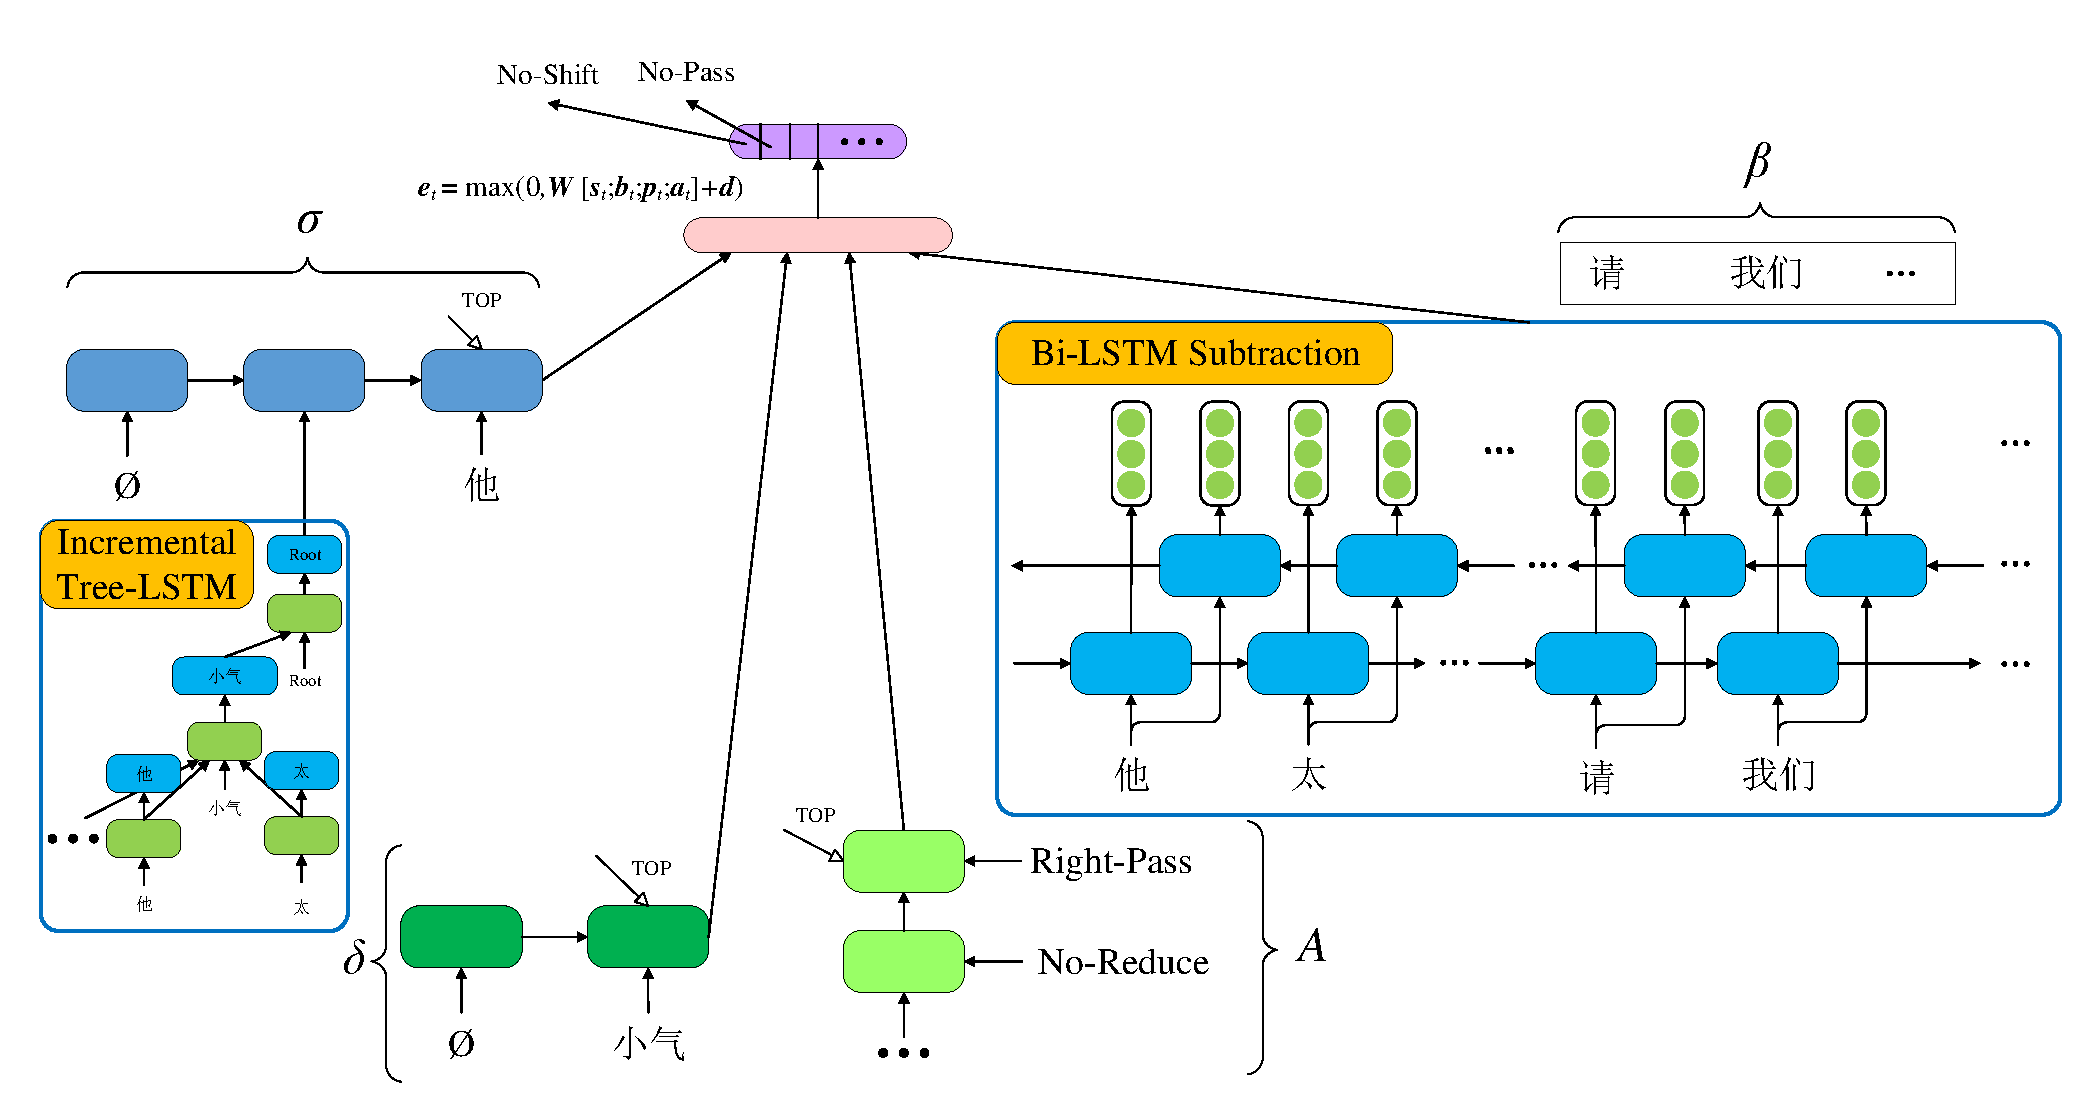
\includegraphics[width=0.9\textwidth]{figures/bs-it.pdf}
	\bicaption[fig:bs-it]{}{BS-IT系统模型整体结构图}{Fig.$\!$}{Model structure of BS-IT system}
\end{figure}

原始的Stack-LSTM中简单地使用从右向左的单向LSTM的最后一个隐层状态向量表示列表中的所有信息。
这种方法不但无法获取列表之外的词(已被移入栈中或规约)的信息,也损失了从左向右的上下文信息。
而且,只使用最后一个隐层状态向量难以很好地表示整个列表中的信息。

Wang和Cross等人探索了使用LSTM两个时间节点的隐层输出之差表示这两个节点中间的一段信息的方式,证明了该方法的有效性。\cite{wang-chang-2016-graph,cross-huang-2016-span}
类似的,本章提出Bi-LSTM Subtraction模块,将列表看作一个段,并用段头和段尾的隐状态之差来表示整个段。
因此,为了获得列表之外词的信息,该方法首先将整个句子输入双向LSTM中,用每个词对应的隐层状态向量作为其表示。

具体来说,整个列表在$t$时刻的表示$\bm{b}_t$:
\begin{equation}
	\bm{b}_f=\bm{h}_{f(l)}-\bm{h}_{f(r)}
\end{equation}
\begin{equation}
	\bm{b}_b=\bm{h}_{b(r)}-\bm{h}_{b(l)}
\end{equation}
\begin{equation}
	\bm{b}_t=[\bm{b}_f ; \bm{b}_b]
\end{equation}
其中,$l$和$r$分别表示在$t$时刻列表$\beta$中最左边的词和最右边的词,$\bm{h}_{f(a)}$和$\bm{h}_{b(a)}$分别表示词$a$在从左向右和从右向左的LSTM中的隐层输出。

\begin{figure}[hbtp]
	\centering
	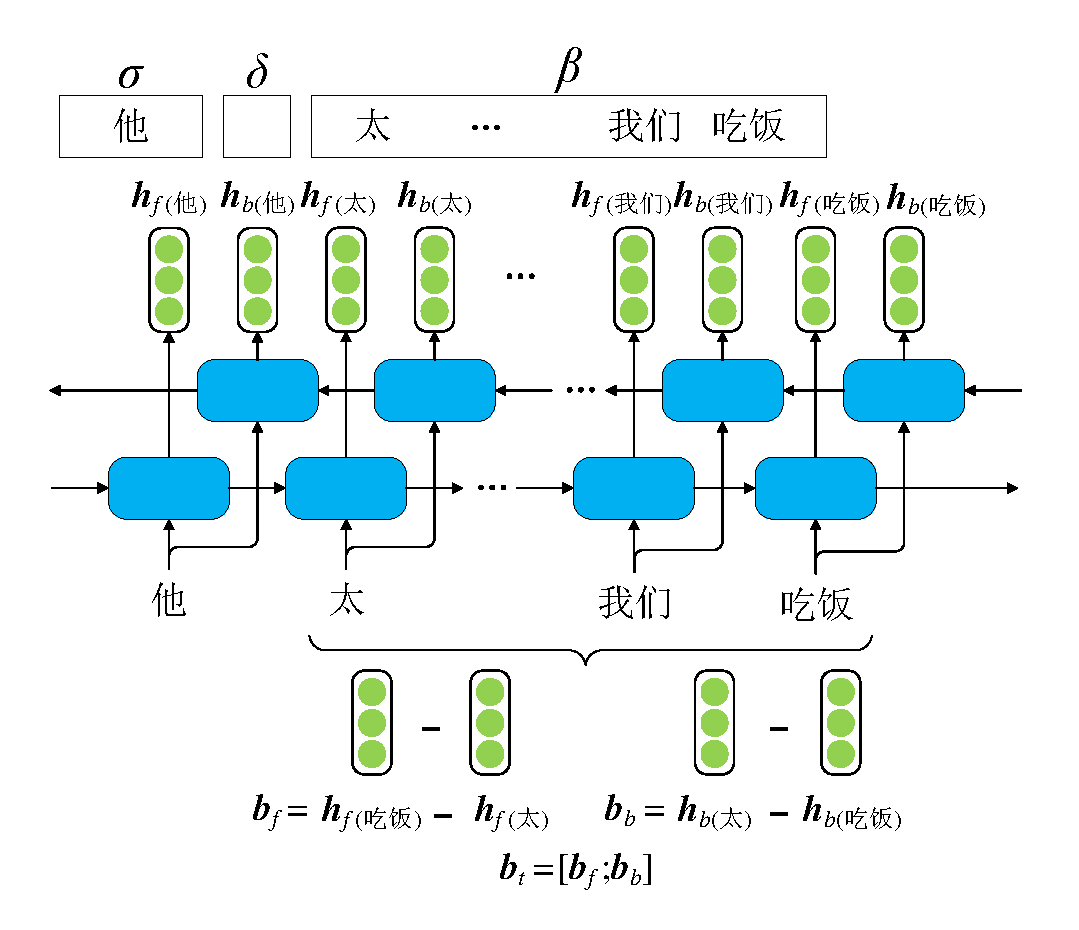
\includegraphics[width=0.7\textwidth]{figures/bs.pdf}
	\bicaption[fig:bs]{}{Bi-LSTM Subtraction模块结构图}{Fig.$\!$}{Model structure of Bi-LSTM Subtraction}
\end{figure}

图\ref{fig:bs}中给出了使用Bi-LSTM Subtraction模块计算列表的表示的例子。
首先使用“吃饭”的正向LSTM隐状态$\bm{h}_{f(\text{吃饭})}$减去“太”的正向LSTM隐状态$\bm{h}_{f(\text{太})}$,获得该段正向的表示向量,再用“太”的反向LSTM隐状态$\bm{h}_{b(\text{太})}$减去“吃饭”的反向LSTM隐状态$\bm{h}_{b(\text{吃饭})}$,获得该段反向的表示向量。
二者拼接起来作为此时列表的表示。

此外,原始的Stack-LSTM模型中使用基于依存的递归神经网络来计算转移过程中的子结构,在处理较深的子结构时,这种方法可能会遇到梯度消失问题。
为了解决该问题,本章在Tree-LSTM的基础上提出Incremental Tree-LSTM模块对这些子结构进行建模。
图\ref{fig:it}显示了本章提出的Incremental Tree-LSTM与基于依存的递归神经网络的区别。
递归神经网络通过递归地组合一个个父节点-子节点对来构建子图,而Tree-LSTM则能同时合并一个节点及其所有子节点。

由于基于转移的依存图分析的特点,本章中使用的Tree-LSTM与一般的Tree-LSTM有两点不同。
首先,该任务中需要建模的子结构不一定是树。
但由于需要处理的依存图不包括环,因此仍然能够使用LSTM。
更重要的是,与一般的Tree-LSTM能够同时获得一个节点的所有子节点不同,在基于转移的依存分析中,一个节点的子节点是逐个被找到的。
因此在Incremental Tree-LSTM中,需要不断利用Tree-LSTM更新父节点信息。
具体来说,对于一个词,每当找到它的一个新子节点,就要将其所有已经找到的子节点和其本身的表示输入Tree-LSTM中计算它的新表示。

\begin{figure}[hbtp]
	\centering
	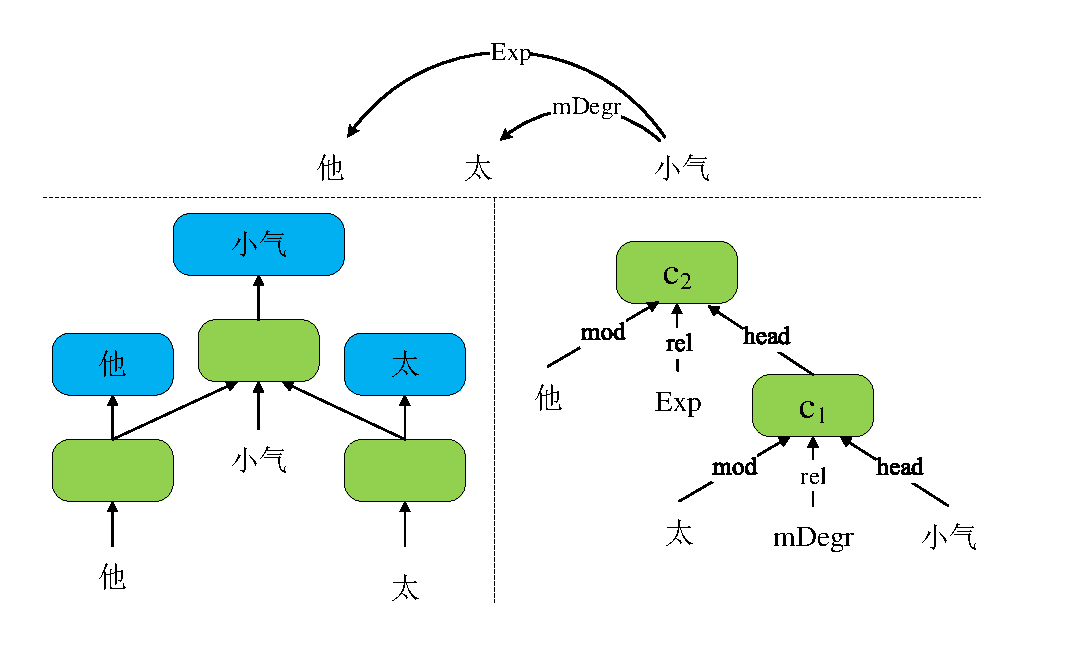
\includegraphics[width=0.9\textwidth]{figures/it.pdf}
	\bicaption[fig:it]{}{Incremental Tree-LSTM模块(左)与递归神经网络(右)对比图}{Fig.$\!$}{Comparison between Incremental Tree-LSTM and recursive neural network.}
\end{figure}

图\ref{fig:it}中给出了Incremental Tree-LSTM模块与递归神经网络在建模同一个子图时的对比图。
在转移过程中,“太”与“小气”之间的依存弧首先被生成,这时需要用Tree-LSTM合并二者的表示向量并将其作为“小气”的新表示。
在递归神经网络中,这一步的处理方法与Incremental Tree-LSTM模块基本相同,都是先合并“太”和“小气”的表示向量。
在第二步中,“小气”与其另一个子节点“他”之间的依存弧被生成,这时在Incremental Tree-LSTM模块中需要用Tree-LSTM合并“他”和“小气”的表示,以及之前已经找到的“小气”的子节点“太”的表示,将这三者表示合并之后作为父节点“小气”的新表示。
而在递归神经网络中,这一步则只需要合并“他”的表示向量之前已经生成的“太”和“小气”合并后的表示向量。
另外,值得注意的是,在Incremental Tree-LSTM模块中没有建模依存弧上的依存关系类别,而在递归神经网络中则建模了这一信息。
本章针对该问题使用原始Stack-LSTM模型进行了初步试验,发现从递归神经网络中删除依存关系类别信息并不会对最终结果产生太明显的影响。

\begin{figure}[hbtp]
	\centering
	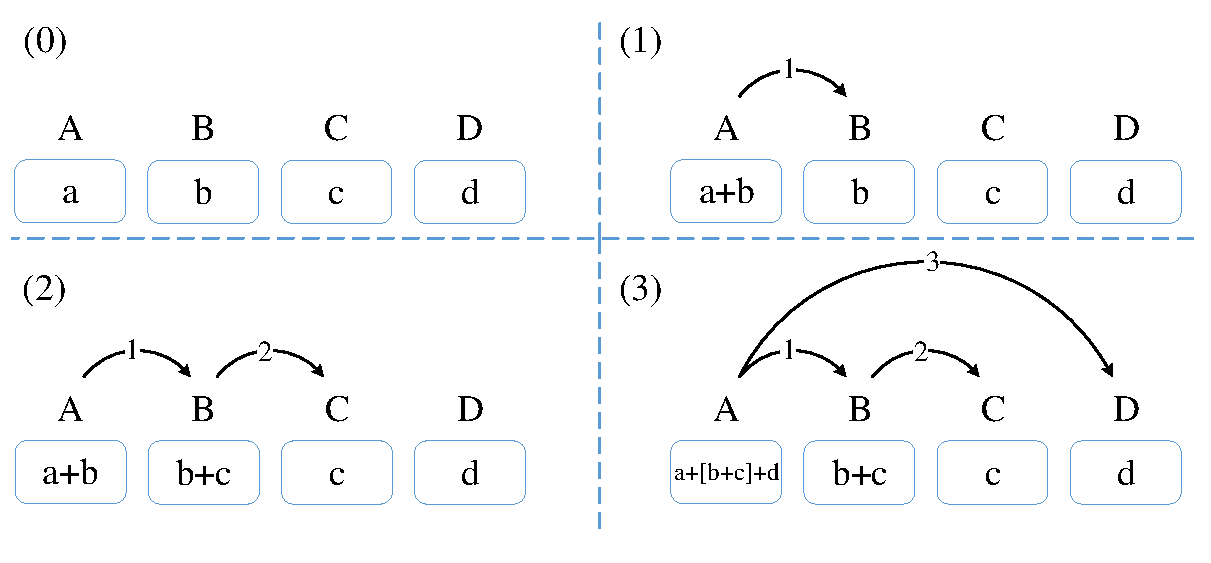
\includegraphics[width=0.9\textwidth]{figures/it-example.pdf}
	\bicaption[fig:it-example]{}{Incremental Tree-LSTM模块更新示例}{Fig.$\!$}{Example of updating in Incremental Tree-LSTM module.}
\end{figure}

为了进一步说明Incremental Tree-LSTM模块中根据当前生成的依存弧逐步更新Tree-LSTM状态的方式,图\ref{fig:it-example}给出了一个基于转移的依存分析中逐步生成的子图在Incremental Tree-LSTM模块中的更新过程的示例。
其中大写字母A、B、C、D表示句子中的词,小写字母a、b、c、d表示这些词对应的原始表示向量,而依存弧上的数字序号表示其生成的顺序。
该图中显示了以下4个状态:

1.初始状态下四个词之间还没有弧生成,这是他们的表示向量就是LSTM的隐层状态。

2.第一条由A指向B的依存弧生成后,A和B的表示向量a和b经过Tree-LSTM组合后代替A原来的表示向量。

3.第二条由B指向C的依存弧生成后,B和C的表示向量b和c经过Tree-LSTM组合后代替B原来的表示向量。

4.第三条由A指向D的依存弧生成后,A的原始表示向量a、B此时的表示向量b+c和D的表示向量d经过Tree-LSTM的组合后代替A原来的表示向量。

需要指出的是,在递归神经网络中,在第4步由A指向D的依存弧生成后,其只会直接将D的表示向量和A当时的表示向量(a+b)进行组合。
这样就遗漏了在前面的步骤中找到的B的子节点C的信息。
而在本章提出的Incremental Tree-LSTM模块中,这类信息则不会被遗漏。

\section{实验与分析}[Experiments and Analysis]

\subsection{实验设置}[Experimental Settings]

本章在中文和英文的语义依存图分析语料库上分别测试了BS-IT语义依存图分析模型的性能。
其中中文的语义依存图分析语料库来自SemEval-2016 Task 9\cite{che-etal-2016-semeval},是哈尔滨工业大学社会计算与信息检索研究中心和北京语言大学合作标注的中文语义依存图数据,其中按照句子来源分为两个子集,分别是新闻集(NEWS)和小学课本集(TEXT),前者句子较长、较复杂,后者句子较短、较简单。
而英文的语义依存图分析语料库来自SemEval-2015 Task 18\cite{oepen-etal-2015-semeval}英文广义语义依存图数据集。
该数据集一共有三种标注规范(DM、PAS和PSD),每种规范都有两部分测试数据集,即同领域(IN-DOMAIN)与异领域(OUT-OF-DOMAIN)测试数据。
中英文数据集的相关信息见表\ref{tbl:sdp-statistics}。
值得注意的是,由于DM、PAS和PSD是在相同的语料上按照不同的标注规范标注的,它们的各个集合的句子数是相同的,只有标签数量不同。

\begin{table}[htbp]
    \bicaption[tbl:sdp-statistics]{}{语义依存图语料库信息}{Table$\!$}{Statistics of Chinese semantic dependency graph dataset.}
    \vspace{0.5em}\centering\wuhao
    \begin{tabular}{ccccccc}
        \toprule[1.5pt]
        数据集 & 标签数 & 训练集 & 开发集 & 同领域测试集 & 异领域测试集 & 平均句子长度 \\
        \midrule[1pt]
        TEXT & 157 & 10,754 & 1,535 & 3,073 & 0     & 11.89 \\
        NEWS & 157 & 8,301  & 534   & 1,233 & 0     & 29.79 \\
        DM   & 61  & 33,964 & 1,692 & 1,410 & 1,849 & 22.26 \\
        PAS  & 43  & 33,964 & 1,692 & 1,410 & 1,849 & 22.26 \\
        PSD  & 92  & 33,964 & 1,692 & 1,410 & 1,849 & 22.26 \\
        \bottomrule[1.5pt]
    \end{tabular}
\end{table}

实验中使用的评测指标包括不计算弧标签的F值(UF)、计算弧标签的F值(LF)、有多父节点的词中不计算弧标签的F值(NUF)和有多父节点的词中计算弧标签的F值(NLF)。
其中值得注意的是NLF值,该指标只统计与有多个父节点的词相连的弧的计算标签的F值,也就是将目光集中在语义依存图分析中最难以解决的弧上,因此更能反映模型解决该问题的能力。

\subsection{实验结果}[Results]

\begin{table}[htpb]
    \bicaption[tbl:result-semeval16]{}{中文语义依存图数据集上的实验结果}{Table$\!$}{Results on Chinese semantic dependency graph dataset.}
    \vspace{0.5em}\centering\wuhao
	\begin{tabular}{lcccccccc}
		\toprule[1.5pt]
		\multirow{2}{*}{ 系统}&\multicolumn{4}{c}{NEWS}&\multicolumn{4}{c}{TEXT}\\
		%\cline{2-9}
		\cmidrule(r){2-5} \cmidrule(r){6-9}
		& LF& UF& NLF& NUF& LF& UF& NLF& NUF\\
		\midrule[1pt]
		IHS-RD-Belarus&59.06&77.64&40.84&60.20&68.59&82.41&50.57&64.58\\
		OCLSP (lbpg)&57.22&74.93&45.57&58.03&65.54&79.39&51.75&63.21\\
		OCLSP (lbpgs)&57.81&75.54&41.56&54.34&66.21&79.85&47.79&55.51\\
		OCLSP (lbpg75)&57.78&75.40&48.89&58.28&66.38&79.91&57.51&63.87\\
		OSU\_CHGCG&55.69&73.72&49.23&60.71&65.17&78.83&54.70&65.71\\
		Two-Stage & 62.29&80.56&39.93&64.29&71.94&85.24&50.67&69.97 \\ 
		Stack-LSTM &62.23&80.42&49.18&63.90&71.51&84.95&59.70&71.63\\
		BS-IT &\bf63.30&\bf81.14&\bf51.16&\bf66.92&\bf72.92&\bf85.71&\bf61.91&\bf72.74\\
		\bottomrule[1.5pt]
	\end{tabular}
\end{table}

表\ref{tbl:result-semeval16}中列出了中文语义依存图数据集上的实验结果。
下面分别介绍表中所列的各个基线模型:
\begin{itemize}
    \item IHS-RD-Belarus\cite{artsymenia-etal-2016-ihs}:该方法由Artsymenia等人于2016年提出,其中使用了包括在线重排序(online reordering)的基于转移的依存分析方法,并用预处理和后处理解决一些图结构的分析问题。
    \item OCLSP\cite{jin-etal-2016-oclsp}:该方法由Jin等人于2016年提出,其中使用了LSTM获取句中每个词的上下文相关表示,然后用这些表示向量计算句子中任意两个词之间存在弧的可能(lbpg)。
    由于其初始方法无法保证生成依存图,他们又使用了Chu-Liu-Edmond算法\cite{chu-liu-1965-shortest}进行解码(lbpgs)。
    另外他们还尝试了使用更高的阈值控制多父节点词出现的概率(lbpgs75)。
    
    \item OSU\_CHGCG\cite{duan-etal-2016-osu}:该方法由Duan等人于2016年提出,其中首先使用由中文广义范畴语法(Generalized Categorial Grammar,简称GCG)数据训练的分析器生成依存图结构,然后使用逻辑回归分类器为每条依存弧预测具体的语义关系。
    \item Two-Stage:该模型是参考Ding等人\cite{ding-etal-2014-dependency}于2014年提出的方法重新实现的基线模型。其中首先用传统依存树分析器预测出依存树结构,然后用一个支持向量机(Support Vector Machine,简称SVM)作为分类器从一个由规则产生的候选弧集合中选出一些弧加入其中组合成语义依存图。
    \item Stack-LSTM:该模型是在本章提出的基于转移的语义依存图分析系统中直接使用原始Stack-LSTM的基线模型。
\end{itemize}

表\ref{tbl:result-semeval16}中前5行是参加SemEval-2016 Task 9评测的系统的结果。
Two-Stage模型是本章重新实现的基线模型。
而Stack-LSTM模型可以认为是本章提出的BS-IT模型去掉Bi-LSTM Subtraction和Incremental Tree-LSTM两个模块后的结果。
BS-IT表示本章中提出的模型。
从实验结果中首先可以发现,本章重新实现的两个基线模型Two-Stage和Stack-LSTM都取得了显著高于此前模型的效果。
其中Two-Stage模型在整体的评价指标UF和LF上性能更高,而Stack-LSTM则在只考虑多父节点词的评价指标NUF和NLF上有更好表现。
其次,本章提出的BS-IT模型在所有评价指标上都显著超过了上述所有基线模型,尤其在对图结构评价至关重要的NLF值上提升明显。

\begin{table}[htpb]
    \bicaption[tbl:result-semeval15]{}{英文语义依存图数据集上的实验结果}{Table$\!$}{Results on English semantic dependency graph dataset.}
    \vspace{0.5em}\centering\wuhao
	\begin{tabular}{lcccc}
		\toprule[1.5pt]
		系统& DM & PAS & PSD & 宏平均\\
		\midrule[1pt]
		\multicolumn{5}{c}{IN-DOMAIN}\\
		\hline
		Du 15 (ensemble) &89.1&91.3&75.7&85.4\\
		Almeida 15 (single) &88.2&90.9&76.4&85.2\\
		Peng 17 (single) &89.4&\bf 92.2&77.6&86.4\\
		BS-IT (single) &89.3&91.4&76.1&85.6\\
		BS-IT (ensemble) &\bf 90.3& 91.7&\bf 78.6&\bf 86.9\\
		\hline
		\multicolumn{5}{c}{OUT-OF-DOMAIN}\\
		\hline
		Du 15 (ensemble) &81.8&87.2&73.3&80.8\\
		Almeida 15 (single) &81.8&86.9&74.8&81.2\\
		Peng 17 (single) &84.5&\bf 88.3&75.3&82.7\\
		BS-IT (single) &83.2&87.2&73.2&81.2\\
		BS-IT (ensemble) &\bf 84.9&87.6&\bf 75.9&\bf 82.8\\
		\bottomrule[1.5pt]
	\end{tabular}
\end{table}

表\ref{tbl:result-semeval15}中列出了英文语义依存图数据集上的实验结果,其中所列均为LF值,single表示单模型方法,ensemble表示多模型融合方法。
下面分别介绍表中所列的各个基线模型:
\begin{itemize}
    \item Du 15 \cite{du-etal-2015-peking} :该模型由Du等人于2015年提出,其中利用了多个不同的基于转移和基于图的模型同时预测并对最终结果进行投票。
    因此该模型是一个融合模型。
    \item Almeida 15 \cite{almeida-martins-2015-lisbon}:该模型由Almeida等人于2015年提出,其中使用了基于图的依存分析方法,使用了依存图结构中独有的二阶特征,并利用AD$^3$算法\cite{martins-etal-2011-dual}进行解码。
    \item Peng 17 \cite{peng-etal-2017-deep}:该方法由Peng等人于2017年提出,他们使用一个基于图的方法,同时利用英文语义依存图数据库中的三种标注体系进行多任务学习,取得了该数据集上当时最好结果。由于本章中并没有使用多任务学习方法,这里列出的是他们没有使用多任务学习的基础模型结果。
\end{itemize}

表\ref{tbl:result-semeval15}中BS-IT表示本章提出的系统的结果。
由于基线模型中有使用多模型融合的方法,表中也列出了将BS-IT方法与模型融合方法简单结合的结果。
具体实现方法是在训练时使用不同随机初始化种子训练多个模型。
在预测时,用这些模型算出的分数之和来选择接下来的转移动作。
实验证明该方法有效提高了系统性能,从而使本章提出的BS-IT模型达在英文语义依存图数据集三个标注体系的平均性能上超过了此前最好的模型。

\begin{table}[htpb]
	\bicaption[tbl:chapter2-ablation]{}{BS-IT模型各模块性能实验}{Table$\!$}{Effect of different modules of BS-IT model.}
    \vspace{0.5em}\centering\wuhao
	\begin{tabular}{clcccc}
		\toprule[1.5pt]
		Corpus& System & LF & UF & NLF & NUF\\
		\midrule[1pt]
		\multirow{4}{*}{NEWS}
		&Stack-LSTM&62.23&80.42&49.18&63.90\\
		&+BS &62.59&80.61&49.83&65.80\\
		&+IT &62.62&80.50&49.25&65.13\\
		&+BS\&IT &\bf63.30&\bf81.14&\bf51.16&\bf66.92\\
		\hline
		\multirow{4}{*}{TEXT}
		&Stack-LSTM&71.51&84.95&59.70&71.63\\
		&+BS &72.29&85.41&59.98&71.68\\
		&+IT &72.20&85.33&60.61&71.58\\
		&+BS\&IT &\bf72.92&\bf85.71&\bf61.91&\bf72.74\\
		\bottomrule[1.5pt]
	\end{tabular}
\end{table}

为了进一步证明BS-IT模型中的两个模块:Bi-LSTM Subtraction(BS)和Incremental Tree-LSTM(IT)的有效性,本章在中文语义依存图数据集上对它们进行了测试,结果如表\ref{tbl:chapter2-ablation}所示。
具体来说,该表中首先列出了只使用原始版本Stack-LSTM(即两个模块都不使用)的结果,然后分别列出了只使用其中之一的结果,最后列出了两个模块同时使用的结果。
从结果中可以发现,首先两个模块单独使用的效果都要优于原始版本的Stack-LSTM,即两个模块都能为Stack-LSTM模块带来性能上的提升。
其次,当同时使用两个模块时,模型取得了最好结果,这进一步说明了本章提出的Bi-LSTM Subtraction模块和Incremental Tree-LSTM模块的有效性。

\section{本章小结}[Conclusions]

本章针对语义依存图分析中的多父节点词问题设计了一套用于生成依存图的转移系统。
该系统无需预处理和后处理,能够自动根据输入句子生成完整的语义依存图。
此外,为了更高效、准确地获取转移系统中转移状态的表示,从而训练转移动作分类器预测下一步要执行的转移动作,本章在Stack-LSTM的基础上提出了Bi-LSTM Subtraction模块和Incremental Tree-LSTM模块,分别用于对转移系统中十分重要的列表和已生成的子图建模。
本文提出的语义依存图分析器完全摆脱了传统方法中需要专家知识的特征工程,实现了对依存图高效、自动地分析。
中文和英文的语义依存图数据集上的实验结果表明,本章提出的BS-IT模型与此前方法相比取得了显著的性能提升。

% Local Variables:
% TeX-master: "../thesis"
% TeX-engine: xetex
% End:
% !Mode:: "TeX:UTF-8"

\chapter[非规范文本语义依存图分析]{非规范文本语义依存图分析}[Semantic Dependency Graph Parsing on Informal Texts]

\section{引言}[Introduction]
\label{sec:chapter3-intro}

神经网络在自然语言处理领域的应用,不仅解决了传统的基于特征工程的统计学习模型中对专家知识的依赖,更有效提升了该领域各个任务上模型的性能\cite{chen-manning-2014-fast,chiu-nichols-2016-named,ma-hovy-2016-end,zhou-etal-2016-text,chopra-etal-2016-abstractive}。
随着2018年BERT模型的提出,以其为代表的预训练模型为自然语言处理领域带来了新一波的显著性能提升\cite{peters-etal-2018-deep,devlin-etal-2018-bert,yang-etal-2019-xlnet,clark-etal-2020-electra}。
然而,尽管在自然语言处理领域中的很多数据集上,神经网络模型已经取得了接近甚至超过人类的效果,但近期的研究表明,现有的神经网络模型鲁棒性很弱。
与其在规范文本组成的数据集上取得的成功相对应的是其在非规范文本上性能的大幅下降\cite{alzantot-etal-2018-generating, ren-etal-2019-generating, cheng-etal-2019-robust,michel-etal-2019-evaluation, jin-etal-2020-isbert}。

对神经网络模型的鲁棒性进行研究的一般方式是对抗样本攻击(adversarial attack),即设计算法针对特定的目标模型(target model或victim model)生成使其产生误判的非规范文本。
这种文本被称为对抗样本(adversarial example)。
目前自然语言处理领域的鲁棒性研究工作一般选择情感分类、文本蕴涵等文本分类任务作为目标任务。
针对这些任务的特点,高质量的对抗样本需要满足两个条件:(1)在语义上与原始文本相同;(2)对原始文本的修改难以被察觉。
其中第一点的作用是保证在有标注数据上,修改后的对抗样本的类别不会因修改而改变,这样才能利用原始本文上的标注信息对攻击算法的性能进行评价。
而第二点从另一个角度来说,就是要保持对抗样本的流畅性,使得人类不会因文本的修改而对其类别产生误判。
因为使人类也产生误判的对抗样本对于模型的鲁棒性研究来说毫无作用,其可能就是完全无意义的词语组合。

尽管目前已有不少研究者针对上述以分类任务上神经网络模型的鲁棒性开展研究,但很少有人研究句法依存分析和语义依存图分析等结构化预测任务上的神经网络模型鲁棒性。
虽然这类任务无法直接应用到日常生活中,但其预测结果往往被用于帮助其他能直接应用的任务。
而一旦其性能因为非规范文本而显著下降,错误级联效应会导致使用其输出的其他任务模型性能也受到影响。

此前虽然有少量针对句法依存分析模型鲁棒性的研究工作,但其往往只注重攻击算法本身,而采用了简单的候选词生成方法,从而影响了生成的对抗样本的质量。
针对这一问题,本章首先设计了一套针对基于神经网络的依存分析模型的攻击框架,使用了多种候选词生成方法生成大量候选词,接着使用多种过滤方法将其中不合适的过滤掉,从而保证了候选词的质量和数量,最终实现了高质量对抗样本的生成。
接着,本章借助该对抗样本攻击框架对现存的多种依存分析模型和词向量的组合进行了攻击,并设计了多项实验研究基于神经网络的依存分析模型的鲁棒性。
最后,依据在分析实验中的发现,本章提出两种提升现有基于神经网络的依存分析模型鲁棒性的方法,分别是对抗样本训练(adversarial training)和模型融合。

为了验证上述对抗样本攻击框架的有效性,本章分别在中文语义依存图分析任务和英文句法分析任务上进行了实验,并组织了针对对抗样本质量的人工评测。
结果表明上述方法有效提升了生成的对抗样本的质量,而对抗样本训练和模型融合都能有效提高现有的基于神经网络的依存分析模型的鲁棒性。

\section{背景与相关工作}[Related Work]

与重视语义的分类任务不同,在依存分析等结构化预测任务上,高质量的对抗样本需要满足两个条件:(1)语义或句法结构与原始文本相同;(2)文本流畅性。
其中第二点与分类任务中的条件相同,也是为了保证对抗样本不使人类产生误判。
而第一点则是为了保证原始文本上的人工标注信息在对抗样本上依然有效,这与分类任务中第一个条件有类似之处,但对于结构化预测任务更为严格。
这是因为首先结构化预测任务上的标注信息不仅只有一个标签,而是一个复杂的结构。
其次,相比于分类任务,结构化预测任务的标注更难以获取。
要使用正确的标注信息对攻击算法进行评价,往往只能保证修改后的文本上的结构不变。
正如第\ref{sec:chapter3-intro}节所介绍,目前虽然有少量针对句法依存分析模型鲁棒性的研究工作,但其往往忽略了对抗样本的质量。
本节将重点介绍与本章研究内容密切相关的针对依存分析模型鲁棒性进行研究的工作。

Zheng等人\cite{zheng-etal-2020-evaluating}于2020年在英文上首次开展了针对基于神经网络的句法依存分析模型的鲁棒性研究。
他们使用BERT模型基于上下文预测每个词的候选词,然后选择使目标模型性能下降最大的候选词替换原始文本中的词,从而实现对句法依存分析器的攻击。
具体来说,本文第\ref{sec:chapter1-informal}节已经介绍了BERT使用的遮盖语言模型训练目标,即通过将目标词遮盖然后用其上下文预测该词。
而该方法依次将目标句子中的每个词用BERT模型中特殊的遮盖符号进行替换,然后用BERT模型对该词进行预测,从而获取BERT模型词表中所有词在文本中该位置出现的概率。
然后再对这些词按照出现概率进行排序,选取其中前$N$个作为候选词。
需要特别说明的是,由于英文BERT模型使用的是词片段(word piece)向量而非词向量,其词表中很多都是不完整的词片段而非整词。
而不完整的词片段显然是无法替代原始句子中完整的词的,因此该方法只选择出现概率高的候选词中的整词作为候选词。
显然这种方法严重限制了候选词的多样性,而且由于英文中大部分复杂的词在BERT中都会被切割成词片段,这种方法无法生成这些复杂的词。

Han等人\cite{han-etal-2020-adversarial}于2020年在英文上开展了针对结构化预测任务上的神经网络模型的鲁棒性研究,并在句法依存分析任务上进行了实验。
他们提出一个序列到序列(sequence-to-sequence)模型,根据输入的原始文本生成对抗样本。
由于该模型无法保证生成的对抗样本与原始文本长度相同或具有相同的结构,该方法使用了两个额外的依存分析器的预测结果作为参考。
这两个额外的依存分析器与目标依存分析器要求是两两不同的依存分析模型,这样才能保证其预测结果与受攻击的目标分析器不同,且两个参考依存分析器之间才能互相验证。
该方法对于目标分析器和参考分析器的类别有较严格的要求,而且尽管其通过限制分析器类别提升了作为参考的预测结果的准确性,该方法仍然无法保证预测结果是完全正确的。
在这种情况下,使用预测的结果作为对抗样本正确标注对攻击方法进行评估也难以保证其准确率。

总的来说,此前的针对基于神经网络的依存分析模型的鲁棒性研究集中在英文的句法依存分析任务上,且往往忽略了生成的对抗样本质量。
而在对抗样本攻击中,对抗样本的质量是十分重要的,低质量的对抗样本很可能使人类也产生误判,从而对于模型鲁棒性的研究没有贡献。
另外,在对模型鲁棒性研究的基础上,如何提升依存分析模型的鲁棒性,也是亟待解决的问题。
因此,本章首先设计了针对依存分析模型生成高质量对抗样本的攻击框架,然后利用该框架对现有的依存分析模型鲁棒性进行研究,并在此基础上提出了提升其鲁棒性的方法。

\section{针对依存分析器的对抗样本攻击框架}[Adversarial Attacking Framework against Dependency Parsers]

研究表明,在深度神经网络输入中加入微小扰动信息,能够使其产生误判。
这种使神经网络产生误判的攻击称为对抗样本攻击,其中使用的输入样本称为对抗样本。
尽管基于深度神经网络的模型在自然语言处理领域的很多任务上都取得了很好的成果,但对抗样本攻击揭示了这类模型脆弱的一面。
为了提高现有依存分析器的鲁棒性,使其适用于现实复杂场景,我们首先设计对抗样本攻击算法,针对现有各类依存分析器生成对抗样本,并对生成的样本进行分析,在此基础上提出了增强分析器鲁棒性的方法。

根据攻击者对目标系统的了解程度,对抗样本攻击可以大致分为白盒攻击和黑盒攻击两类。
在白盒攻击情景下,攻击者能获取目标系统的所有信息,包括模型结构,参数及权重值等。
而在黑盒攻击情景下,攻击者仅能用对目标系统查询的方式,通过输入观察输出结果。
这里我们选择更贴近现实情况的黑盒攻击情景,设计了一个黑盒攻击框架,针对现有依存分析器生成对抗样本。
图~\ref{fig:adv-example}展示了一个我们的攻击框架生成的对抗样本,其中上半部分为原始文本及正确的依存句法预测结果,下半部分为我们生成的对抗样本及目标分析器预测结果(红色部分表示预测错误的依存弧和标签)。
在该实例中,我们的攻击框架只修改了一个词(将highway改为superhighway),就使得目标分析器产生了5个错误。

\begin{figure}[htbp]
	\centering
	\begin{dependency}[theme = simple,label style={font=\bfseries}]
		\begin{deptext}[column sep=0.45em]
			A\& bus\& is\& the\& data\& \textcolor{green}{highway}\& within\& a\& computer \\ %\& . \\
			A\& bus\& is\& the\& data\& \textcolor{red}{\textit{\textbf{superhighway}}}\& within\& a\& computer \\%\& . \\
		\end{deptext}
		\deproot{6}{root}
		\depedge{2}{1}{det}
		\depedge{6}{2}{nsubj}
		\depedge{6}{3}{cop}
		\depedge{6}{4}{det}
		\depedge{6}{5}{nn}
		\depedge{6}{7}{prep}
		\depedge{9}{8}{det}
		\depedge{7}{9}{pobj}
		%\depedge{6}{10}{punct}
		
		\deproot[edge below, dashed, edge style={red}, label style={below, font=\bfseries, text=red}]{5}{\textit{root}}
		\depedge[edge below, label style={below}]{2}{1}{det}
		\depedge[edge below, dashed, edge style={red}, label style={below, font=\bfseries, text=red}]{5}{2}{nsubj}
		\depedge[edge below, dashed, edge style={red}, label style={below, font=\bfseries, text=red}]{5}{3}{cop}
		\depedge[edge below, dashed, edge style={red}, label style={below, font=\bfseries, text=red}]{5}{4}{det}
		\depedge[edge below, dashed, edge style={red}, label style={below, font=\bfseries, text=red}]{5}{6}{\textit{partmod}}
		\depedge[edge below, label style={below}]{6}{7}{prep}
		\depedge[edge below, label style={below}]{9}{8}{det}
		\depedge[edge below, label style={below}]{7}{9}{pobj}
		%\depedge[edge below, dashed, edge style={red}, label style={below, font=\bfseries, text=red}]{5}{10}{\textit{punct}}
	\end{dependency}
	\caption{对抗样本实例}
	\label{fig:adv-example}
\end{figure}

下面我们首先给出针对依存分析器攻击的形式化定义。
给定包括所有可能输入句子$\bm{x}$的输入文本空间$\mathcal{X}$和包括$\bm{x}$所有可能依存树的输出空间$\mathcal{Y}$。
一个依存分析器$F: \mathcal{X} \rightarrow \mathcal{Y}$的目标是学习一个从输入句子$\bm{x}$到其对应依存树$\bm{y}$的映射,记为$F(\bm{x}) = \bm{y}$。
句子$\bm{x}$中的第$i$个词记为$x_i$,用$(i,j,r) \in \bm{y}$表示依存树$\bm{y}$中存在一条由$x_i$指向$x_j$,标签为$r$的弧。

给定一个句子$\bm{x}$,我们通过对其进行微小的修改获得$\bm{x}^*$,当$\bm{x}^*$满足以下条件时,将其称为一个有效的对抗样本:
$$F(\bm{x}^*) \neq \bm{y}, \sigma(\bm{x}^*, \bm{x})\le \epsilon, $$
其中$\sigma$为样本变化约束函数,$\epsilon$为原始句子$\bm{x}$与对抗样本$\bm{x}^*$间可允许的最大差别。

我们提出的针对依存分析器的黑盒攻击框架如算法~\ref{algo:attack}所示,由词重要性排序(1-4行)、候选词生成(第7行)和替换词搜索(8-21行)三部分组成。
其基本思路是对句中每个词生成若干能保证句法结构不变和语法正确的候选词,按照句中词的重要性由高到低搜索并替换能使目标分析器预测准确率下降的候选词。


\begin{algorithm}[!h]
    \wuhao
	%\begin{flushleft}
	%	\textbf{Input:} 原始样本 $\bm{x}^{(0)}=\{x_1,x_2,\dots,x_N\}$, 最大允许修改百分比 $\gamma$ \\
	%	\textbf{Output:} 对抗样本 $\bm{x}^{(i)}$
	%\end{flushleft}
	\LinesNumbered %要求显示行号
    \KwIn{原始样本 $\bm{x}^{(0)}=\{x_1,x_2,\dots,x_N\}$, 最大允许修改百分比 $\gamma$}%输入参数
    \KwOut{对抗样本 $\bm{x}^{(i)}$}%输出
		\For{$i=1$ to $N$}
		{
		    用公式~\ref{eq:word-importance}计算词重要性$I(\bm{x}^{(0)},x_i)$\;
		}
		建立一个由$x_i\in\bm{x}^{(0)}$组成的集合$W$,其中词按照重要性$I(\bm{x}^{(0)},x_i)$从高到低排序\;
		$t=0$\;
		\For{$W$中每个$x_j$}
		{
		    按照候选词生成步骤建立词$x_j$的候选词集合$\mathcal{C}_j$\;
		    初始化有效候选词集合$\mathcal{VC} \leftarrow \{\}$\;
		    \For{$\mathcal{C}_j$中每个候选词$c_k$}
		    {
		        用公式~\ref{eq:mis-inc}计算准确率改变量$S(\bm{x}^{(t)},c_k,j)$\;
		        \If{$S(\bm{x}^{(t)},c_k,j) > 0$}
		        {
		            将$c_k$加入集合$\mathcal{VC}$
		        }
		        %\algorithmicif\  $S(\bm{x}^{(t)},c_k,j) \le 0$\ \algorithmicthen\ continue\ \algorithmicendif\
		        %将$c_k$加入集合$\mathcal{VC}$\;
		    }
		}
		\If{$\mathcal{VC}$非空}
		{
		    $c^* = \argmaxl_{c \in \mathcal{VC}} S(\bm{x}^{(t)},c,j)$\;
    		$t = t + 1$\;
    		$\bm{x}^{(t)} \leftarrow \text{将} \bm{x}^{(t-1)} \text{中的} x_j  \text{替换为} c^*$\;
    		\If{$t \ge \gamma \cdot N $}
    		{
    		    \algorithmicreturn\ $\bm{x}^{(t)}$
    		}
    		%\algorithmicif\  $t \ge \gamma \cdot N $\ \algorithmicthen\   \algorithmicreturn\ $\bm{x}^{(t)}$\ \algorithmicendif\;
		}
		\eIf{$t > 0$}
		{
		    \algorithmicreturn\ $\bm{x}^{(t)}$
		}
		{
		    \algorithmicreturn\ None
		}
		%\algorithmicif\  $t > 0$\ \algorithmicthen \algorithmicreturn\ $\bm{x}^{(t)}$\ \algorithmicelse\ \algorithmicreturn\ None \algorithmicendif
	\AlgoBiCaption{针对依存分析器的黑盒攻击算法}{Black-box attack algorithm against dependency parsers.}
	\label{algo:attack}
	%\bicaption[algo:attack]{算法}{针对依存分析器的黑盒攻击算法}{Algo.$\!$}{Effect of different modules of BS-IT model.}
\end{algorithm}


\subsection{词重要性排序}[Word Importance Ranking]

在一个句子中,不同的词对于模型的预测结果会产生不同程度的影响,我们将这种影响的大小视为词的重要性,对句中词按重要性进行排序。
此前的方法通过将句中词逐个替换为未知标签并计算替换前后模型预测结果的改变获得词的重要性。\cite{li2016visualizing,ren2019generating}
针对依存分析任务,我们用替换前后无标记依存正确率(Unlabled Attachment Score,UAS)和带标记依存正确率(Labled Attachment Score,LAS)的改变量作为衡量词重要性的分数。
具体来说,句子$\bm{x}$中词$x_i$的重要性为:

\begin{equation}
	\label{eq:word-importance}
	I(\bm{x},x_i) = \lambda_{arc}\Delta_\text{UAS}(\bm{x},\hat{\bm{x}_i}) + (1-\lambda_{arc})\Delta_\text{LAS}(\bm{x},\hat{\bm{x}_i}),
\end{equation}
其中$\bm{x} = x_1x_2\dots x_i\dots x_N$为原始句子,$\hat{\bm{x}_i} = x_1x_2\dots \text{UNK}\dots x_N$为将词$x_i$替换为特殊未知词标签UNK的修改后句子。
$\Delta_\text{UAS}(\bm{x},\hat{\bm{x}_i}) = \text{UAS}(F(\bm{x})) - \text{UAS}(F(\hat{\bm{x}_i})) $和$\Delta_\text{LAS}(\bm{x},\hat{\bm{x}_i}) = \text{LAS}(F(\bm{x})) - \text{LAS}(F(\hat{\bm{x}_i}))$分别表示修改前后UAS和LAS的改变量。
$\lambda_{arc}$为用于调节依存弧和标签之间相对重要性的系数。在实验中我们将其设为0.5。


\subsection{候选词生成}[Generation of Substitute Candidates]
\label{sec:gen-cand}

候选词生成中我们针对句中每个目标词,生成若干候选词,为后续的替换做准备,这一步很大程度上影响到了攻击成功率和对抗样本的质量。
此前的工作尝试了包括基于语言模型的\cite{zheng2020evaluating}、基于词向量的\cite{alzantot2018generating}、基于同义词的\cite{ren2019generating}和基于义原(Sememe)的\cite{zang2020word}生成策略。
这些策略各自存在不同的问题,前两类生成的候选词质量无法保证,而后两类生成候选词的数量受到限制。
为了解决这些问题,我们首先同时用这四类策略生成候选词集合,之后使用四种过滤策略过滤掉不合适的候选词,从而同时保证了候选词的质量和数量。

我们首先用以下四种策略生成候选词:

\textbf{基于语言模型的方法} \ \ 我们使用预训练的语言模型(BERT),将目标词逐一遮盖(mask)并用其上下文重新预测该词,选取前$k$个作为候选词。

\textbf{基于词向量的方法} \ \ 我们使用Mrksic等人的词向量\cite{mrksic2016counter}的cosine相似度计算每个目标词的N个最近的词,将其作为候选词。

\textbf{基于近义词的方法} \ \ 我们使用WordNet\footnote{\url{https://wordnet.princeton.edu}}抽取每个目标词的所有近义词作为候选词。

\textbf{基于义原的方法} \ \ 义原在语言学中指最小的不可再分的语义单位。\cite{dong2006hownet} 对于每个候选词,我们根据HowNet中定义的义原,收集所有至少有一个义原与其重复的词作为其候选词。

在用上述方法获得若干候选词之后,我们依次使用以下四种过滤策略,将候选词集合中不合适的词过滤掉:

\textbf{词性过滤} \ \ 我们首先过滤掉候选词中与目标词词性不同的,这是为了确保替换后句法结构不变。

\textbf{语法检测过滤} \ \ 我们使用公开的语法检测工具\footnote{\url{https://pypi.org/project/language_tool}}过滤掉替换后会引入语法错误的候选词,从而进一步确保句法结构的不变性和语法的正确性。


\textbf{词向量相似度过滤} \ \ 我们使用词向量cosine相似度过滤掉与目标词相似度低于$\epsilon_w$的候选词。

\textbf{困惑度过滤} \ \ 对于每个候选词$c \in \mathcal{C}$,我们使用预训练的语言模型GPT-2计算原始句子$\bm{x}$和替换后句子$\bm{x}^c_{i}$的困惑度,定义困惑度增量为:
\begin{equation}
	\label{eq:ppl-inc}
	\Delta \text{ppl}(\bm{x},c,i)=\max(\text{ppl}(\bm{x}^c_{i})-\text{ppl}(\bm{x}), 0),
\end{equation}
其中$\bm{x}^c_{i}$为将原始文本$\bm{x}$的第$i$个词替换为$c$后的文本。
我们将$\Delta\text{ppl}(\bm{x},c,i) > \epsilon_p$的候选词过滤掉。


\subsection{替换词搜索}[Best Substitute Searching]

在这一步,我们用贪心搜索策略按照目标词重要性由高到底搜索其候选词,找到合适的替换词。
为了保持句子的句法结构不变,在搜索中我们不允许替换代词、冠词、连词、数字、感叹词、限定疑问词和标点符号。
此外,为了控制修改词的个数,在实验中我们设置了最大允许修改百分比$\gamma$(实验中设为15\%)。

具体来说,给定句子$\bm{x}$,我们按照目标词重要性从高到低对其进行排序,并按此顺序进行搜索。
对每个目标词$x_i$,我们用其候选词集合$\mathcal{C}$中的每个候选词$c$构建一个对抗样本$\bm{x}^c_{i} = x_1x_2\dots c\dots x_N$,并计算目标分析器分别以$\bm{x}$和$\bm{x}^c_{i}$为输入时的准确率差值:

\begin{equation}
	\begin{aligned}
		\label{eq:mis-inc}
		S(\bm{x},c,i) = & \lambda_{arc}\Delta_\text{UAS}(\bm{x},\bm{x}^c_{i}) + \\ 
		& (1-\lambda_{arc})\Delta_\text{LAS}(\bm{x},\bm{x}^c_{i}),
	\end{aligned}
\end{equation}
其中$\Delta_\text{UAS}(\bm{x},\bm{x}^c_{i}) = \text{UAS}(F(\bm{x})) - \text{UAS}(F(\bm{x}^c_{i})) $和$\Delta_\text{LAS}(\bm{x},\bm{x}^c_{i}) = \text{LAS}(F(\bm{x})) - \text{LAS}(F(\bm{x}^c_{i}))$分别为UAS和LAS的改变量。 
$\lambda_{arc}$是一个控制依存弧和标签相对重要性的系数,在实验中设为0.5。

如果没有一个候选词$c$使得$S(\bm{x},c,i) > 0$,换句话说,如果没有候选词能马上使准确率降低,则跳过这个目标词,开始搜索下一个目标词的候选词。
否则,我们就选择准确率该变量$S(\bm{x},c,i)$最大的候选词$c$,并用其替换$x_i$。
接着,如果该句子中已修改的词占比超过了$\gamma$,则停止搜索返回当前句子。
否则继续搜索下一个目标词的候选词。


\section{对抗样本攻击实验结果与分析}[Experiments and Analysis of Adversarial Attack]


\subsection{实验设置}[Experimental Settings]


\subsection{实验结果}[Results]

我们在依存句法分析领域应用最广的宾州树库(Penn Treebank,PTB)上测试了我们的攻击框架,并与此前工作进行了对比。
我们选择了依存分析任务中两个具有代表性的分析器Biaffine分析器\cite{dozat2017deep}和Stack-Pointer分析器\cite{ma2018stack}作为攻击目标,其中前者是基于图的分析器,后者是基于转移的分析器。
在目前广泛应用的深度神经网络模型中,输入词向量往往对模型性能产生至关重要的影响。
为了测试不同类型的词表示作为输入时目标分析器的鲁棒性,我们选择了以下四种有代表性的词表示:

\textbf{GloVe}\cite{pennington2014glove}是一个常用的固定上下文无关词向量。

\textbf{RoBERTa}\cite{liu2019roberta}是一个预训练语言模型,其训练目标为掩码语言模型(masked language modeling,MLM),目标是通过上下文预测被遮盖的词。 该模型生成的是上下文相关子词(sub-word)向量。

\textbf{ELECTRA}\cite{clark2020electra}是另一个预训练语言模型,其训练目标为替换词检测( replaced token detection),目标是预测被修改的输入文本中哪个词被修改过。
该模型生成的是上下文相关子词(sub-word)向量。

\textbf{ELMo}\cite{peters2018deep}是一个基于字母向量的预训练语言模型,其训练目标为双向语言模型。 

\begin{table}[h]
	\centering
	\small
	\renewcommand{\arraystretch}{1.2}
	\begin{tabular}{l|cccc}
		\hline
		\bf 模型& \bf 原始UAS & \bf 攻击后UAS & \bf 成功率\% & \bf 平均修改词数 \\
		\hline
		\bf Zheng et al. & 95.52 & 88.69 & 51 & 2.23 \\
		\textbf{Ours} & 95.45 & \bf 86.53 & \bf 52 & \bf 1.36 \\
		\hline
	\end{tabular}
	\caption{PTB-SD-3.3.0-COP测试集上的结果} 
	\label{tbl:attack-cop}
\end{table}

表~\ref{tbl:attack-cop}中列出了我们的模型(\textbf{Ours})与此前工作的对比。
由于Zheng等人对PTB的预处理与普遍使用的略有不同,我们为了与他们的结果进行对比,先用他们的处理方式生成了PTB-SD-3.3.0-COP数据集并在该数据集上与他们进行了对比。
实验结果表明我们的方法获得了更高的攻击成功率。
此外,我们的平均修改词数几乎只有他们的一半,这说明我们的攻击效率要显著高于他们。

为了进一步对比各攻击方法生成的对抗样本的质量,我们采用人工评价的方法,从句法结构不变性和语法正确性两方面对样本质量进行评价。
为了评价句法结构不变性,我们随机选择了100个句子和对应的对抗样本,让三位人类评价者判断修改后是否改变了句法结构。
结果显示其中87\%的句子句法结构都是不变的。而Zheng等人进行的相同人工评价结果显示他们的对抗样本中仅75\%的句子句法结构不变。
为了评价语法正确性,我们随机挑选了100个句子,将我们和他们模型生成的对抗样本同时提供给人类评价者,让其选择哪个样本更好的保证了语法正确性(允许选择二者语法正确性同样好)。
结果显示对于56\%的句子我们的对抗样本更好,对于19\%的句子他们的更好,剩余25\%二者同样好。

\begin{table}[htbp]
	\centering
	\small
	\renewcommand{\arraystretch}{1.2}
	\begin{tabular}{l|l||cc|cc|c|c}
		\hline
		\multirow{2}{*}{\bf 分析器}&\multirow{2}{*}{\bf 输入}& \multicolumn{2}{c|}{\bf 原始结果} & \multicolumn{2}{c|}{\bf 攻击后结果} & \multirow{2}{*}{\bf 成功率\%} & \multirow{2}{*}{\bf 平均修改词数} \\
		\cline{3-6}
		& & \bf UAS & \bf LAS & \bf UAS & \bf LAS & & \\
		\hline
		\multirow{4}{*}{\bf Biaffine} & \bf Glove &95.51 & 93.71 &87.79 &83.57 &61.4 &1.28 \\
		& \bf ELMo  &96.38 &94.60 &91.00 &87.40 &50.1 &0.95 \\
		& \bf ELECTRA &97.09 & 95.35 &90.63 &86.97 &55.8 &1.10 \\
		& \bf RoBERTa &96.83 & 95.15 &92.54 &89.26 &49.2 &0.89 \\
		\hline
		\hline
		\multirow{4}{*}{\bf Stack-Pointer} & \bf Glove &95.10 & 93.29 &87.71 &83.45 &59.3 &1.12 \\
		& \bf ELMo    &95.69 & 93.79 &89.93 &86.28 &49.3 &0.88 \\
		& \bf ELECTRA &96.90 & 95.16 &90.11 &86.39 &56.1 &1.08 \\
		& \bf RoBERTa &96.64 & 94.83 &92.39 &89.09 &48.8 &0.87 \\
		\hline
	\end{tabular}
	\caption{PTB-SD-3.3.0测试集上的结果} 
	\label{tbl:attack-main}
\end{table}

为了方便此后的工作进行对比,我们使用PTB普遍的预处理方式生成的PTB-SD-3.3.0数据集,并在该数据集上进行了大量实验,对比了两类分析器和四类词向量在我们的攻击框架下的性能,结果见表~\ref{tbl:attack-main}。
结果显示基于图的Biaffine分析器在输入向量相同的情况下普遍好于基于转移的Stack-Pointer分析器,而二者面对对抗样本攻击时鲁棒性差距不大。
在四种输入表示中,ELECTRA在原始文本作为输入时取得最好实验结果,RoBERTa次之,GloVe最差。
但在面对对抗样本攻击时,RoBERTa表现最好,ELMo也表现出了近似的鲁棒性,而ELECTRA则变现的很不好,其攻击成功率仅次于GloVe。
我们推测这可能是因为ELECTRA的训练目标是预测句中哪个词被修改过,而这种训练目标使得其将很多正确的替换词也视为错误,从而降低了它的鲁棒性。


\begin{table}[h]
	\centering
	\small
	\renewcommand{\arraystretch}{1.2}
	\begin{tabular}{l||cc|cc|c}
		\hline
		\multirow{2}{*}{\bf 词表}& \multicolumn{2}{c|}{\bf 原始结果} & \multicolumn{2}{c|}{\bf 攻击后结果} & \multirow{2}{*}{\bf 成功率\%} \\
		\cline{2-5}
		& \bf UAS & \bf LAS & \bf UAS & \bf LAS & \\
		\hline
		\bf Base &\multirow{3}{*}{95.51} & \multirow{3}{*}{93.71} &87.79 &83.57 &61.4 \\
		\bf Large  & & &88.39 &84.37 &58.7 \\
		\bf Base (T.) && &89.97 &86.67 &49.7 \\
		\hline
	\end{tabular}
	\caption{不同词表大小模型在PTB-SD-3.3.0测试集上的结果} 
	\label{tbl:oov-oot-result}
\end{table}

\begin{table}[h]
	\centering
	\small
	\renewcommand{\arraystretch}{1.2}
	\begin{tabular}{l||cc|cc}
		\hline
		\multirow{2}{*}{\bf 词表}& \multicolumn{2}{c|}{\bf 原始结果} & \multicolumn{2}{c}{\bf 攻击后结果}  \\
		\cline{2-5}
		& \bf OOV & \bf OOT & \bf OOV & \bf OOT \\
		\hline
		\bf Base &7 &39 &1192 &1207 \\
		\bf Large  &0 &34 &1 &995  \\
		\bf Base (T.) &3 &19 &0 &0 \\
		\hline
	\end{tabular}
	\caption{表~\ref{tbl:oov-oot-result}中未登录词和未在训练集出现词数}
	\label{tbl:oov-oot-num}
\end{table}

为了探究未登录(Out-of-Vocabulary,OOV)词和未在训练集出现(Out-of-Training,OOT)词对于对抗样本攻击的影响,我们用Biaffine分析器和GloVe向量进行了实验,在训练时使用不同大小的词表,实验结果见表~\ref{tbl:oov-oot-result}。
其中\textbf{Base}模型词表大小为39073,而\textbf{Large}模型词表大小为371025。
\textbf{Base (T.)}表示在对\textbf{Base}模型攻击时只允许从训练集中出现过的词中搜索替换词。
而相应的攻击前后未登录词和未在训练集出现词的数量见表~\ref{tbl:oov-oot-num}。
对比\textbf{Base}和\textbf{Large}模型被攻击前后的实验结果及未登录词数量统计,我们有理由认为对抗样本中出现的未登录词会引起模型预测错误。
而更大的词表能通过降低未登录词出现的可能性从而有效增强模型的鲁棒性。
此外,通过对比\textbf{Base}和\textbf{Base (T.)}的结果,我们可以认为未在训练集中出现过的词也会降低模型预测的准确率。

针对未在训练集中出现过的词,一个可能的解决方案是对抗学习,即使用对抗攻击算法对训练数据生成对抗样本,然后用原始训练数据和对抗样本混合训练分析器。
此前的工作\cite{zheng2020evaluating}已证明此方法的有效性。
然而在现实情况下我们很难在训练时就获知对抗攻击算法,而且使用这种对抗学习也有使得模型过拟合到对抗样本的风险。
因此我们基于上文实验的观察结果,提出几种不需要对抗攻击算法就能增强模型鲁棒性的方法。

\begin{itemize}
	\item \textbf{使用更大的词表(Large)} \ \ 更大的词表能够降低未登录词在对抗样本中出现的可能性,从而有效增强模型的鲁棒性。
	\item \textbf{未知词替换(UNK)} \ \ 在训练过程中将不常见的词替换为特殊的未知词表示UNK,在预测过程中如果出现未登录词,则用UNK代替,这样能确保即使遇到未登录词,模型也能对其表示有一个估计。
	\item \textbf{模型融合(ensemble)} \ \ 融合多个用不同随机初始化种子训练的模型能有效增加系统的稳定性,从而增强模型的鲁棒性。
\end{itemize}

\begin{table}[h]
	\centering
	\small
	\renewcommand{\arraystretch}{1.2}
	\begin{tabular}{l||cc|cc|c}
		\hline
		\multirow{2}{*}{\bf 强化策略}& \multicolumn{2}{c|}{\bf 原始结果} & \multicolumn{2}{c|}{\bf 攻击后结果} & \multirow{2}{*}{\bf 成功率\%} \\
		\cline{2-5}
		& \bf UAS & \bf LAS & \bf UAS & \bf LAS & \\
		\hline
		\bf Base &95.51 &93.71 &87.79 &83.57 &61.4 \\
		\bf Large &95.51 &93.71 &88.39 &84.37 &58.7 \\
		\bf Large+UNK &95.57 &93.77 &88.98 &85.15 &57.0 \\
		\bf Large+UNK+ensemble &95.62 &93.80 &89.49 &85.53 &55.8 \\
		\hline
	\end{tabular}
	\caption{PTB-SD-3.3.0测试集上的鲁棒性测试结果} 
	\label{tbl:attack-increase}
\end{table}

表~\ref{tbl:attack-increase}中列出了使用上述策略后模型面对对抗样本攻击的实验结果。
结果显示这三种策略都能有效提高模型鲁棒性,降低攻击成功率。
当这三者结合起来的时候效果最好。
由于我们在训练过程中没有使用任何对抗样本,这三种策略也没有使模型过拟合到某种特定攻击的风险。
这部分工作已投往AAAI 2021,后续计划将该攻击框架的目标扩展到语义依存图分析。


\section{依存分析模型的鲁棒性提升方法}[Robustness Increasing Approaches for Dependency Parsers]

\subsection{基于模型融合的鲁棒性提升方法}[Robustness Increasing Approach Based on Model Ensemble]

\subsection{基于对抗样本训练的鲁棒性提升方法}[Robustness Increasing Approach Based on Adversarial Training]


\section{实验与分析}[Experiments and Analysis]

\subsection{实验设置}[Experimental Settings]


\section{本章小结}[Conclusions]


% Local Variables:
% TeX-master: "../thesis"
% TeX-engine: xetex
% End:
% !Mode:: "TeX:UTF-8"

\chapter[跨语言语义依存图分析]{跨语言语义依存图分析}[Cross-Lingual Semantic Dependency Graph Parsing]

\section{引言}[Introduction]

\section{背景与相关工作}[Related Work]

\section{跨语言语义依存图数据库的构建}[Construction of Cross-Lingual Semantic Dependency Graph Dataset]

\subsection{跨语言语义依存图标注规范}[Annotation Guidelines for Cross-Lingual Semantic Dependency Graph]

\subsection{基于标签转换的自动标注转化方法}[Annotation Conversion Based on Label Switching]

\subsection{基于图神经网络的自动标注转化方法}[Annotation Conversion Using Graph Neural Networks]

\section{跨语言语义依存分析}[Cross-Lingual Semantic Dependency Graph Parsing]

\subsection{基于跨语言上下文相关词向量的零样本学习方法}[Zero-Shot Cross-Lingual Semantic Dependency Graph Parsing Based on Cross-Lingual Contextual Embeddings]

\subsection{基于数据增强的半监督方法}[Semi-Supervised Cross-Lingual Semantic Dependency Graph Parsing Based on Data Augmentation]

\section{实验与分析}[Experiments and Analysis]

\subsection{实验设置}[Experimental Settings]


\section{本章小结}[Conclusions]


% Local Variables:
% TeX-master: "../thesis"
% TeX-engine: xetex
% End:
% !Mode:: "TeX:UTF-8"

\chapter[基于字级别依存关系的语义依存图应用]{基于字级别依存关系的语义依存图应用}[Semantic Dependency Graph Application Based on Character-Level Dependency]

\section{引言}[Introduction]
\label{sec:chapter5-intro}

以句法依存树为代表的结构化信息,在传统的神经网络模型中被广泛应用于句子信息的获取。
例如,Socher等人\cite{socher-etal-2011-parsing}在2011年提出了递归神经网络,利用句法结构对文本进行编码。
随后在2015年,Tai等人在此基础上提出了Tree-LSTM,用于解决递归神经网络训练过程中的梯度消失和梯度爆炸问题。
随后一系列图神经网络\cite{kipf-welling-2017-semi, velickovic-etal-2018-gat}的提出,为自然语言处理领域的研究者提供了更多将句法等结构化信息融入神经网络模型中的选择。


自2018年以来,随着以BERT为代表的预训练模型在自然语言处理领域逐渐占据主流地位,其强大的表示和抽象能力使得结构化信息的作用开始受到质疑。
研究者开始设计方法对BERT中是否已经隐含句法等结构信息进行探测。
其中,Hewitt等人\cite{hewitt-manning-2019-structural}于2019年提出了计算BERT经过线性映射之后不同词之间距离的方法,并发现BERT中隐含有句中词在句法依存树上的距离信息。
而Jawahar等人\cite{jawahar-etal-2019-bert}和Lin等人\cite{lin-etal-2019-open}在同年发现,BERT的较低层的表示隐含更多句法信息,而较高层的的表示隐含更多语义信息。

尽管结构化信息在预训练时代的必要性受到了质疑,仍有一系列工作在尝试将句法树等结构化信息与预训练模型进行结合。
Fei等人\cite{fei-etal-2020-retrofitting}于2020年提出一种基于多任务学习的方法,在训练目标任务的同时预测句中词在句法树中的距离,隐式地将句法信息融入预训练模型中,从而提高了命名实体识别、情感分类、关系抽取等任务上的性能。
而Munir等人\cite{munir-etal-2021-adaptive}于2021年提出一种使用Tree-LSTM和CNN将句法信息融入BERT顶层输出的方法,并将其应用到语义角色标注任务上,取得了较好的结果。

在另一方面,由于图结构的语义表示是一个新兴课题,目前相关工作大部分都集中于语义图数据库的构建\cite{banarescu-etal-2013-abstract,abend-rappoport-2013-universal,oepen-etal-2015-semeval,che-etal-2016-semeval}和语义图分析方法的研究\cite{hershcovich-etal-2017-transition,dozat-manning-2018-simpler,cai-lam-2020-amr}。
在语义相关的结构化信息应用上目前仅有少量研究。
其中,Zhang等人\cite{zhang-etal-2020-semantics}于2020年提出将语义角色标注标签转化为表示向量,与从BERT中获取的表示向量合并,从而将语义角色标注信息融入BERT表示。
%他们将该方法应用于文本分类、自然语言推理和语义相似性任务上,并取得了明显的性能提升。
而Wu等人\cite{wu-etal-2021-infusing}于2021年提出使用图卷积网络\cite{kipf-welling-2017-semi}(Graph Convolutional Network,简称GCN)将语义依存信息融入BERT顶层输出中,并在文本分类、自然语言推理和语义相似性任务上验证了该方法的有效性。

现有的方法大部分都将预训练模型作为一个独立的词表示抽取器,仅仅使用它们获得词的表示向量,然后再使用与传统神经网络模型中相似的方法将结构化信息融入表示,并没有将结构化信息与预训练模型很好地结合。
此外,与大部分其他语言的预训练模型使用词片段作为基本输入单位不同,中文的预训练模型多使用字作为基本输入单位。
而由于此前方法首先用预训练模型获取词向量,然后在词向量基础上加入词级别的结构信息,在中文中很重要的字级别结构信息就被忽略了。

为了解决上述两个问题,本章提出基于字级别依存关系的强化预训练模型,首先将传统的词级别依存关系转化为字级别,然后利用图神经网络将这些结构融入预训练模型的每一层,从而将结构信息与预训练模型紧密结合在一起,获取了结构信息强化的预训练模型。
为了验证该方法的有效性,本章首先在中文语义角色标注任务上进行了实验,分别尝试将句法依存树信息和语义依存图信息融入预训练模型中,从而提高模型在该任务上的性能。
实验结果表明这两类信息都能有效提高模型性能,且建模的是不同类型信息,二者结合在一起时能进一步提高模型性能。
另外,本章还在中文关系抽取任务上进行了实验,进一步证明了语义依存图信息的融入对于模型性能提高的帮助。
本章提出的模型在这两个任务上都取得了目前最好结果。


\section{背景与相关工作}[Related Work]

语义角色标注任务于2000年被Gildea等人最先提出,在此后的二十年中,研究者一直致力于使用结构化的句法信息帮助该任务,并取得了显著效果。
而这些研究中的宝贵经验,对于实现本文的利用语义依存图信息帮助其他任务的目标具有很强的借鉴意义。
因此,本节首先介绍语义角色标注领域发展过程中结构化句法信息应用方法的演变,然后具体介绍其中近年来较常用的使用图卷积网络将结构信息融入神经网络模型的方法。

在语义角色标注研究的早期阶段,研究者普遍采用基于特征工程的方法\cite{zhao-etal-2009-multilingual-dependency,bjorkelund-etal-2009-multilingual,li-etal-2009-improving}。
在这一阶段,句法信息一般被用作额外的特征用于增强模型\cite{pradhan-etal-2005-semantic-role,che-etal-2006-hybrid}。
此后,随着神经网络模型在自然语言处理领域的广泛应用,该领域涌现出了一批不使用句法信息的(syntax-agnostic)基于神经网络的语义角色标注模型,获取了比使用句法信息的(syntax-aware)特征工程方法更好的结果。
其中,Fitzgerald等人\cite{fitzgerald-etal-2015-semantic}在2015年提出使用神经网络同时对论元及其标签进行建模。
Zhou等人\cite{zhou-xu-2015-end}于2015年将双向LSTM应用到基于词组的(span-based)语义角色标注中并取得了较好结果。
类似地,Marcheggiani等人\cite{marcheggiani-etal-2017-simple}将双向LSTM应用到基于词的(word-based)语义角色标注中并提升了其性能。
随着这些模型的提出,研究者开始讨论在深度学习时代句法信息是否还对语义角色标注有帮助。
而这种讨论又引出了一系列在神经网络框架下利用句法信息帮助语义角色标注的工作。
其中,Roth等人\cite{roth-lapata-2016-neural}在2016年提出了将句法树上的路径转化为向量向神经网络模型中加入句法信息的方法。
在2017年,Marcheggiani等人\cite{marcheggiani-titov-2017-encoding}和Qian等人\cite{qian-etal-2017-syntax}分别提出了使用图卷积网络和树结构LSTM对句法信息直接建模的方法。
沿着他们的脚步,Li等人\cite{li-etal-2018-unified}于2018年尝试了多种将句法信息融入神经网络模型的方法。
而Munir等人\cite{munir-etal-2021-adaptive}于2021年提出使用适应性卷积网络(adaptive convolution network)和Tree-LSTM将句法信息直接融入神经网络。

除了上述显式地将句法信息融入神经网络的工作外,还有一批工作尝试使用其他方式利用句法信息帮助语义角色标注。
例如,He等人\cite{he-etal-2018-syntax,he-etal-2019-syntax}尝试使用句法信息帮助模型进行论元剪枝,删除不可能的论元从而提高预测准确率。
Strubell等人\cite{strubell-etal-2018-linguistically}和Xia等人\cite{xia-etal-2019-syntax}分别提出了使用多任务学习框架同时学习句法分析任务和语义角色标注,从而隐式地将句法信息通过共享的参数传递给语义角色标注任务。

近年来,随着BERT等预训练模型在自然语言处理各领域取得重大成功,语义角色标注领域也出现了使用预训练模型的工作。
例如,Shi等人\cite{shi-lin-2019-simple}在BERT输出的基础上使用一个简单的序列标注框架用于解决语义角色标注任务,取得了显著优于此前最好结果的性能,为预训练时代的语义角色标注提供了一个很好的基线模型。
此后,Li等人\cite{li-etal-2020-high}在预训练模型的基础上将高维图结构特征引入模型中,进一步提高了模型性能。
与此同时,在预训练时代,结构化句法信息对于语义角色标注任务的帮助又受到了质疑。
正如第\ref{sec:chapter5-intro}节中介绍的,一系列针对BERT的探测任务表明其中已经隐含了结构化句法信息。
另一方面,在此前的使用句法信息的语义角色标注工作中,也有研究者发现当使用BERT代替传统上下文无关词向量作为模型输入时,加入句法信息带来的性能提升变得十分有限\cite{xia-etal-2019-syntax}。
这种发现也说明将结构化信息与预训练模型融合是十分具有挑战性的工作。

除了Marcheggiani等人使用图卷积网络利用句法信息帮助语义角色标注任务外,Wu等人\cite{wu-etal-2021-infusing}也于2021年使用图卷积网络将语义依存信息融入BERT模型,并应用于文本分类和自然语言推理等任务。
因此本节接下来对图卷积网络进行介绍。
具体来说,给定输入序列$w_1,w_2,\dots,w_n$,其中$w_v$在图卷积网络第$k+1$层的隐层状态为:
\begin{equation}
    \bm{h}_v^{(k+1)} = \text{ReLU}(\sum_{u\in \mathcal{N}(v)}\bm{W}^{(k)}\bm{h}_u^{(k)}+\bm{b}^{(k)})
\end{equation}
其中$\mathcal{N}(v)$表示词$w_v$在依存结构中的相邻节点,$\bm{h}_u^{(0)}$为词$w_u$的输入表示向量,ReLU为激活函数。
上述图卷积网络实现了依存结构中相邻节点之间的信息传递,当$N$层图卷积网络堆叠起来时,就实现了在依存结构中距离为$N$以内的节点间传递信息。

纵观语义角色标注领域的发展史,可以发现其对结构化句法信息的使用呈螺旋上升态势,即在每个新的时代开始时,随着更强模型的提出,句法信息的有效性就会受到质疑。
但之后随着新的建模结构化信息的方法的提出,又会证明句法信息仍然能有效地帮助语义角色标注。
因此本章以使用语义依存图帮助其他任务为目标,致力于解决结构化信息和预训练模型的融合问题。
本章针对中文预训练模型以字为基本输入单位的特点,提出了基于字级别依存关系的强化预训练模型,并在中文语义角色标注和关系抽取任务上验证了其有效性。


\section{基于字级别依存关系的强化预训练模型}[Pre-trained Model Enhancement Based on Character-Level Dependencies]

\subsection{预训练模型的基本输入单元}[Basic Input Units in Pre-trained Models]

本文第\ref{sec:chapter1-robust}节中已对预训练模型BERT进行了介绍。
其使用遮盖语言模型作为学习目标,将目标词遮盖后利用其上下文预测该词,实现了同时利用左右两个方向的上下文信息。
以BERT为代表的预训练模型的一个重要特点是词片段(word piece)向量\cite{wu-etal-2016-google}的使用。
这些词片段向量代替了传统神经网络模型中的词向量,成为了英文等很多语言中预训练模型的基本输入单元。
例如,在英文BERT中,词“devising”将被切分成“de”,“\#\#vis”和“\#\#ing”三个词片段(其中“\#\#”表示该词片段不是词中的第一部分),然后这些词片段的向量将被当做BERT模型的输入。
一般认为词片段的引入,能够有效缓解神经网络模型中的未登录词问题。
然而,在实际应用中,英文BERT的词表中仍然包含大量整词,只有一少部分词在英文BERT中被切分为了词片段。

\begin{figure}[hbtp]
	\centering
	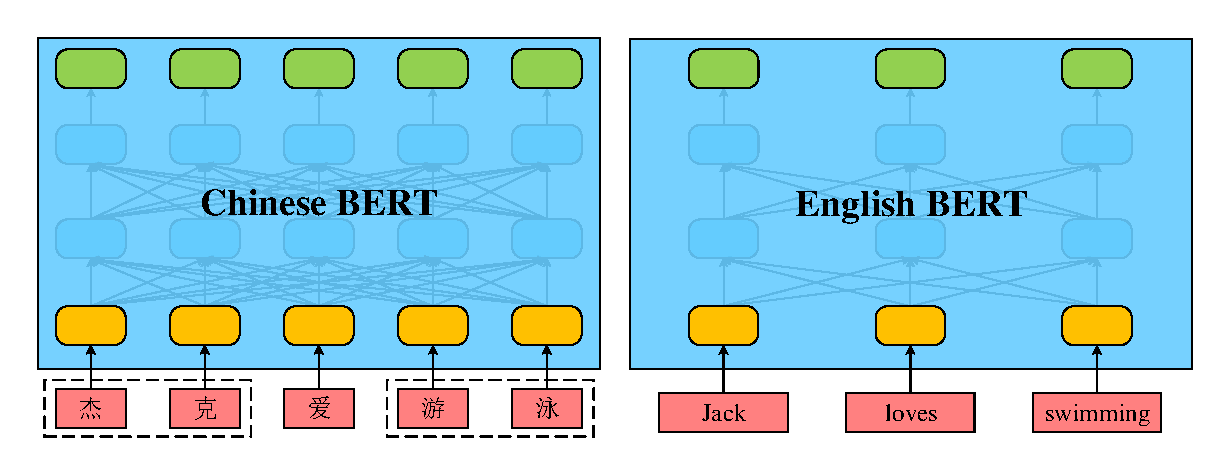
\includegraphics[width=0.98\textwidth]{figures/zh-vs-en-bert.pdf}
	\bicaption[fig:zh-vs-en-bert]{}{中文BERT(左)与英文BERT(右)对比示意图}{Fig.$\!$}{Comparison between Chinese BERT (left) and English BERT (right).}
\end{figure}

与其他大部分语言不同的是,在中文上,以BERT为代表的预训练模型往往使用字而不是词片段作为基本输入单元。
而由于中文中很大一部分词都是由超过一个字组成的,在中文预训练模型中,一个词由多个基本单元组成的现象十分常见。
图\ref{fig:zh-vs-en-bert}给出了中文BERT与英文BERT的对比示意图,对于句子“杰克爱游泳”(“Jack loves swimming”),在中文BERT上三个词中有两个词都被切分成了基本输入单元字,而在英文BERT上,三个词都没有被切分成词片段。

为了进一步证明这一点,本节在CoNLL 2009\cite{hajic-etal-2009-conll}多语言语义角色标注数据集上统计了各个语言的训练集中多基本单元词(由多个基本输入单元组成的词)所占的比例,结果如表\ref{tbl:multi-unit-word}所示。
结果表明,中文上的多基本单元词所占的比例超过了总词数的一般,要远高于其它语言。
在其他语言中,多基本单元词比例最高的德语中也仅有21\%的词由多个基本输入单元组成。
该发现充分说明了在中文预训练模型中,作为基本输入单元的字之间的关系的重要性。
因此,本章提出基于字级别依存关系的强化预训练模型,将这种重要的字间关系融入预训练模型中,从而增强其表示能力。

\begin{table}[htpb]
    \bicaption[tbl:multi-unit-word]{}{CoNLL 2009各语言训练集数据}{Table$\!$}{Training set statistics of different languages in CoNLL 2009.}
    \vspace{0.5em}\centering\wuhao
    \begin{tabular}{lccc}
        \toprule[1.5pt]
        语言 & 句子数 & 词数 & 多基本单元词比例\%  \\
        \midrule[1pt]
        中文  & 22,277  & 609,060  & 53.21 \\
        英文  & 39,279  & 958,167  & 14.37 \\
        德语   & 36,020  & 648,677  & 21.00 \\
        西班牙语 & 14,329  & 427,442  & 12.45 \\
        \bottomrule[1.5pt]
    \end{tabular}
\end{table}

最近,El Boukkouri等人\cite{el-boukkouri-etal-2020-characterbert}提出了一个基于字母的英文BERT,与基于词片段的英文BERT相比,其中可能存在更多的多基本单元。
他们仅仅在英文上训练了这种基于字母的BERT,而对于其他很多语言,现有的预训练模型基本都还是基于词片段的。
此外,由于本文的主要研究内容是中文语义依存图的应用,且目前自然语言处理领域绝大部分研究者仍然在英文等其他语言上使用基于词片段的预训练模型,而在中文上使用基于字的预训练模型,本章将集中研究中文的预训练模型和依存结构和融合方法。

\subsection{字级别依存关系强化网络}[Character-Level Dependency-Enhanced Network]
\label{sec:chapter5-char-level-dep-infusion}

\begin{figure}[hbtp]
	\centering
	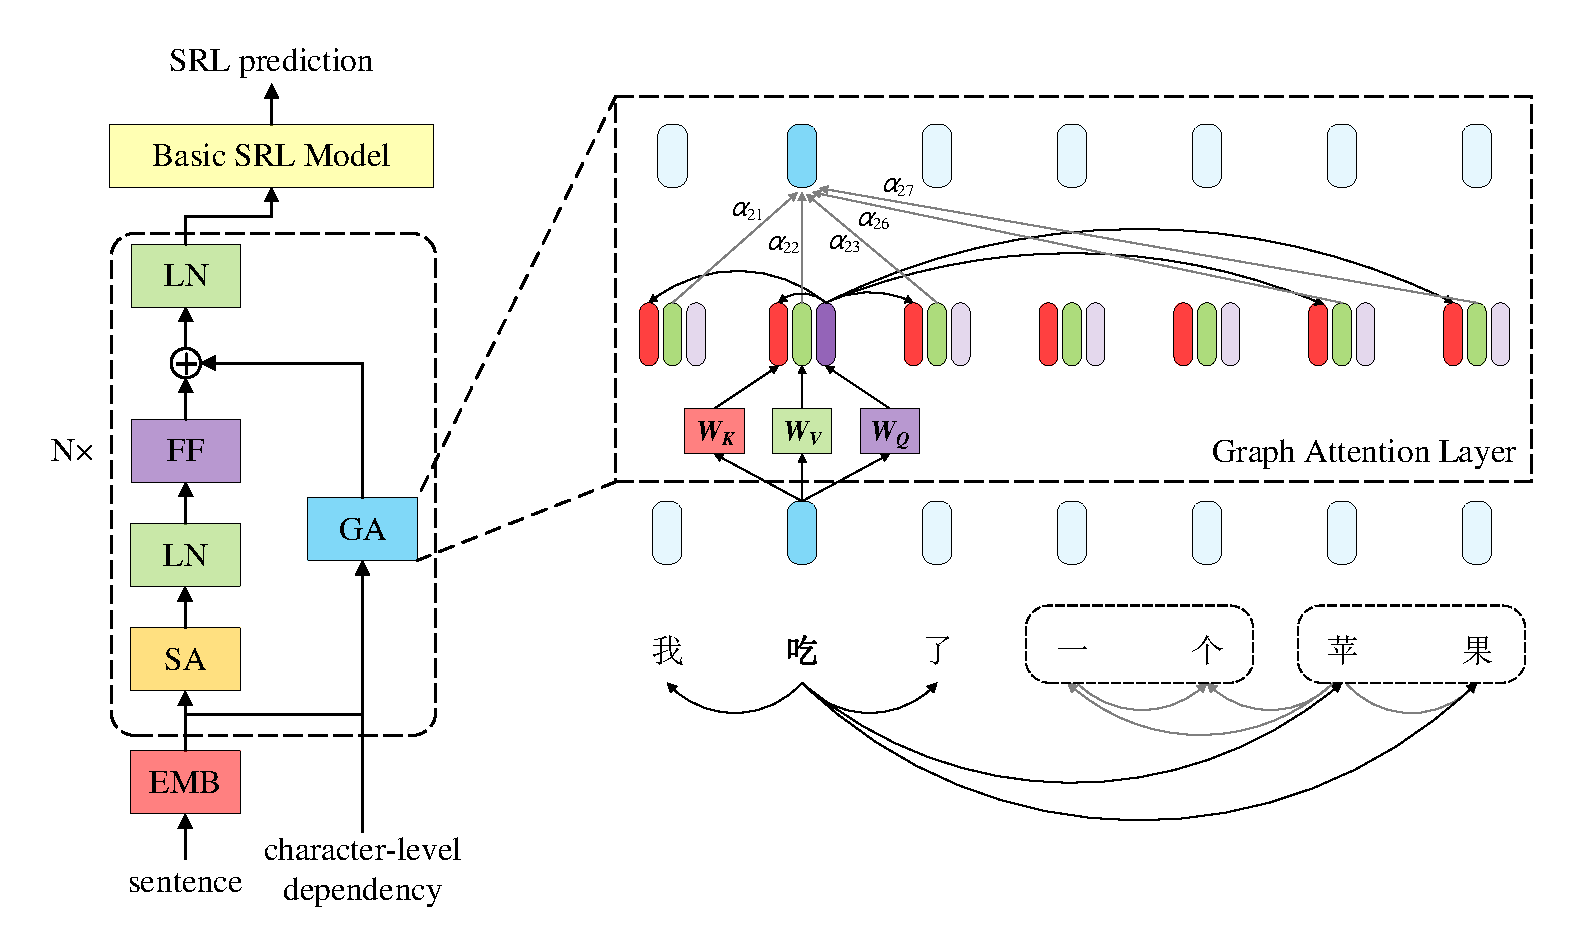
\includegraphics[width=0.95\textwidth]{figures/dependency-enhanced-network.pdf}
	\bicaption[fig:dependency-enhanced-network]{}{字级别依存关系强化网络结构示意图}{Fig.$\!$}{Character-Level Dependency-Enhanced Network.}
\end{figure}

本节将具体介绍本章提出的字级别依存关系强化网络,其结构如图\ref{fig:dependency-enhanced-network}所示。
该模型建立在中文BERT模型的基础上,图中EMB表示输入字向量(embeddings),SA表示自注意力层(self-attention layer),LN表示层标准化(layer normalization),FF表示前馈层(feed-forward layer),而GA表示图注意力层(graph attention layer)。

图注意力网络\cite{velickovic-etal-2018-gat}(Graph Attention Network,简称GAT)是自注意力网络的一种变体,通过注意机制将图结构融入神经网络中,模型中的图注意力层使用图注意力网络将字级别依存关系融入到预训练模型每一层。
具体来说,假设$\bm{h}_i$表示输入第$i$个字的隐层状态,图注意力网络首先计算各个字之间的相关分数:
\begin{equation}
    \label{eq:inter-score}
    s_{ij} = (\bm{h}_i\bm{W}_Q)(\bm{h}_j\bm{W}_K)^{\top}
\end{equation}
其中$\bm{h}_i\bm{W}_Q$和$\bm{h}_j\bm{W}_K$分别被称为查询(query)向量和键(key)向量,它们的乘积表示第$i$个字和第$j$个字之间的相关分数。
之后,该网络使用上述分数计算注意力分数:
\begin{equation}
\label{eq:att-score}
	\alpha_{ij} =\frac{\exp(s_{ij})}{\sum_{k\in\mathcal{N}_i}\exp(s_{ik})}
\end{equation}
其中$\mathcal{N}_i$表示第$i$个字在依存图中的邻居节点。
最后,第$i$个字经过依存图强化的输出为:
\begin{equation}
    \label{eq:gat-output}
	\bm{g}_i =\sum_{j\in \mathcal{N}_i}\alpha_{ij}(\bm{h}_j\bm{W}_V)
\end{equation}
其中$\bm{h}_j\bm{W}_V$称为值(value)向量。
假设将所有输入字的隐层状态拼接起来表示为$\bm{H} = [\bm{h}_1;\bm{h}_2; \dots; \bm{h}_n]$,而图注意力层输出的每个字的表示拼接起来表示为$\bm{G} = [\bm{g}_1;\bm{g}_2; \dots; \bm{g}_n]$,则上述图注意力层记为$\bm{G} = \text{GA}(\bm{H})$。

对于整个模型来说,其第$n$层的隐层状态$\bm{H}^n$通过如下方式计算:
\begin{equation}
	\label{eq:multi-att}
	\bm{A}^n = \text{LN}(\text{MultiAttn}(\bm{H}^{n-1}) + \bm{H}^{n-1})
\end{equation}
\begin{equation}
	\label{eq:ff}
	\bm{H}^n = \text{LN}(\text{FF}(\bm{A}^{n}) + \bm{A}^{n} + \text{GA}(\bm{H}^{n-1}))
\end{equation}
其中LN表示层标准化,$\bm{H}^0$表示输入字向量,而最高层隐层表示$\bm{H}^N$作为该模型输出的包含字级别依存信息的字表示,被输入其他任务的模型。
其中MultiAttn表示多头自注意力层,是由多个自注意力网络(SA)拼接而成,每个自注意力网络计算方式与公式\ref{eq:inter-score},\ref{eq:att-score}和\ref{eq:gat-output}中的图注意力网络计算方式基本相同,只是在计算最终输出时要考虑当前字与所有字而不是只与其相邻字之间的关系,需要将公式\ref{eq:gat-output}变为:
\begin{equation}
    \label{eq:sa-output}
	\bm{h}_i =\sum_{j=1}^{n}\alpha_{ij}(\bm{h}_j\bm{W}_V)
\end{equation}
另外公式\ref{eq:ff}中的FF表示前馈层:
\begin{equation}
    \text{FF}(\bm{h}) = \text{GELU}(\bm{W}\bm{h} + \bm{b})
\end{equation}
其中GELU为激活函数。

\subsection{字级别依存关系构建}[Construction of Character-Level Dependencies]

第\ref{sec:chapter5-char-level-dep-infusion}节中介绍的字级别依存关系强化网络需要输入序列的字级别依存关系作为额外信息输入,但目前词级别依存关系标注无论在句法还是语义任务上都占据主流,因此接下来首要的问题是如何在现有的词级别依存关系基础上构建字级别依存图。

具体的,给定输入句子$X = \{w_1, w_2, \dots, w_n\}$,其中$w_i$表示第$i$个词,该句子的词级别依存结构(句法依存树或语义依存图)为$G_w(X)$。
$w_i \rightarrow w_j \in G_w(X)$表示$G_w(X)$中存在一条从$w_i$指向$w_j$的弧。
假设一个词$w_i$中包括$m$个字,即$w_i=\{c_{i1}, c_{i2}, \dots, c_{im}\}$。
首先生成词内弧(intra-word arcs),即包含每个词内各个字之间依存关系的弧。
将每个词中的第一个字视为其中心节点,然后加入由第一个字指向后面所有字的弧。
具体来说,对于词$w_i$,向字级别依存图$G_c(X)$中加入第一个词$c_{i1}$指向后面每个字$c_{i2}, \dots, c_{im}$的弧,即$c_{i1} \rightarrow c_{i2} \in G_c(X), \dots, c_{i1} \rightarrow c_{im} \in G_c(X)$。

接下来生成词间弧(inter-word arcs),即包含各词之间依存关系的弧。
对于$G_w(X)$中的弧$w_i \rightarrow w_j \in G_w(X)$,向字级别依存图$G_c(X)$中加入由其中的父节点$w_i$的第一个字$c_{i1}$指向其中的子节点$w_j$中的每一个字$c_{j1}, \dots, c_{jm}$的弧。
记为$c_{i1} \rightarrow c_{j1} \in G_c(X), \dots, c_{i1} \rightarrow c_{jm} \in G_c(X)$。

\begin{figure}[hbtp]
	\centering
	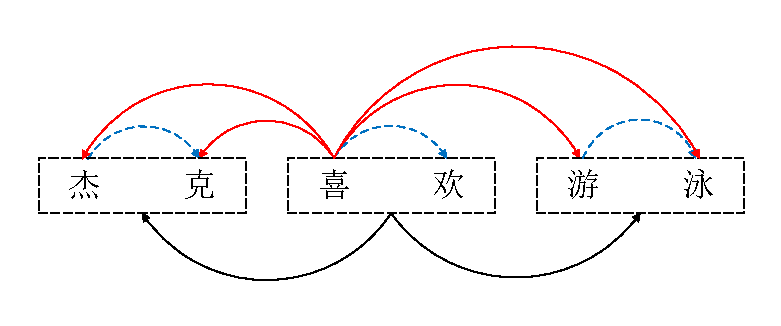
\includegraphics[width=0.75\textwidth]{figures/word-to-char.pdf}
	\bicaption[fig:word-to-char]{}{词级别(下)与字级别(上)依存关系转换示意图}{Fig.$\!$}{Converting word-level (lower) dependencies to character-level (upper).}
\end{figure}

图\ref{fig:word-to-char}中给出了从词级别依存关系转换为字级别依存关系的示意图,其中下方表示原始的词级别依存弧,上方红色实线表示字级别词间弧,蓝色虚线表示字级别词内弧。
由于在生成两种字级别依存弧的时候本章都选取了每个词的第一个字作为核心节点,每个词内的各个字的信息也通过词内弧传递到了第一个字,因此最终输出时使用每个词第一个字的隐层状态作为整个词的表示向量。


\section{字级别依存关系强化网络的应用}[Application of Character-Level Dependency-Enhanced Network]

本章第\ref{sec:chapter5-char-level-dep-infusion}节中介绍的字级别依存关系强化网络能有效将依存结构(句法依存树或语义依存图)融入预训练模型,从而获取结构信息强化的上下文相关词表示。
在此基础上,只需要使用前馈网络和softmax分类器等简单的神经网络模块就能完成很多自然语言处理任务,并有效提高预训练模型的性能。
本节将分别对基于强化预训练模型的命名实体识别和关系抽取模型进行介绍。

\subsection{命名实体识别上的应用}[Application on Semantic Role Labeling]
\label{sec:chapter5-srl-model}

根据语义角色定义的不同,语义角色标注(Semantic Role Labeling,简称SRL)任务可以分为两类,即基于段的(span-based)语义角色标注和基于词的(word-based)语义角色标注。
其中前者使用多个连续的词组成的段作为语义角色,而后者则使用单个词作为语义角色。
本节选择基于词的语义角色标注作为目标任务,并使用CoNLL 2009\cite{hajic-etal-2009-conll}语义角色标注公开评测中的中文部分进行实验。

\begin{figure}[htbp]
	\centering
	\begin{dependency}[arc edge, arc angle=80, text only label, label style={above}]
	    \tikzstyle{label}=[draw=black, text=black, fill=blue!30, inner sep=1ex, rounded corners]
		\begin{deptext}[column sep=1.5em, row sep=.5ex]
		    昨天\&      ,\& 我\& 吃\&  了\& 一个\& 苹果\\
		    |[label]| AM-TMP\&     \& |[label]| A0\& |[label]| 吃.01\& \&   \& |[label]| A1\\
		\end{deptext}
		\deproot[edge unit distance=3ex]{4}{root}
		\depedge{4}{1}{adv}
		\depedge{4}{2}{punc}
		\depedge{4}{3}{subj}
		\depedge{4}{5}{adjct}
		\depedge{4}{7}{obj}
		\depedge{7}{6}{adv}
	\end{dependency}
	\bicaption[fig:srl-example]{}{语义角色标注(下)和句法依存树(上)示意图}{Fig.$\!$}{Example of SRL annotation (lower) and syntactic dependency tree (upper).}
\end{figure}

图\ref{fig:srl-example}中给出了一个句子的语义角色标注和句法依存树示意图。
语义角色标注一般分为四个子任务:

1. 谓词识别(predicate identification):识别出作为句子中心词的谓词。
在例子中即识别出“吃”为谓词。
在复杂的句子中可能存在多个谓词。

2. 谓词消歧(predicate disambiguation):找到句中谓词合适的语义(sense)。
在例子中即识别出谓词“吃”的语义为定义中的第一个“吃.01”。

3. 论元识别(argument identification):对于句中每一个谓词,识别出与其语义相关的论元。
在例子中即识别谓词“吃”的论元包括“昨天”、“我”和“苹果”。

4. 论元分类(argument classification):对于句中每一个谓词和论元对,对其关系进行分类。
在例子中即将谓词“吃”和其论元“我”的关系抽取为A0,将“吃”和“苹果”的关系抽取为A1,将“吃”和“昨天”的关系抽取为AM-TMP。

在CoNLL 2009评测中,每个句子的论元已经给定,也就是说不需要模型实现上述子任务中的谓词识别,只需要实现另外三个子任务。
此外,论元识别和论元分类两个子任务一般通过序列标注方法一起实现。
具体来说,模型根据输入句子和当前谓词分别为句子中的每个词预测一个标签,该标签来自所有可能的谓词-论元关系组成的集合,其中也包括一个特别的空标签,用于表示该词和当前谓词之间没有关系。
通过这种序列标注的方式,就能同时完成对论元的识别和分类,因此将这两个任务合并后的任务称为论元标注(argument labeling)。

图\ref{fig:pipeline-srl-model}中给出了本章使用的语义角色标注模型示意图。
其中包括两部分,分别用于处理谓词消歧和论元识别及分类。
上方模型为谓词消歧模型,其首先通过本章提出的字级别依存关系强化网络获取每个词的向量表示,然后通过一个简单的前馈网络和softmax分类器预测句子中每个谓词的语义:
\begin{equation}
    p(s|\bm{h}_i) = \text{softmax}(\bm{W}\bm{h}_i + \bm{b})
\end{equation}
其中$\bm{h}_i$为第$i$个词的表示向量,$p(s|\bm{h}_i)$表示其标签为$s$的概率。

\begin{figure}[hbtp]
	\centering
	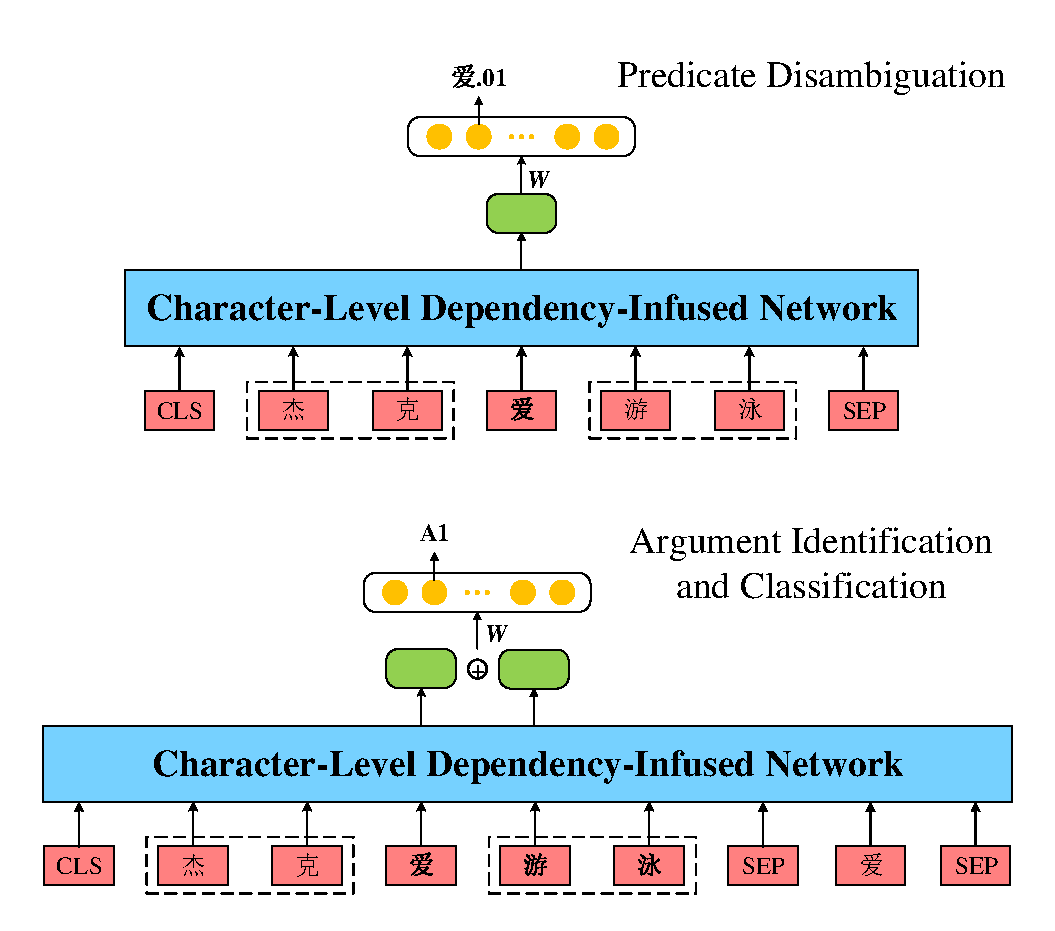
\includegraphics[width=0.85\textwidth]{figures/pipeline-srl-model.pdf}
	\bicaption[fig:pipeline-srl-model]{}{语义角色标注模型示意图}{Fig.$\!$}{Semantic role labeling model.}
\end{figure}

图\ref{fig:pipeline-srl-model}中下方模型为论元识别及分类模型,对于句中每个谓词,其首先将该谓词拼接到句子最后,用特殊符号“[SEP]”隔开。
也就是说对于每个谓词,该模型输入为:“[CLS] 句子 [SEP] 谓词 [SEP]”。
其中“[CLS]”和“[SEP]”都是BERT模型训练时使用的特殊符号,“[CLS]”作为句子开头符号,“[SEP]”则用于分开两个句子和表示句子结尾。
通过这种组合方式,句中其他词可以更好地获取当前谓词的信息。
之后通过本章提出的字级别依存关系强化网络获取每个词的向量表示,将当前谓词的向量和其他每一个词的向量分别进行拼接,然后通过一个前馈网络和softmax分类器预测当前谓词和其他词之间的语义关系:
\begin{equation}
    p(r|\bm{h}_p,\bm{h}_j) = \text{softmax}(\bm{W}[\bm{h}_p;\bm{h}_j)] + \bm{b})
\end{equation}
其中$\bm{h}_p$为当前谓词的表示向量,$\bm{h}_j$为句中第$j$个词的表示向量,$p(r|\bm{h}_p,\bm{h}_j)$表示第$j$个词与当前谓词间语义关系为$r$的概率。
在语义标签的集合中,有一个额外的“O”标签,用于表示当前词与谓词之间无关系。

\subsection{关系抽取上的应用}[Application on Relation Extraction]
\label{sec:chapter5-re-model}

关系抽取(Relation Extraction,简称RE)任务目的是预测句中给定的两个实体间的关系,该任务对于构建知识图谱有重要意义。
例如对于句子“我抬头看天”,给定两个实体分别为“我”和“头”,该任务需要预测二者的关系为Part-Whole,即部分与整体关系。

\begin{figure}[hbtp]
	\centering
	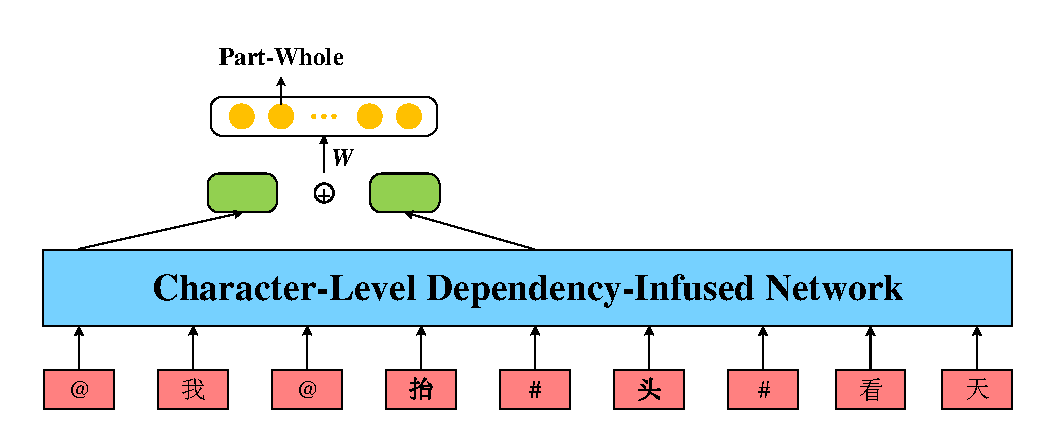
\includegraphics[width=0.85\textwidth]{figures/re-model.pdf}
	\bicaption[fig:re-model]{}{关系抽取模型示意图}{Fig.$\!$}{Relation Extraction model.}
\end{figure}

图\ref{fig:re-model}中给出了本章使用的关系抽取模型示意图。
具体来说,该模型首先在句中第一个实体的前后加上特殊符号“@”,然后在句中第二个实体的前后加上特殊符号“\#”。
经过这种修改,上述例句变为“@我@抬\#头\#看天”。
接着,将修改后的句子输入本章提出的字级别依存关系强化网络获取每个词的向量表示。
使用第一个实体前的“@”符号的向量作为其表示,使用第二个实体前的“\#”符号的向量作为其表示,然后拼接这两个向量,通过一个前馈网络和softmax分类器预测这两个实体之间的关系:
\begin{equation}
    p(r|\bm{h}_{@},\bm{h}_{\#}) = \text{softmax}(\bm{W}[\bm{h}_{@};\bm{h}_{\#})] + \bm{b})
\end{equation}
其中$\bm{h}_{@}$为第一个实体的表示向量,$\bm{h}_{\#}$为第二个实体的表示向量,$ p(r|\bm{h}_{@},\bm{h}_{\#})$表示两个实体间关系为$r$的概率。

\section{实验与分析}[Experiments and Analysis]

\subsection{实验设置}[Experimental Settings]

本章首先在CoNLL 2009语义角色标注数据集的中文部分测试了提出的字级别依存关系强化网络,然后又在SanWen和FinRE两个中文关系抽取数据集上测试了该网络。
这三个数据集的相关信息见表\ref{tbl:chapter5-statistics}。
其中CoNLL 2009数据集为基于字的语义角色标注数据集,其中已经预先给出了每句话中的所有谓词,只需要进行谓词消歧、论元识别及分类。

\begin{table}[htbp]
    \bicaption[tbl:chapter5-statistics]{}{语义角色标注和关系抽取数据集信息}{Table$\!$}{Statistics of Semantic Role Labeling and Relation Extraction dataset.}
    \vspace{0.5em}\centering\wuhao
    \begin{tabular}{lcccccc}
        \toprule[1.5pt]
        数据集 & 标签数 & 训练集 & 开发集 & 测试集 & 平均句子长度 \\
        \midrule[1pt]
        CoNLL 2009 & 37 & 22,277 & 1,762 & 2,556 & 27.52 \\
        SanWen     & 9  & 17,227 & 1,793 & 2,220 & 89.41 \\
        FinRE      & 43 & 13,486 & 1,489 & 3,727 & 143.62 \\
        \bottomrule[1.5pt]
    \end{tabular}
\end{table}

在CoNLL 2009数据集上的实验中,本章分别使用了句法依存树和语义依存图作为输入到模型的额外依存关系。
其中分别尝试了模型预测的和人工标注的句法依存树,均由CoNLL 2009公开评测官方提供。
而由于CoNLL 2009数据集上没有人工标注的语义依存图,本章只使用了模型预测的语义依存图作为额外输入。
用于预测的模型为在SemEval 2016 Task 9中文语义依存图中的两个数据集上训练的Biaffine依存图分析器。
在该数据集上,本章与以下模型进行了对比:

\begin{itemize}
    \item \citet{roth-lapata-2016-neural}:该模型将句法树上的路径转化为向量向神经网络中加入句法信息。
    \item \citet{marcheggiani-etal-2017-simple}:该模型将双向LSTM应用到语义角色标注任务中。
    \item \citet{he-etal-2018-syntax}:该模型使用人工标注句法信息帮助模型进行论元剪枝,删除不可能的论元从而提高预测准确率。
    \item \citet{he-etal-2019-syntax}:该模型在使用句法信息进行论元剪枝的基础上还使用了预训练模型BERT获取上下文相关词向量作为输入。
    \item \citet{li-etal-2018-unified}:该模型使用图卷积网络将句法信息直接融入神经网络中。
    \item \citet{munir-etal-2021-adaptive}:该模型使用适应性卷积网络和Tree-LSTM将句法信息直接融入神经网络。
    \item \citet{xia-etal-2019-syntax}:该模型使用多任务学习框架同时学习句法分析任务和语义角色标注,从而隐式地将句法信息通过共享的参数传递给语义角色标注任务。
    \item \citet{li-etal-2020-high}:该模型在预训练模型的基础上将高维图结构特征引入模型中,进一步提高了模型性能。
    \item BERT:本章实现的使用BERT模型作为输入的基线模型,没有使用额外的结构化信息。
    \item BERT + Word-Level GCN:本章实现的在BERT模型基础上用图卷积网络融入词级别句法信息的基线模型。
\end{itemize}

在SanWen和FinRE两个关系抽取数据集上,本章使用了预测的语义依存图作为额外输入。
用于预测的模型与CoNLL 2009实验中用到的相同。
在关系抽取任务上,本章与以下模型进行了对比:
\begin{itemize}
    \item \citet{xu-etal-2020-chinese}:该模型使用网格门控循环神经⽹络(lattice gated recurrent neural network)对句子进行建模。
    \item \citet{zhang-yu-2020-chinese}:该模型使用了网格LSTM网络对输入句子进行建模,同时还使用了BERT作为其输入。
    \item \citet{li-etal-2019-chinese}:该模型使用了多粒度网格网络(multi-grained lattice framework)对输入句子进行建模,同时还使用了来自知网的外部数据作为额外信息。
    \item BERT:本章实现的使用BERT模型作为输入的基线模型,没有使用额外的结构化信息。
\end{itemize}

在训练过程中,本章分别使用中文预训练模型BERT和RoBERTa对本章提出的字级别依存关系强化网络的参数进行初始化。
使用AdamW算法\cite{loshchilov-hutter-2019-decoupled}优化参数,并将初始学习率设置为2e-5。

本章在语义角色标注实验中使用的评价指标包括精确率(P)、召回率(R)、F1值(F1)以及谓词消歧子任务的准确率(ACC)。
而在关系抽取任务上使用F1值(F1)作为评价指标。

\subsection{语义角色标注实验结果}[Results on Semantic Role Labeling]


\begin{table}[htpb]
    \bicaption[tbl:srl-result]{}{CoNLL 2009中文数据集上语义角色标注实验结果}{Table$\!$}{Chinese Semantic Role Labeling results on CoNLL-2009.}
    \vspace{0.5em}\centering\wuhao
    \begin{tabular}{lccccc}
        \toprule[1.5pt]
        模型 & BERT & 结构信息 & P & R & F1 \\
        \midrule[1pt]
        \citet{roth-lapata-2016-neural}       & & \checkmark & 83.2 & 75.9 & 79.4 \\
        \citet{marcheggiani-etal-2017-simple} & & & 83.4 & 79.1 & 81.2 \\
        \citet{he-etal-2018-syntax}           & & \checkmark & 84.2 & 81.5 & 82.8 \\
        \citet{li-etal-2018-unified}          & & \checkmark & 84.8 & 81.2 & 83.0 \\
        \citet{he-etal-2019-syntax}           & & \checkmark & 84.6 & 84.5 & 84.6 \\
        \citet{munir-etal-2021-adaptive}      & & \checkmark & 84.7 & 85.1 & 84.9 \\
        \citet{xia-etal-2019-syntax}          & & \checkmark & 84.6 & 85.7 & 85.1 \\
        \citet{he-etal-2019-syntax}           & \checkmark & \checkmark & 86.2 & 86.7 & 86.4 \\
        \citet{xia-etal-2019-syntax}          & \checkmark & \checkmark & 88.0 & 89.1 & 88.5 \\
        \citet{li-etal-2020-high}             & \checkmark & & -	& - & 88.7 \\
        BERT                                  & \checkmark & & 88.2 & 88.3 & 88.2 \\
        BERT + Word-Level GCN                 & \checkmark & \checkmark & 88.6 & 88.5 & 88.5 \\
        Ours + Syntax                         & \checkmark & \checkmark & 89.2 & 88.5 & 88.9 \\
        Ours + SDG                            & \checkmark & \checkmark & 89.1 & 88.7 & 88.9 \\
        Ours + Syntax + SDG                   & \checkmark & \checkmark & 89.2 & 89.0 & 89.1 \\
        \bottomrule[1.5pt]
    \end{tabular}
\end{table}

表\ref{tbl:srl-result}中列出了CoNLL 2009语义角色标注中文数据集上的实验结果,表中使用对号显示了每个模型是否使用BERT作为输入以及是否使用了结构信息(句法依存树或语义依存图)作为输入。
其中所列本章提出的模型包括:
\begin{itemize}
    \item Ours + Syntax:本章提出的字级别依存关系强化的预训练BERT模型,使用句法依存树作为结构化信息输入。
    \item Ours + SDG:本章提出的字级别依存关系强化的预训练BERT模型,使用语义依存图作为结构化信息输入。
    \item Ours + Syntax + SDG:本章提出的字级别依存关系强化的预训练BERT模型,同时使用句法依存树和语义依存图作为结构化信息输入,在模型每一层使用两个独立的图注意力网络分别对句法依存树和语义依存图进行建模,然后将结果相加。
\end{itemize}

从表中结果可以发现,使用BERT作为输入的模型在性能上普遍显著超过了不使用BERT的模型。
本章实现的只使用BERT的基线模型已经超过了大部分此前的方法的结果。
另外,本章实现的另一个使用图卷积网络将词级别句法信息融入BERT输出的基线模型,在BERT模型的基础上获得了性能提升。
而本章提出的字级别依存关系强化的预训练BERT模型则取得了目前最好结果。
值得注意的是,分别使用句法依存树和语义依存图作为输入时,获取了基本相同的最好结果。
为了进一步探索句法依存树和语义依存图对于该任务的帮助是否是重复、可以相互替代的,本章又尝试了同时将句法依存树和语义依存图作为模型的结构信息输入,在每一层使用两个独立的图注意力网络对它们分别建模,然后将二者的隐层状态相加。
实验结果表明,同时使用句法依存树和语义依存图作为输入时,模型性能得到进一步提升。
这也说明了二者为模型提供的是不同类型的信息。

\begin{table}[htpb]
    \bicaption[tbl:srl-result-sub-task]{}{CoNLL 2009中文数据集上语义角色标注子任务实验结果}{Table$\!$}{Chinese Semantic Role Labeling sub-task results on CoNLL-2009.}
    \vspace{0.5em}\centering\wuhao
    \begin{tabular}{lcccc}
        \toprule[1.5pt]
        \multirow{2}{*}{模型}& \multicolumn{3}{c}{论元标注} & 谓词消歧 \\
        \cmidrule(r){2-4} \cmidrule(r){5-5}
         & P & R & F1 & ACC \\
        \midrule[1pt]
        BERT                   & 84.6 & 84.8 & 84.7 & 96.3 \\
        BERT + Word-Level GCN  & 85.2 & 85.0 & 85.1 & 96.3 \\
        Ours + Syntax          & 86.1 & 85.1 & 85.6 & 96.2  \\
        Ours + SDG             & 85.8 & 85.3 & 85.6 & 96.3 \\
        Ours + Syntax + SDG    & 86.1 & 85.8 & 86.0 & 96.2  \\
        \bottomrule[1.5pt]
    \end{tabular}
\end{table}

根据第\ref{sec:chapter5-srl-model}节的介绍,CoNLL 2009语义角色标注任务包括两个子任务:谓词消歧和论元标注(论元识别和分类)。
为了分析本章提出的方法对各个子任务的影响,本章在表\ref{tbl:srl-result-sub-task}中列出了本章模型在各子任务上的结果。
根据表中信息可以发现,所有模型在谓词消歧上都取得了相差不大的结果,这很可能是因为该任务是一个较简单的任务,且其准确率已经很高,加入额外结构信息也无法对其产生帮助。
而本章提出的模型为语义角色标注任务带来的性能提升主要来自论元标注子任务。
可以发现,在消除了谓词消歧性能的影响后,本章提出的模型带来的性能提升变得更为明显。

\begin{table}[htpb]
    \bicaption[tbl:srl-result-with-gold]{}{CoNLL 2009数据集上使用人工标注句法树的实验结果}{Table$\!$}{Results on CoNLL-2009 with gold syntactic trees.}
    \vspace{0.5em}\centering\wuhao
    \begin{tabular}{lccccc}
        \toprule[1.5pt]
        模型 & P & R & F1 \\
        \midrule[1pt]
        BERT                               & 88.2 & 88.3 & 88.2 \\
        BERT + Word-Level GCN (Predicted)  & 88.6 & 88.5 & 88.5 \\
        BERT + Word-Level GCN (Gold)       & 90.8 & 90.3 & 90.5 \\
        Ours + Syntax (Predicted)          & 89.2 & 88.5 & 88.9 \\
        Ours + Syntax (Gold)               & 91.9 & 91.8 & 91.9 \\
        \bottomrule[1.5pt]
    \end{tabular}
\end{table}

为了进一步探索本章提出的字级别依存关系强化模型的上限,本章尝试用人工标注的正确句法树(Gold)替换此前实验中使用的模型预测的句法树(Predicted)输入模型中。
由于在CoNLL 2009数据集上只有句法依存树的人工标注,而没有语义依存图的人工标注,这里只尝试了使用人工标注句法树作为输入。
该实验结果如表\ref{tbl:srl-result-with-gold}所示。
根据表中结果可以发现,当使用人工标注的正确句法树替换模型预测句法树时,无论是本章提出的模型还是使用词级别依存关系的基线模型的性能都获得了显著提升。
而其中本章提出的模型的性能提升比基线模型更加明显,且使用正确句法树时,本章提出的模型性能与基线模型的性能差距变得更大。
这说明了本章提出的模型有更高的上限。

\begin{table}[h]
    \bicaption[tbl:srl-result-subtract]{}{CoNLL 2009数据集上使用不同依存弧的实验结果}{Table$\!$}{Results on CoNLL-2009 with different sets of dependency arcs.}
    \vspace{0.5em}\centering\wuhao
    \begin{tabular}{lcccc}
        \toprule[1.5pt]
        模型 & 句法信息 & P & R & F1\\
        \midrule[1pt]
        BERT & - & 84.7 & 84.9 & 84.8 \\
        Ours + Syntax & Predicted & 86.0 & 85.0 & 85.5 (+0.7) \\
        Ours + Syntax & Gold $\cap$ Predicted & 87.5 & 86.8 & 87.1 (+2.3) \\
        Ours + Syntax & Gold $\setminus$ Predicted & 88.1 & 87.0 & 87.6 (+2.8) \\
        Ours + Syntax & Gold & 90.3 & 90.1 & 90.2 (+5.4)  \\
        \bottomrule[1.5pt]
    \end{tabular}
\end{table}

接下来,为了更深入的探索模型预测句法树和人工标注的正确句法树对本章提出模型的影响,本章使用了不同集合的依存弧作为输入,实验结果如表\ref{tbl:srl-result-subtract}所示。
由于加入依存信息不会影响谓词消歧子任务的结果,同时为了更清晰地显示出模型之间的差距,表中所列结果是论元标注子任务的结果。
而其中F1值括号里的值表示的是该模型相对BERT基线模型的性能提升。
其中“Gold $\cap$ Predicted”表示模型预测的句法树中正确的弧组成的集合,可以认为这个集合中的弧是容易预测的。
根据CoNLL 2009官方提供的模型预测句法树的准确率,这部分弧占总数的82.6\%。
而“Gold $\setminus$ Predicted”表示人工标注的句法树中不在模型预测的句法树中的弧组成的集合,也就是说模型错误预测了这些弧。
可以认为这个集合中的弧是难以预测正确的,占弧总数的17.4\%。
根据实验结果可以发现,不到五分之一的难以预测的弧为模型带来的性能提升反而比约占五分之四的容易预测的弧多。
该实验说明了目前依存分析器预测错误的少数依存弧中还蕴涵大量对于语义角色标注有帮助的信息,而只要能提升依存分析器的性能,将这些信息加入本章提出的模型,就能够获得更显著的性能提升。

\subsection{关系抽取实验结果}[Results on Relation Extraction]


\begin{table}[htpb]
    \bicaption[tbl:re-result]{}{FinRE和SanWen数据集上关系抽取实验结果}{Table$\!$}{Relation Extraction results on FinRE and SanWen.}
    \vspace{0.5em}\centering\wuhao
    \begin{tabular}{lc}
        \toprule[1.5pt]
        模型 & F1 \\
        \midrule[1pt]
        \multicolumn{2}{c}{SanWen} \\
        \hline
        \citet{xu-etal-2020-chinese} & 57.43 \\
        \citet{zhang-yu-2020-chinese} & 63.13 \\
        \citet{li-etal-2019-chinese} & 65.61 \\
        BERT & 76.75 \\
        BERT + SDG & \bf 77.73 \\
        \hline
        \multicolumn{2}{c}{FinRE} \\
        \hline
        Li et al. & 49.26 \\
        BERT & 56.82 \\
        BERT + SDG & \bf 57.26 \\
        \bottomrule[1.5pt]
    \end{tabular}
\end{table}

表\ref{tbl:re-result}中列出了在SanWen和FinRE两个中文关系抽取数据集上的实验结果。
在该任务上,由于没有人工标注的句法依存树或语义依存图,本章只使用了模型预测的语义依存图作为本章提出的字级别依存关系强化模型的输入。
另外,如第\ref{sec:chapter5-re-model}节中所介绍,本章使用的关系抽取模型首先在两个实体前后加入特殊符号,然后将修改后序列输入字级别依存关系强化模型,最后直接拼接两个特殊符号的输出向量通过前馈网络和softmax分类器预测实体间的关系。
该方法适于应用在基于字的预训练模型上,但比较难与基于词的依存信息融合方法一起使用。
因此本章只对比了此前的工作、使用BERT的基线模型和本章提出的的字级别依存关系强化模型的结果。

根据表中结果可以发现,本章实现的基于BERT的基线模型的性能已经远好于此前几个工作提出的模型。
而在此基础上,本章提出的字级别依存关系强化模型在使用模型预测的语义依存图作为输入时在两个数据集上都取得了明显的性能提升。

\section{本章小结}[Conclusions]

本章针对中文语义依存图在其他自然语言处理任务中的应用问题,结合中文预训练模型使用字级别输入的特点,设计了字级别依存关系强化网络,将字级别的依存信息与预训练模型紧密结合,从而获取包含字级别依存信息的上下文相关表示向量,作为其他任务的输入。
为了证明该模型的有效性,本章在中文语义角色标注和关系抽取任务上进行了实验。
实验表明,通过本章提出的字级别依存关系强化网络,中文语义依存图能有效帮助提升这两个任务上模型的性能。
并且语义依存图与句法依存树能为模型提供不同类型的结构信息,二者结合时能进一步提升模型性能。
本章提出的模型在中文语义角色标注和关系抽取任务上都取得了目前最好结果。


% Local Variables:
% TeX-master: "../thesis"
% TeX-engine: xetex
% End:
\backmatter
% !Mode:: "TeX:UTF-8" 
\begin{conclusions}

学位论文的结论作为论文正文的最后一章单独排写,但不加章标题序号。

结论应是作者在学位论文研究过程中所取得的创新性成果的概要总结,不能与摘要混为一谈。博士学位论文结论应包括论文的主要结果、创新点、展望三部分,在结论中应概括论文的核心观点,明确、客观地指出本研究内容的创新性成果(含新见解、新观点、方法创新、技术创新、理论创新),并指出今后进一步在本研究方向进行研究工作的展望与设想。对所取得的创新性成果应注意从定性和定量两方面给出科学、准确的评价,分(1)、(2)、(3)…条列出,宜用“提出了”、“建立了”等词叙述。

\end{conclusions}
   % 结论
\bibliographystyle{gbt7714-numerical}
\bibliography{reference}
%%%%%%%%%%%%%%%%%%%%%%%%%%%%%%%%%%%%%%%%%%%%%%%%%%%%%%%%%%%%%%%%%%%%%%%%%%%%%%%% 
%-- 注意:以下本硕博、博后书序不一致 --%
%%%%%%%%%%%%%%%%%%%%%%%%%%%%%%%%%%%%%%%%%%%%%%%%%%%%%%%%%%%%%%%%%%%%%%%%%%%%%%%% 
% 硕博书序
%%%%%%%%%%%%%%%%%%%%%%%%%%%%%%%%%%%%%%%%%%%%%%%%%%%%%%%%%%%%%%%%%%%%%%%%%%%%%%%% 
\begin{appendix}%附录
%% -*-coding: utf-8 -*-
%%%%%%%%%%%%%%%%%%%%%%%%%%%%%%%%%%%%%%%%%%%%%%%%%%%%%%%%%
\chapter{带章节的附录}[Full Appendix]%
完整的附录内容,包含章节,公式,图表等

%%%%%%%%%%%%%%%%%%%%%%%%%%%%%%%%%%%%%%%%%%%%%%%%%%%%%%%%%
\section{附录节的内容}[Section in Appendix]
这是附录的节的内容

附录中图的示例:
\begin{figure}[htbp]
\centering
\includegraphics[width = 0.4\textwidth]{golfer}
%\bicaption[golfer5]{}{\xiaosi[0]打高尔夫球的人}{Fig.$\!$}{The person playing golf}\vspace{-1em}
\caption{\xiaosi[0]打高尔夫球的人}
\end{figure}

附录中公式的示例:
\begin{align}
a & = b \times c \\
E & = m c^2
\label{eq}
\end{align}

\chapter{这个星球上最好的免费Linux软件列表}[List of the Best Linux Software in our Planet]
\section{系统}

\href{http://fvwm.org/}{FVWM 自从上世纪诞生以来,此星球最强大的窗口管理器。}
推荐基于FVWM的桌面设计hifvwm:\href{https://github.com/dustincys/hifvwm}{https://github.com/dustincys/hifvwm}。

\subsection{hifvwm的优点}

\begin{enumerate}
	\item 即使打开上百个窗口也不会“蒙圈”。计算机性能越来越强大,窗口任务的管理必须要升级到打怪兽级别。
	\item 自动同步Bing搜索主页的壁纸。每次电脑开机,午夜零点自动更新,用户
		也可以手动更新,从此审美再也不疲劳。
	\item 切换窗口自动聚焦到最上面的窗口。使用键盘快捷键切换窗口时候,减少
		操作过程,自动聚焦到目标窗口。这一特性是虚拟窗口必须的人性化设
		计。
	\item 类似window右下角的功能的最小化窗口来显示桌面的功能此处类似
		win7/win10,实现在一个桌面之内操作多个任务。
	\item 任务栏结合标题栏。采用任务栏和标题栏结合,节省空间。
	\item 同类窗口切换。可以在同类窗口之内类似alt-tab的方式切换。
	\item ……
\end{enumerate}

\section{其他}

\href{https://github.com/goldendict/goldendict}{goldendict 星球最强大的桌面字典。}

\href{https://github.com/yarrick/iodine}{iodine,“HIT-WLAN + 锐捷”时代的福音。}

\href{http://www.aircrack-ng.org/}{aircrack,Wifi“安全性评估”工具。}

\href{https://www.ledger-cli.org/}{ledger,前“金融区块链”时代最好的复式记账系统。}

\href{https://orgmode.org/}{orgmode,最强大的笔记系统,从来没有之一。}

\href{https://www.jianguoyun.com/}{坚果云,国内一款支持WebDav的云盘系统,国内真正的云盘没有之一。}

\href{http://www.mutt.org/}{mutt, ``All mail clients suck. This one just sucks less.''}

\section{vim}
实现中英文每一句一行,以及实现每一句折叠断行的简单正则式,tex源码更加乖乖。
\begin{lstlisting}
vnoremap <leader>fae J:s/[.!?]\zs\s\+/\="\r".matchstr(getline('.'), '^\s*')/g<CR>
vnoremap <leader>fac J:s/[。!?]/\=submatch(0)."\n".matchstr(getline('.'), '^\s*')/g<CR>
vnoremap <leader>fle :!fmt -80 -s<CR>
\end{lstlisting}

\end{appendix}
% !Mode:: "TeX:UTF-8" 
\begin{publication}
\noindent\textbf{发表的相关论文}

\begin{publist}
\item	XXX,XXX. Static Oxidation Model of Al-Mg/C Dissipation Thermal Protection Materials[J]. Rare Metal Materials and Engineering, 2010, 39(Suppl. 1): 520-524.(SCI~收录,IDS号为~669JS,IF=0.16)
\item XXX,XXX. 精密超声振动切削单晶铜的计算机仿真研究[J]. 系统仿真学报,2007,19(4):738-741,753.(EI~收录号:20071310514841)
\item XXX,XXX. 局部多孔质气体静压轴向轴承静态特性的数值求解[J]. 摩擦学学报,2007(1):68-72.(EI~收录号:20071510544816)
\item XXX,XXX. 硬脆光学晶体材料超精密切削理论研究综述[J]. 机械工程学报,2003,39(8):15-22.(EI~收录号:2004088028875)
\item XXX,XXX. 基于遗传算法的超精密切削加工表面粗糙度预测模型的参数辨识以及切削参数优化[J]. 机械工程学报,2005,41(11):158-162.(EI~收录号:2006039650087)
\item XXX,XXX. Discrete Sliding Mode Cintrok with Fuzzy Adaptive Reaching Law on 6-PEES Parallel Robot[C]. Intelligent System Design and Applications, Jinan, 2006: 649-652.(EI~收录号:20073210746529)
\end{publist}

\noindent\textbf{(二)申请及已获得的专利(无专利时此项不必列出)}
\begin{publist}
\item XXX,XXX. 一种温热外敷药制备方案:中国,88105607.3[P]. 1989-07-26.
\end{publist}

\noindent\textbf{(三)参与的科研项目及获奖情况}
\begin{publist}
\item	XXX,XXX. XX~气体静压轴承技术研究, XX~省自然科学基金项目.课题编号:XXXX.
\item XXX,XXX. XX~静载下预应力混凝土房屋结构设计统一理论. 黑江省科学技术二等奖, 2007.
\end{publist}

%\vfill
%\hangafter=1\hangindent=2em\noindent
%\setlength{\parindent}{2em}
\end{publication}
    % 所发文章
\include{back/ceindex}    % 索引, 根据自己的情况添加或者不添加,选择自动添加或者手工添加。
\authorization %授权
%\authorization[scan.pdf] %添加扫描页的命令,与上互斥
% !Mode:: "TeX:UTF-8"
\begin{acknowledgements}

Thank to \hithesis\ !


\end{acknowledgements}
 %致谢
% !Mode:: "TeX:UTF-8" 

\begin{resume}
XXXX~年~XX~月~XX~日出生于~XXXX。

XXXX~年~XX~月考入~XX~大学~XX~院(系)XX~专业,XXXX~年~XX~月本科毕业并获得~XX~学学士学位。

XXXX~年~XX~月------XXXX~年~XX~月在~XX~大学~XX~院(系)XX~学科学习并获得~XX~学硕士学位。

XXXX~年~XX~月------XXXX~年~XX~月在~XX~大学~XX~院(系)XX~学科学习并获得~XX~学博士学位。

获奖情况:如获三好学生、优秀团干部、X~奖学金等(不含科研学术获奖)。

工作经历:

\textbf{( 除全日制硕士生以外,其余学生均应增列此项。个人简历一般应包含教育经历和工作经历。)}
\end{resume}
          % 博士学位论文有个人简介
%%%%%%%%%%%%%%%%%%%%%%%%%%%%%%%%%%%%%%%%%%%%%%%%%%%%%%%%%%%%%%%%%%%%%%%%%%%%%%%% 
% 本科书序为:
%%%%%%%%%%%%%%%%%%%%%%%%%%%%%%%%%%%%%%%%%%%%%%%%%%%%%%%%%%%%%%%%%%%%%%%%%%%%%%%% 
% \authorization %授权
% % \authorization[scan.pdf] %添加扫描页的命令,与上互斥
% % !Mode:: "TeX:UTF-8"
\begin{acknowledgements}

Thank to \hithesis\ !


\end{acknowledgements}
 %致谢
% \begin{appendix}%附录
% \input{back/appendix01}%本科生翻译论文
% \end{appendix}
%%%%%%%%%%%%%%%%%%%%%%%%%%%%%%%%%%%%%%%%%%%%%%%%%%%%%%%%%%%%%%%%%%%%%%%%%%%%%%%% 
% 博后书序
%%%%%%%%%%%%%%%%%%%%%%%%%%%%%%%%%%%%%%%%%%%%%%%%%%%%%%%%%%%%%%%%%%%%%%%%%%%%%%%% 
% % !Mode:: "TeX:UTF-8"
\begin{acknowledgements}

Thank to \hithesis\ !


\end{acknowledgements}
 %致谢
% % !Mode:: "TeX:UTF-8" 

\begin{doctorpublication}
\noindent\textbf{(一)发表的学术论文}
\begin{publist}
\item	XXX,XXX. Static Oxidation Model of Al-Mg/C Dissipation Thermal Protection Materials[J]. Rare Metal Materials and Engineering, 2010, 39(Suppl. 1): 520-524.(SCI~收录,IDS号为~669JS,IF=0.16)
\item XXX,XXX. 精密超声振动切削单晶铜的计算机仿真研究[J]. 系统仿真学报,2007,19(4):738-741,753.(EI~收录号:20071310514841)
\item XXX,XXX. 局部多孔质气体静压轴向轴承静态特性的数值求解[J]. 摩擦学学报,2007(1):68-72.(EI~收录号:20071510544816)
\item XXX,XXX. 硬脆光学晶体材料超精密切削理论研究综述[J]. 机械工程学报,2003,39(8):15-22.(EI~收录号:2004088028875)
\item XXX,XXX. 基于遗传算法的超精密切削加工表面粗糙度预测模型的参数辨识以及切削参数优化[J]. 机械工程学报,2005,41(11):158-162.(EI~收录号:2006039650087)
\item XXX,XXX. Discrete Sliding Mode Cintrok with Fuzzy Adaptive Reaching Law on 6-PEES Parallel Robot[C]. Intelligent System Design and Applications, Jinan, 2006: 649-652.(EI~收录号:20073210746529)
\end{publist}

\noindent\textbf{(二)申请及已获得的专利(无专利时此项不必列出)}
\begin{publist}
\item XXX,XXX. 一种温热外敷药制备方案:中国,88105607.3[P]. 1989-07-26.
\end{publist}

\noindent\textbf{(三)参与的科研项目及获奖情况}
\begin{publist}
\item	XXX,XXX. XX~气体静压轴承技术研究, XX~省自然科学基金项目.课题编号:XXXX.
\item XXX,XXX. XX~静载下预应力混凝土房屋结构设计统一理论. 黑江省科学技术二等奖, 2007.
\end{publist}
%\vfill
%\hangafter=1\hangindent=2em\noindent
%\setlength{\parindent}{2em}
\end{doctorpublication}
    % 所发文章
% % !Mode:: "TeX:UTF-8" 
\begin{publication}
\noindent\textbf{发表的相关论文}

\begin{publist}
\item	XXX,XXX. Static Oxidation Model of Al-Mg/C Dissipation Thermal Protection Materials[J]. Rare Metal Materials and Engineering, 2010, 39(Suppl. 1): 520-524.(SCI~收录,IDS号为~669JS,IF=0.16)
\item XXX,XXX. 精密超声振动切削单晶铜的计算机仿真研究[J]. 系统仿真学报,2007,19(4):738-741,753.(EI~收录号:20071310514841)
\item XXX,XXX. 局部多孔质气体静压轴向轴承静态特性的数值求解[J]. 摩擦学学报,2007(1):68-72.(EI~收录号:20071510544816)
\item XXX,XXX. 硬脆光学晶体材料超精密切削理论研究综述[J]. 机械工程学报,2003,39(8):15-22.(EI~收录号:2004088028875)
\item XXX,XXX. 基于遗传算法的超精密切削加工表面粗糙度预测模型的参数辨识以及切削参数优化[J]. 机械工程学报,2005,41(11):158-162.(EI~收录号:2006039650087)
\item XXX,XXX. Discrete Sliding Mode Cintrok with Fuzzy Adaptive Reaching Law on 6-PEES Parallel Robot[C]. Intelligent System Design and Applications, Jinan, 2006: 649-652.(EI~收录号:20073210746529)
\end{publist}

\noindent\textbf{(二)申请及已获得的专利(无专利时此项不必列出)}
\begin{publist}
\item XXX,XXX. 一种温热外敷药制备方案:中国,88105607.3[P]. 1989-07-26.
\end{publist}

\noindent\textbf{(三)参与的科研项目及获奖情况}
\begin{publist}
\item	XXX,XXX. XX~气体静压轴承技术研究, XX~省自然科学基金项目.课题编号:XXXX.
\item XXX,XXX. XX~静载下预应力混凝土房屋结构设计统一理论. 黑江省科学技术二等奖, 2007.
\end{publist}

%\vfill
%\hangafter=1\hangindent=2em\noindent
%\setlength{\parindent}{2em}
\end{publication}
    % 所发文章
% % !Mode:: "TeX:UTF-8" 

\begin{resume}
XXXX~年~XX~月~XX~日出生于~XXXX。

XXXX~年~XX~月考入~XX~大学~XX~院(系)XX~专业,XXXX~年~XX~月本科毕业并获得~XX~学学士学位。

XXXX~年~XX~月------XXXX~年~XX~月在~XX~大学~XX~院(系)XX~学科学习并获得~XX~学硕士学位。

XXXX~年~XX~月------XXXX~年~XX~月在~XX~大学~XX~院(系)XX~学科学习并获得~XX~学博士学位。

获奖情况:如获三好学生、优秀团干部、X~奖学金等(不含科研学术获奖)。

工作经历:

\textbf{( 除全日制硕士生以外,其余学生均应增列此项。个人简历一般应包含教育经历和工作经历。)}
\end{resume}
          % 博士学位论文有个人简介
% \include{back/correspondingaddr} %通信地址
%%%%%%%%%%%%%%%%%%%%%%%%%%%%%%%%%%%%%%%%%%%%%%%%%%%%%%%%%%%%%%%%%%%%%%%%%%%%%%%% 
\end{document}
% Local Variables:
% TeX-engine: xetex
% End:
